% !TeX spellcheck = nl_NL
\documentclass[a4paper,kul]{kulakarticle} %options: kul or kulak (default)

\usepackage[utf8]{inputenc}
\usepackage[dutch]{babel}

\date{Academiejaar 2021 -- 2022}
\address{
	Industriële Ingenieurswetenschappen \\
	BioTechnologie \\
	Inge Holsbeeks \& Hans Rediers}
\title{Samenvatting}
\author{\href{https://github.com/debber1}{Robbe Decapmaker}}
\usepackage{hyperref}
\usepackage{graphicx}
\usepackage{amsmath, amssymb, amsthm}
\usepackage{siunitx}
\usepackage{flafter} 
\usepackage{pdfpages}
\usepackage{caption}
\usepackage{subcaption}
\usepackage{titlesec}
\usepackage[shortlabels]{enumitem}

\setcounter{secnumdepth}{4}

\titleformat{\paragraph}
{\normalfont\normalsize\bfseries}{\theparagraph}{1em}{}
\titlespacing*{\paragraph}
{0pt}{3.25ex plus 1ex minus .2ex}{1.5ex plus .2ex}


\begin{document}

\maketitle
\section*{In memory of Simp Magnet}
\section*{Inleiding}

De samenvatting van BioTechnologie. \href{https://github.com/debber1/BioTech}{De source code is te vinden op Github.}\\
https://github.com/debber1/BioTech\\
%DEZE ZIN IS ENKEL RELEVANT TIJDENS DE ONTWIKKELING VAN DIT DOCUMENT
\textbf{Dit document is een `work in progress', dit wil zeggen dat er (ongeveer) een wekelijkse update zal zijn. De meest recente versie zal altijd op Github staan!}
\section*{Contributors}
\href{https://github.com/ItsAlphie}{Jonathan Valgaeren}
\tableofcontents
\newpage
\section{Koolhydraten}
Koolhydraten zijn essentieel voor biologisch leven. Grosso modo kunnen we 3 verschillende types onderscheiden: monosachariden, disachariden en polysachariden. Voor dat we deze types degelijk kunnen bespreken, moeten er eerst enkele afspraken vast gelegd worden rond naamgeving en voorstelling. Vervolgens maken we enkele belangrijke opmerkingen rond de chemische fenomenen die zich voor doen bij koolhydraten. 
\subsection{Naamgeving}
Koolhydraten bestaan voornamelijk uit C, O en H atomen. Afhankelijk van de onderling gevormde bindingen kunnen we een onderscheid maken tussen twee soorten koolhydraten; de aldosen en ketonen. Het verschil tussen beiden wordt duidelijk gemaakt in figuur \ref{fig:aldehyde-keton}. Als een koolhydraat in bezit is van een aldehyde groep, noemen we hem een aldose. Als hij in bezit is van een keton groep, noemen we hem een ketose.
\begin{figure}[htbp]
	\centering
	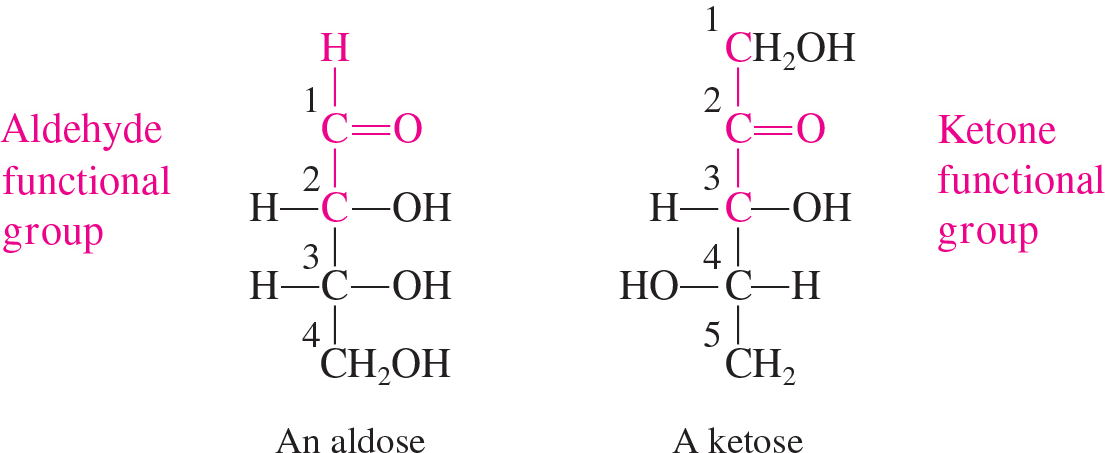
\includegraphics[width=0.7\linewidth]{Aldehyde-Keton}
	\caption[Aldehyden en ketonen]{Aldehyden en ketonen}
	\label{fig:aldehyde-keton}
\end{figure}\\
Naast de aanwezigheid van functionele groepen, maken we ook een onderscheid op basis van het aantal aanwezige koolstof atomen. De nummering en naamgeving van deze moleculen worden overgenomen uit de chemie zoals te zien is op figuur \ref{fig:examples-name}.
\begin{figure}[htbp]
	\centering
	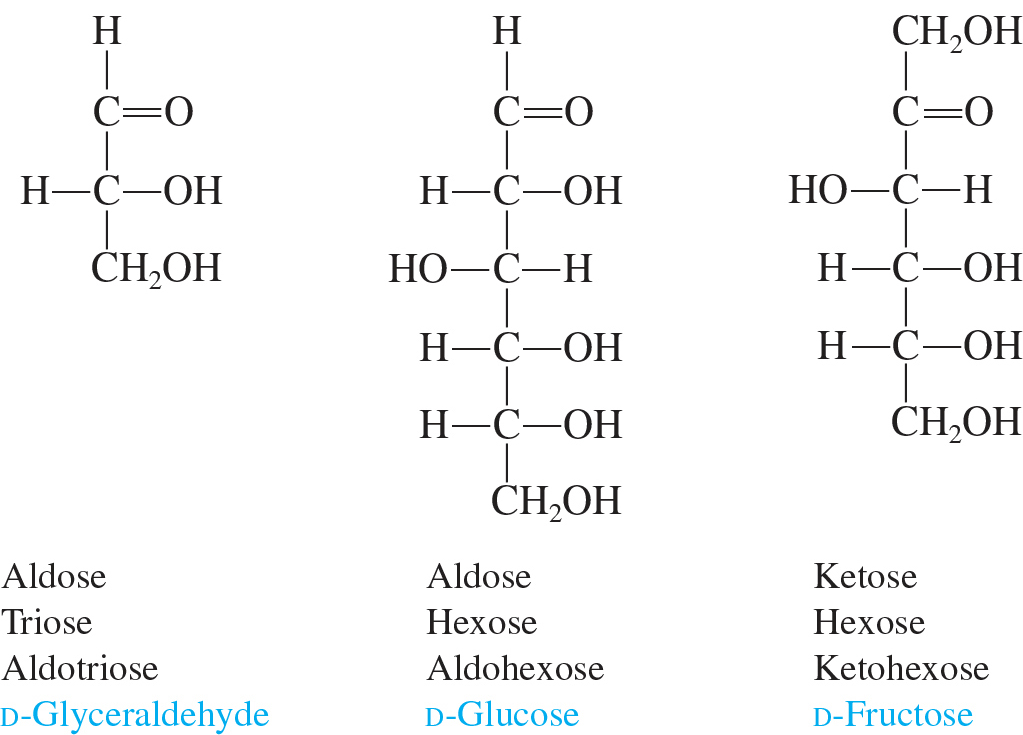
\includegraphics[width=0.6\linewidth]{examples-name}
	\caption[Naamgeving]{Voorbeelden van naamgeving}
	\label{fig:examples-name}
\end{figure}\\
Er zijn ook enkele koolhydraten die een triviale naam krijgen, zoals sacharose of fructose.

\subsection{Voorstellingen}
Er bestaan twee manieren om een koolhydraat voor te stellen, de Fischer- en Haworthprojectie. Voor D-glucose zien we op figuur \ref{fig:fishervshaworth} beide voorstellingen.
\begin{figure}[h]
	\centering
	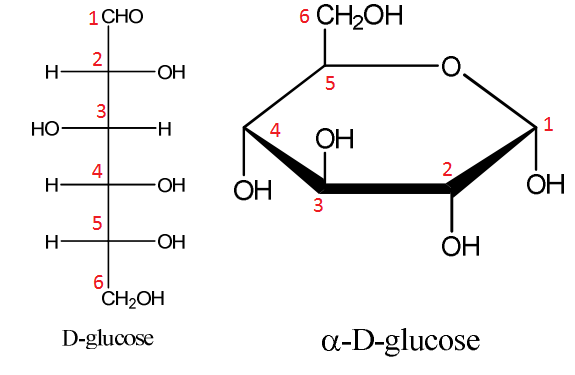
\includegraphics[width=0.6\linewidth]{FisherVSHaworth}
	\caption[Fischer- en Haworthprojectie]{Fischerprojectie (links) en Haworthprojectie (rechts)}
	\label{fig:fishervshaworth}
\end{figure}

\subsection{Stereochemie}
Als de structuur van een koolhydraat koolstof atomen bevat die gebonden zijn met vier verschillende groepen, dan zeggen we dat de structuur een chiraal centrum heeft. Dit fenomeen kan tot opmerkelijke resultaten leiden, zo is het mogelijk dat bepaalde functionele groepen niet altijd op dezelfde manier georiënteerd zijn.  
\subsubsection{Enantiomeren}
\label{sec:enantiomeren}
We spreken van enantiomeren als een we te maken hebben met een molecule die volledig gespiegeld kan worden. Een voorbeeld is te zien op figuur \ref{fig:enantiomeren}. Deze spiegeling heeft enkele gevolgen, zowel op biologisch als op fysisch vlak. Zo kunnen verschillende enantiomeren anders reageren op gepolariseerd licht. Vanuit een biologisch standpunt vormt er een probleem als de enantiomeren niet op dezelfde manier samenwerken met enzymen (zie figuur \ref{fig:enantiomeerenzym}). Als beide enantiomeren (normaal en gespiegeld of L en D in een biologische context) aanwezig zijn in een mengsel, dan nomen we dit een racemisch mengsel.
Het is ook belangrijk om op te merken dat een gespiegelde tekening niet zomaar een enantiomeer is. Het is ook mogelijk dat er een mesoverbinding aan het werk is. Dit is een verbinding met twee of meer chirale koolstofatomen en een intern symmetrievlak zoals te zien is op figuur \ref{fig:mesoverbinding}. 
\begin{figure}
	\centering
	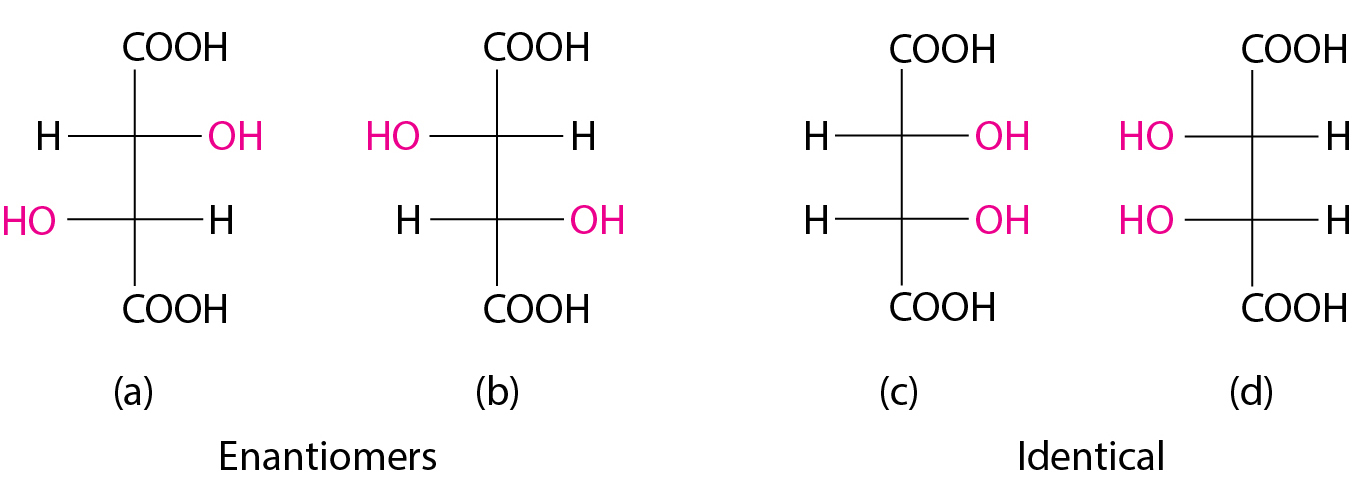
\includegraphics[width=0.7\linewidth]{mesoverbinding}
	\caption[Mesoverbinding]{Enantiomeer (links) en mesoverbinding (rechts)}
	\label{fig:mesoverbinding}
\end{figure}

\begin{figure}[htbp]
	\centering
	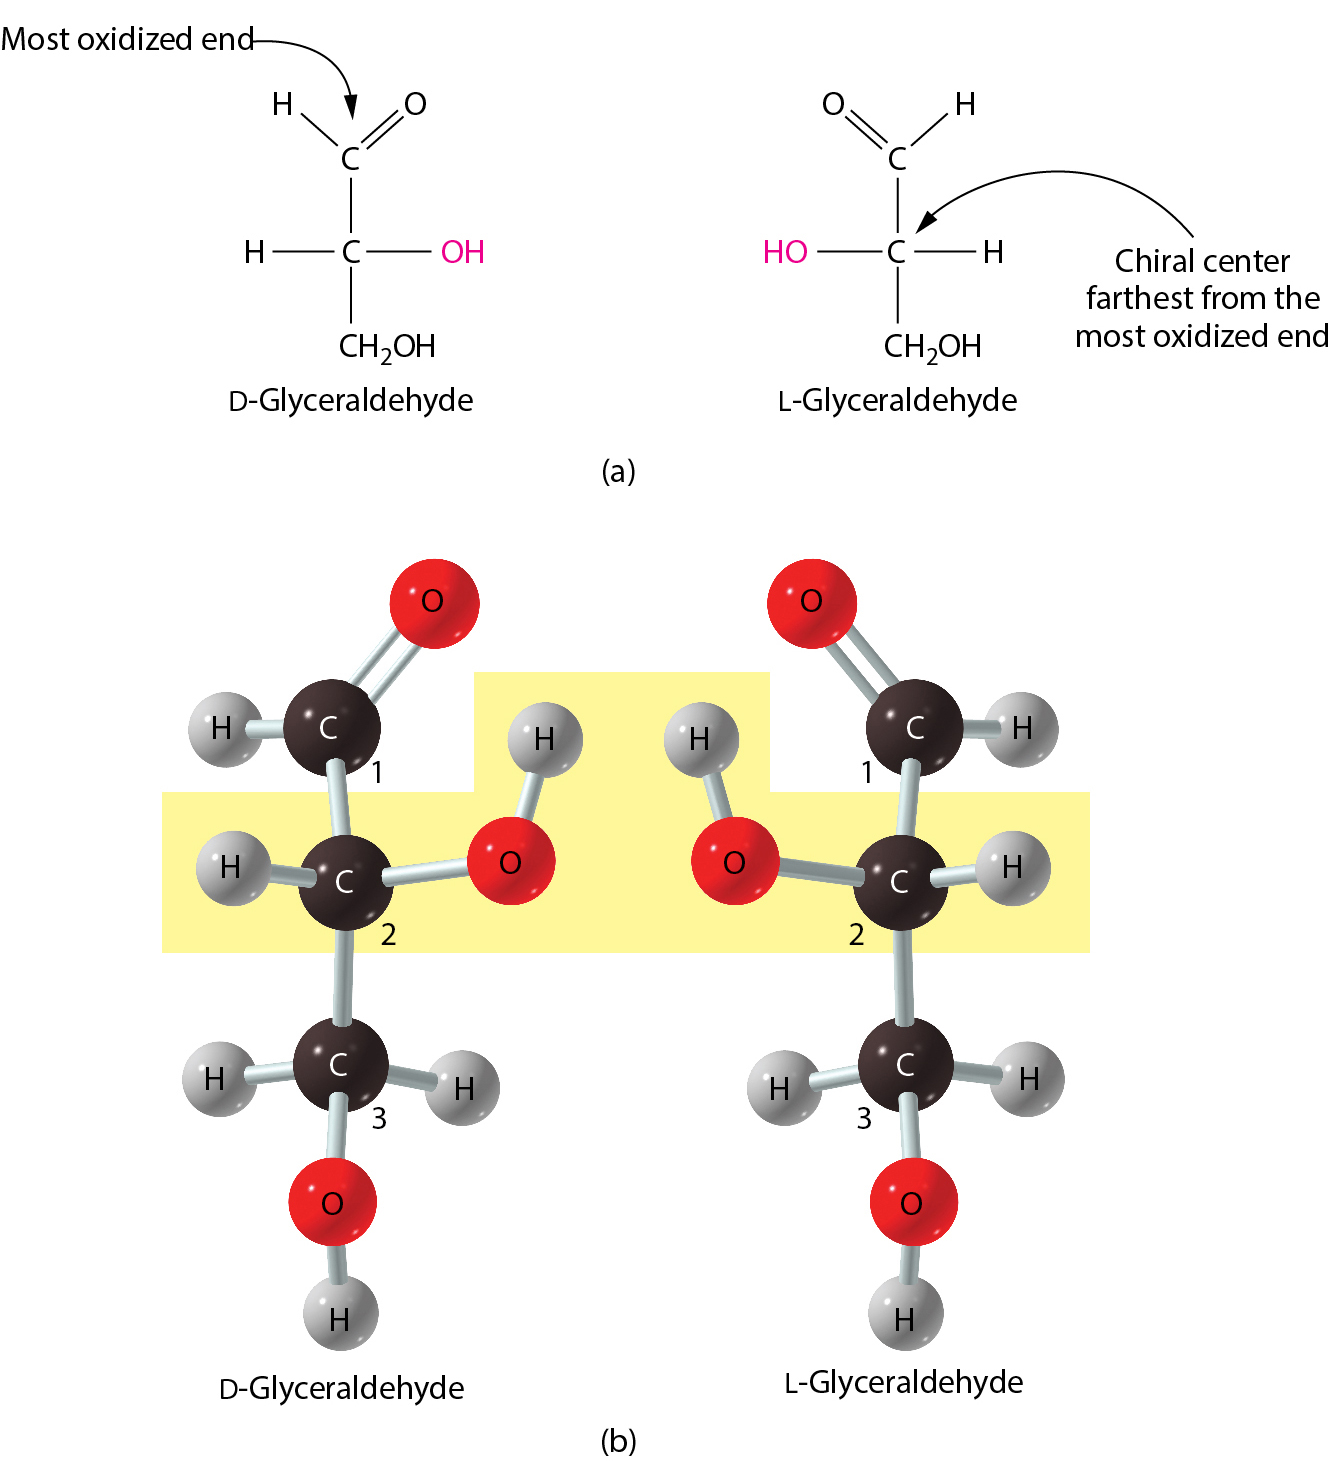
\includegraphics[width=0.6\linewidth]{enantiomeren}
	\caption[Enantiomeer]{Enantiomeer}
	\label{fig:enantiomeren}
\end{figure}
\begin{figure}[htbp]
	\centering
	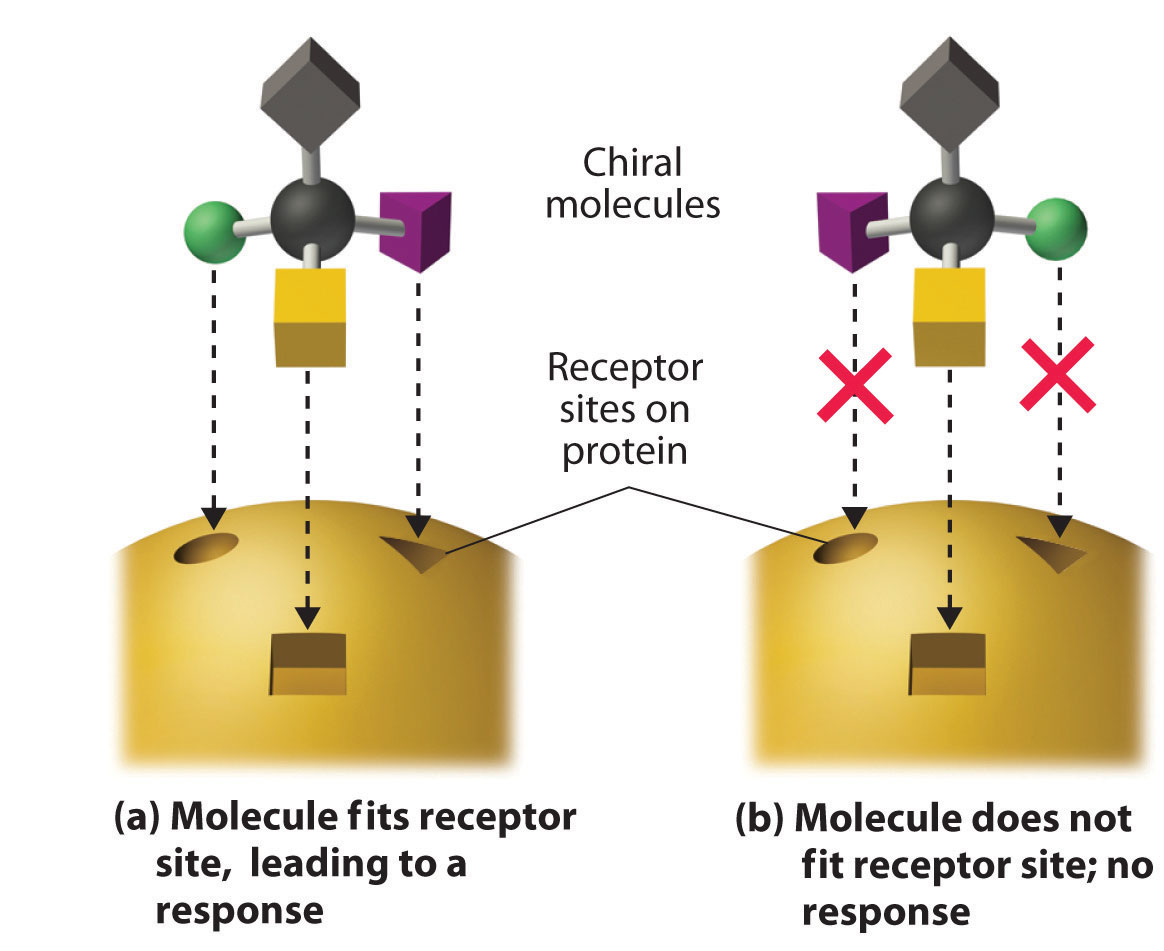
\includegraphics[width=0.5\linewidth]{EnantiomeerEnzym}
	\caption[Enantiomeer en enzym]{Interactie tussen enantiomeren en enzymen}
	\label{fig:enantiomeerenzym}
\end{figure}


\subsubsection{Diastereomeren}
\begin{figure}[htbp]
	\centering
	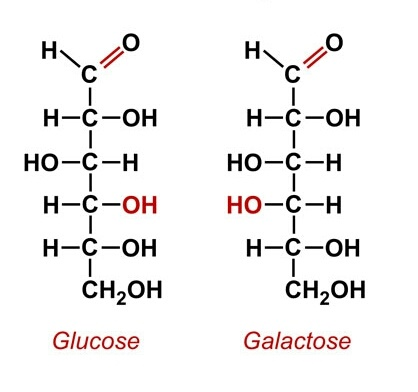
\includegraphics[width=0.4\linewidth]{Diastereomeren}
	\caption[Diastereomeren]{Diastereomeren}
	\label{fig:diastereomeren}
\end{figure}
Diastereomeren zijn zoals enantiomeren, maar ze zijn geen perfect spiegelbeeld zoals te zien is op figuur \ref{fig:diastereomeren}.
\subsubsection{Glucose}
Het bekendste voorbeeld van dit fenomeen is glucose. In de natuur observeren we D-glucose en L-glucose. Hiervan zien we voornamelijk D-glucose voorkomen omdat dit het type glucose is dat gemaakt wordt door fotosynthese. Ons lichaam maakt wel een onderscheid tussen beide varianten, ze smaken alle twee zoet maar enkel D-glucose heeft een calorische inhoud bij het verteren. Dit wil zeggen dat L-glucose niet wordt opgenomen door ons spijsverterings-stelsel, en dus niet kan  gebruikt worden om energie uit te halen. Het is dus een `zoetstof'.

\subsection{Reducerende koolhydraten}
We spreken van een reducerend koolhydraat als het molecuul optreedt als reducerend agens in een redox-reactie als gevolg van de aanwezigheid van de aldehyde- of ketongroep (zie figuur \ref{fig:reductiefding}). Veel monosachariden bezitten deze eigenschap, daarnaast hebben ook disachariden, waarvan het anomere koolstof-atoom geen glycoside binding heeft, ook een reducerend vermogen. Polysachariden hebben meestal een te lage hoeveelheid reducerende uiteinden om een reductief karakter te hebben.
\begin{figure}[htbp]
	\centering
	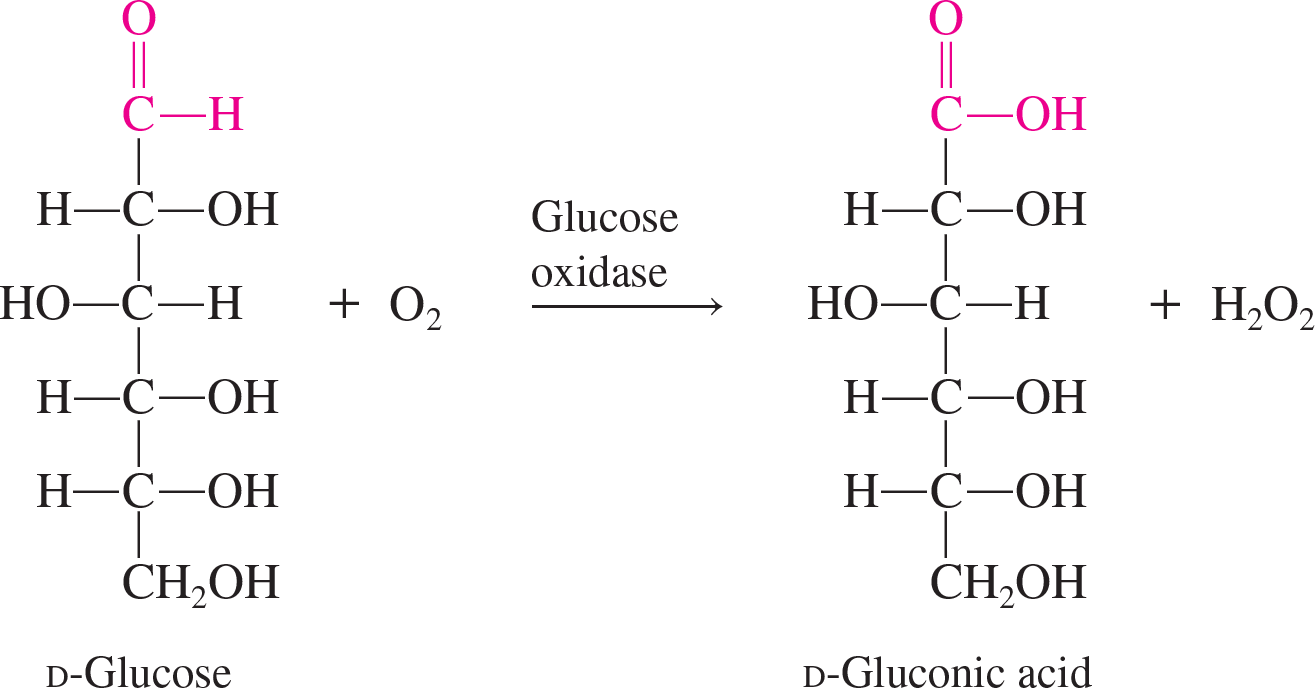
\includegraphics[width=0.5\linewidth]{ReductiefDing}
	\caption[Reducerende koolhydraten]{Reducerende koolhydraten}
	\label{fig:reductiefding}
\end{figure}\\
We kunnen testen of een koolhydraat in het bezit is van een reducerend karakter met Benetict's reagens. Hierbij kijken we naar de kleurverandering van de oplossing na de reactie. Dit is tevens de manier waarop we kunnen bepalen of er suiker in urine zit, het is handig om suikerziekte op te sporen.

\subsection{Monosachariden}
Monosachariden zijn de meest eenvoudige koolhydraten. Ze vormen hierdoor dus ook de bouwstenen voor complexere structuren zoals disachariden en polysachariden. 
\subsubsection{Belangrijke monosachariden}
In monosachariden merken we telkens anomeren op. Een anomeer is een stereo-isomeer van een koolhydraat in ringvorm met het enigste verschil de configuratie van het koolstof-atoom op positie 1. \\
\textbf{Glucose}
\begin{figure}[h]
	\centering
	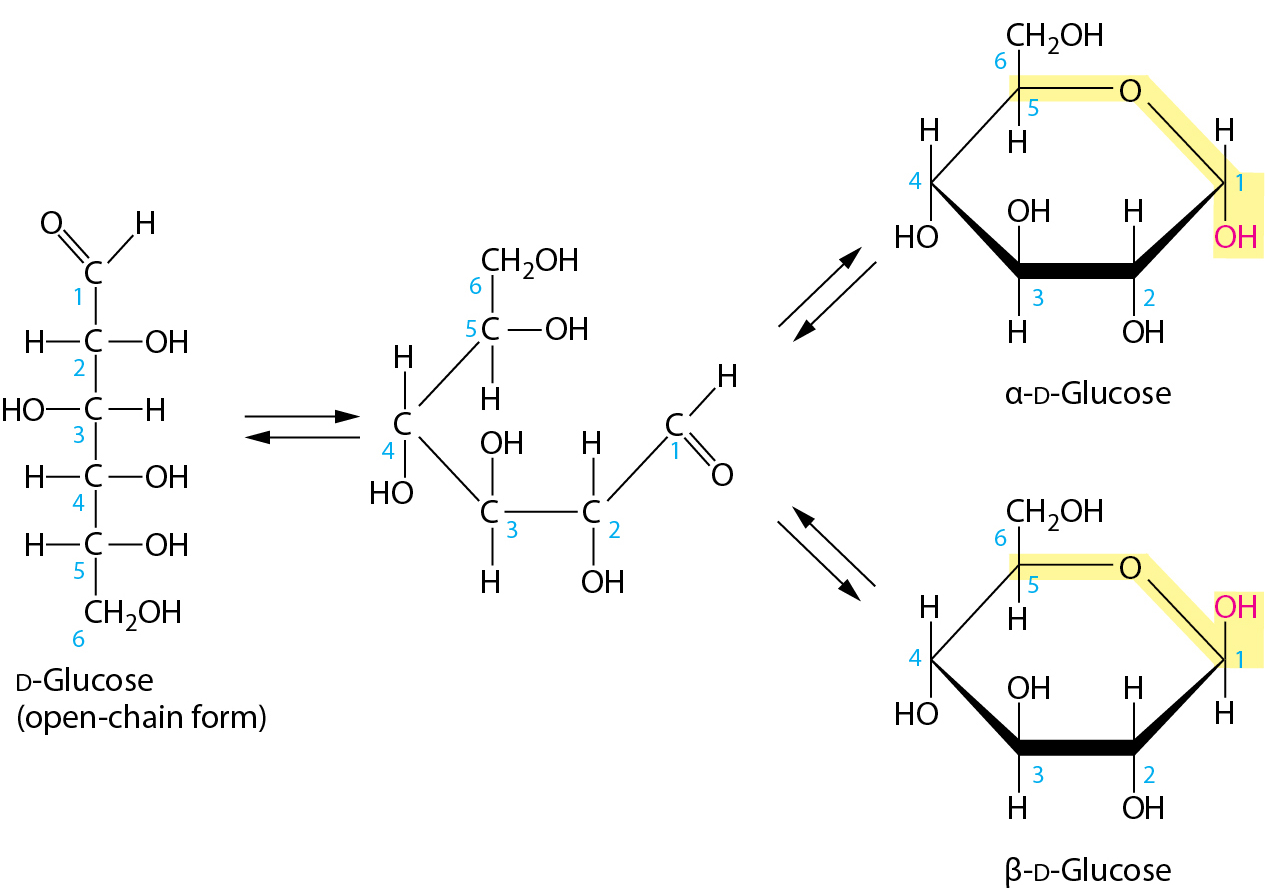
\includegraphics[width=0.7\linewidth]{GlucoseAlphaBeta}
	\caption[Glucose]{Glucose}
	\label{fig:glucosealphabeta}
\end{figure}\\
Hierbij kunnen we nog vermelden dat koolstof atoom 1 in figuur \ref{fig:glucosealphabeta} een nieuw chiraal centrum is, en dus een anomeer C-atoom is.\\
\textbf{Fructose}
\begin{figure}[h]
	\centering
	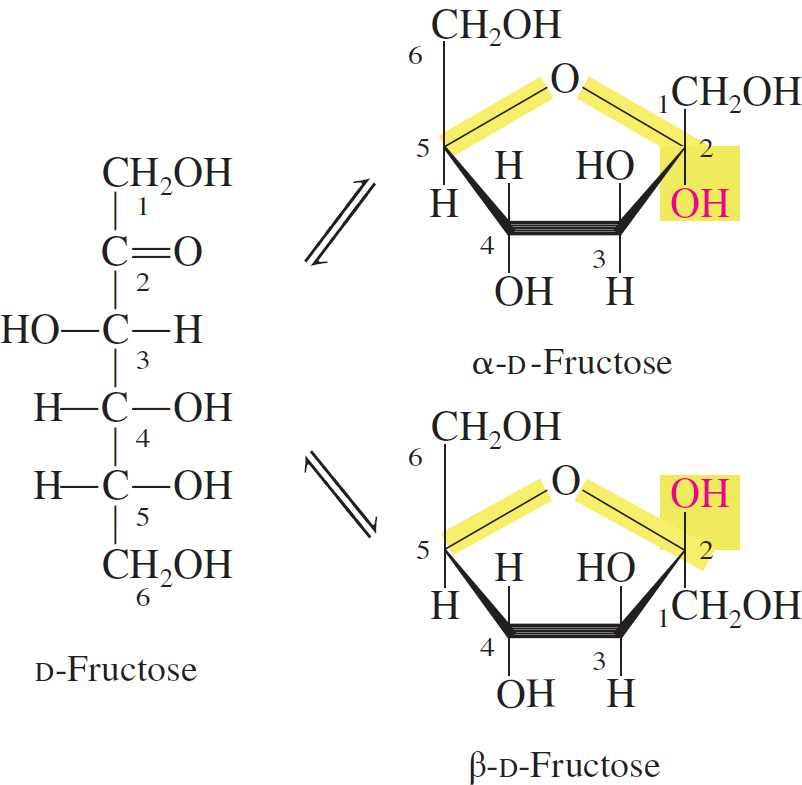
\includegraphics[width=0.4\linewidth]{FructoseAlphaBeta}
	\caption[Fructose]{Fructose}
	\label{fig:fructosealphabeta}
\end{figure}\\
Hierbij kunnen we nog vermelden dat koolstof atoom 2 in figuur \ref{fig:fructosealphabeta} een nieuw chiraal centrum is, en dus een anomeer C-atoom is.\\
\newpage
\textbf{Deoxyribose}
\begin{figure}[h]
	\centering
	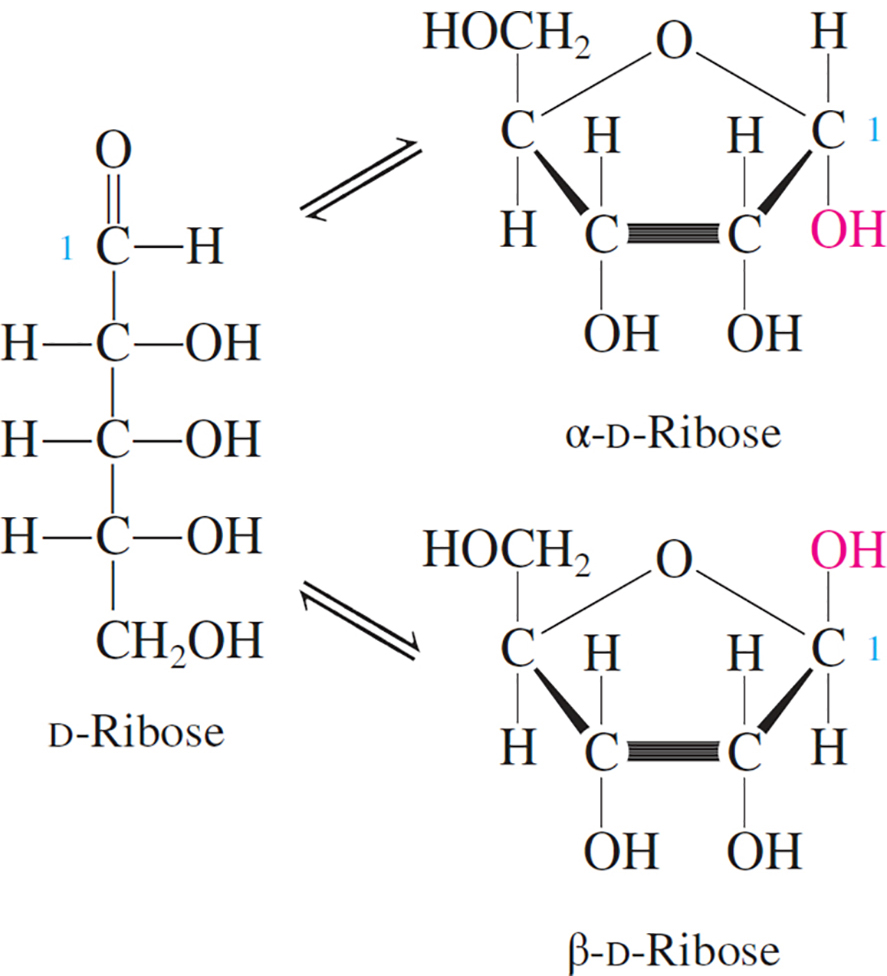
\includegraphics[width=0.4\linewidth]{deoxyribosealphabeta}
	\caption[Deoxyribose]{Deoxyribose}
	\label{fig:deoxyribosealphabeta}
\end{figure}\\
Hierbij kunnen we nog vermelden dat koolstof atoom 1 in figuur \ref{fig:deoxyribosealphabeta} een nieuw chiraal centrum is, en dus een anomeer C-atoom is. Deoxyribose is tevens belangrijk voor RNA en DNA.\\
\textbf{Acetylglucosamine}\\
Door andere functionele groepen toe te voegen aan de koolhydraatstructuur kunnen we complexere moleculen maken. Acetylglucosamine (figuur \ref{fig:acetylglucosamine}) is bijvoorbeeld een bloed antigen.
\begin{figure}[h]
	\centering
	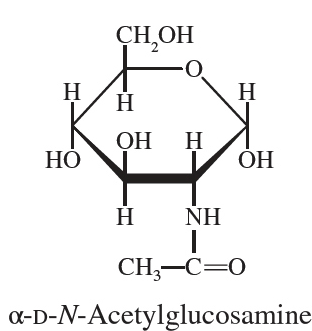
\includegraphics[width=0.4\linewidth]{Acetylglucosamine}
	\caption[Acetylglucosamine]{Acetylglucosamine}
	\label{fig:acetylglucosamine}
\end{figure}
\subsubsection{Afgeleiden}
Enkele voorbeelden van afgeleiden van monosachariden zijn polyolen. Ze zijn geen monosachariden, maar lijken er wel sterk op. De voorbeelden uit figuur \ref{fig:afgeleidenmonosachariden} zijn zoet zoals glucose, ze hebben wel geen calorie-inhoud. Ze zijn dus geschikt om zoetstoffen mee te maken.
\begin{figure}[h]
	\centering
	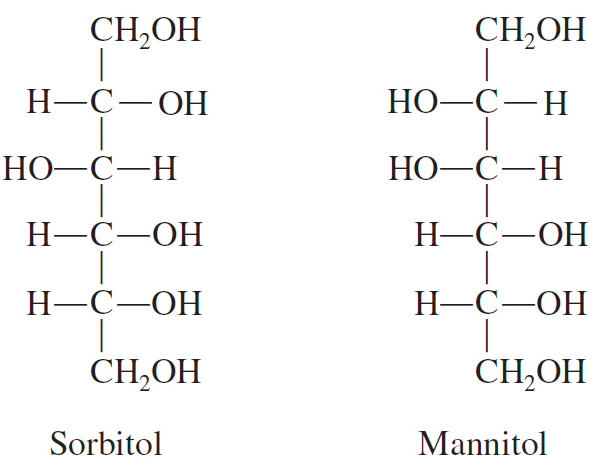
\includegraphics[width=0.4\linewidth]{AfgeleidenMonosachariden}
	\caption[Afgeleiden]{Afgeleiden van monosachariden}
	\label{fig:afgeleidenmonosachariden}
\end{figure}

\subsection{Disachariden}
Disachariden zijn opgebouwd uit 2 monosachariden. We kunnen ze benoemen volgens de monosachariden waaruit ze zijn opgebouwd, en de manier waarop deze gebonden zijn aan elkaar.
\subsubsection{Belangrijke disachariden}
\textbf{Sucrose}\\
Sucrose is wat wij kennen als 'gewoon' suiker. Het is opgebouwd uit $\alpha$-glucose en $\beta$-Fructose (zie figuur \ref{fig:sucrose}).
\begin{figure}[h]
	\centering
	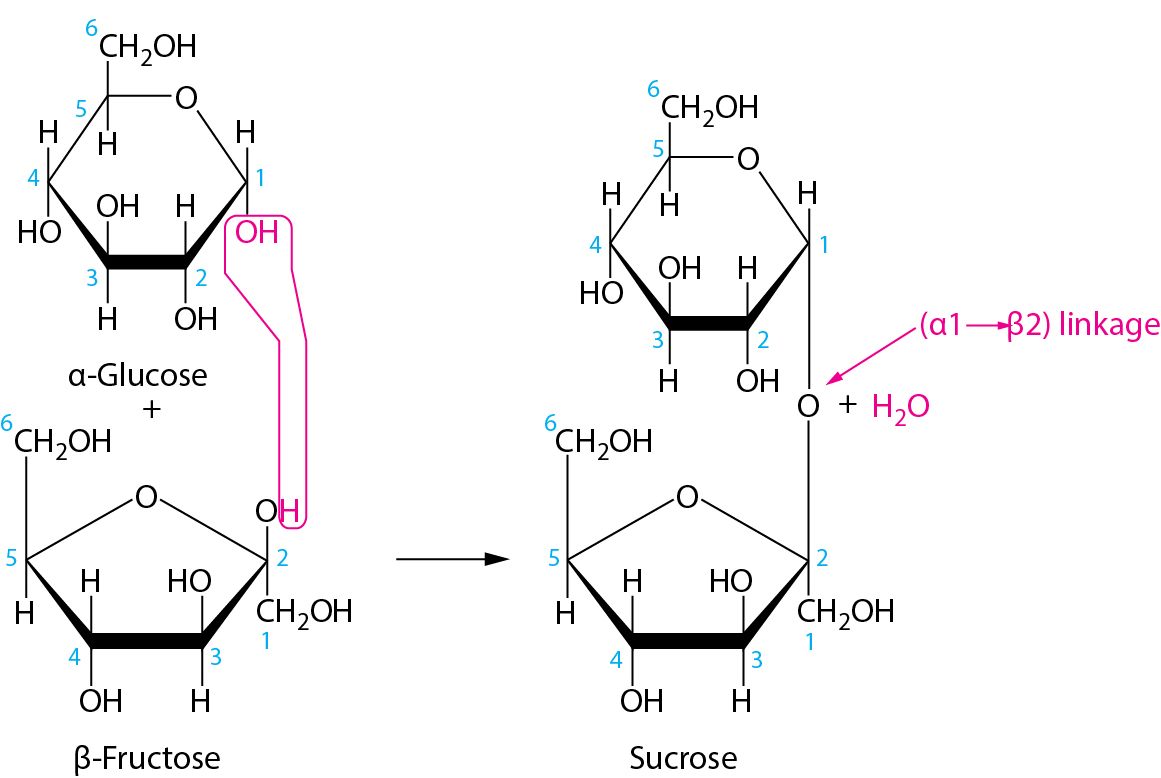
\includegraphics[width=0.5\linewidth]{sucrose}
	\caption[Sucrose]{Sucrose}
	\label{fig:sucrose}
\end{figure}\\
\textbf{Lactose}\\
Lactose of melksuiker is opgebouwd uit $\beta$-D-galactose en $\beta$-D-glucose (zie figuur \ref{fig:lactose}).
\begin{figure}[h]
	\centering
	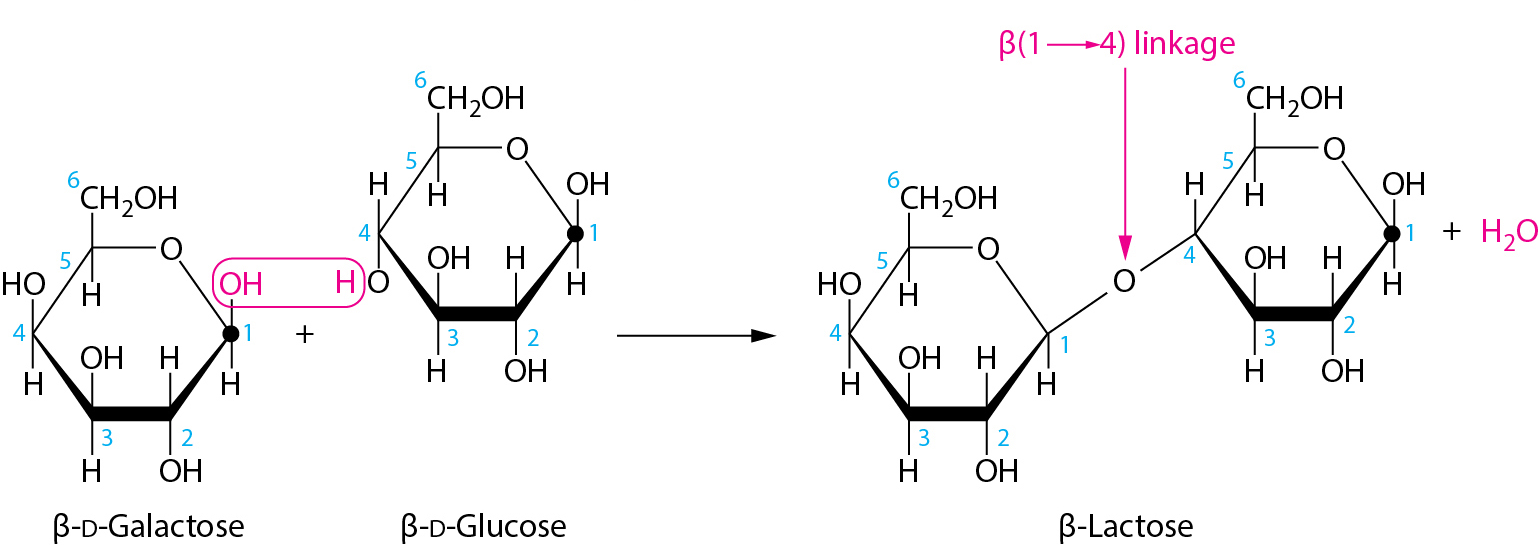
\includegraphics[width=0.6\linewidth]{Lactose}
	\caption[Lactose]{Lactose}
	\label{fig:lactose}
\end{figure}\\ 
\newpage 	
\textbf{Maltose}\\
Maltose of moutsuiker is opgebouwd uit $\alpha$-D-glucose en $\beta$-D-glucose (zie figuur \ref{fig:maltose}).
\begin{figure}[h]
	\centering
	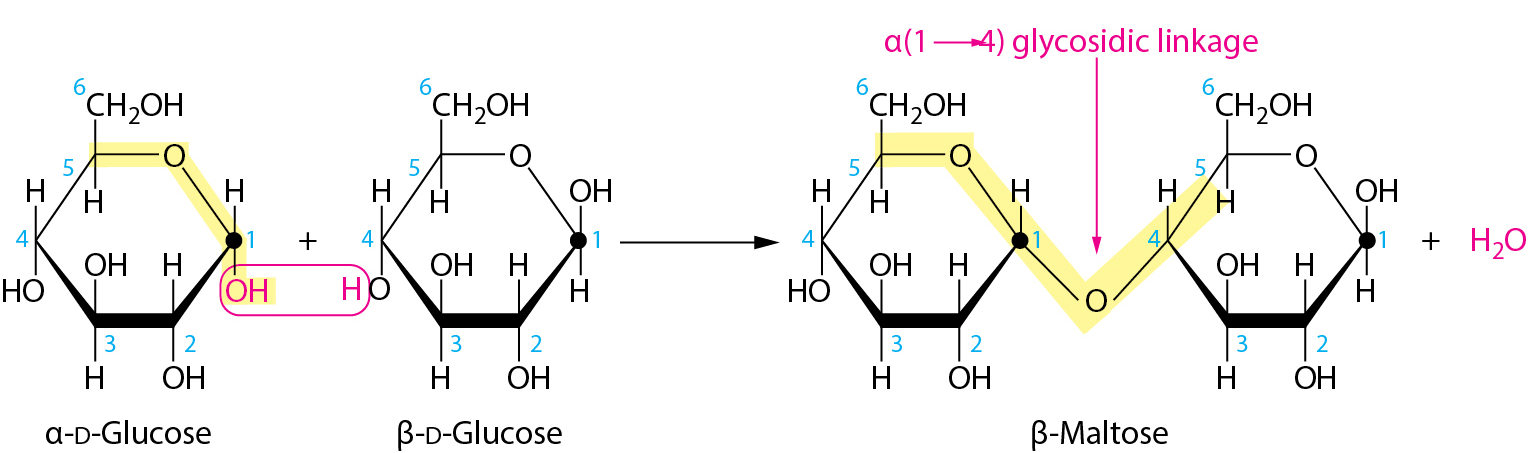
\includegraphics[width=0.6\linewidth]{Maltose}
	\caption[Maltose]{Maltose}
	\label{fig:maltose}
\end{figure}

\subsection{Polysachariden}
Polysachariden zijn net zoals disachariden opgebouwd uit monosachariden. Het verschil zit in de hoeveelheid bouwblokken er aanwezig zijn. Grosso modo zullen we spreken over polysachariden als er meer dan 2 monosachariden betrokken zijn bij de opbouw.

Afhankelijk van de onderlinge bindingen, kunnen er zich vertakkingen voor doen in een polysacharide. beide polysachariden in figuur \ref{fig:vertakkingen} zijn opgebouwd volgens de structuur in figuur \ref{fig:vertakking}. Door het aanzienlijke verschil in vertakkingen, maken we een onderscheid tussen deze twee moleculen.
\begin{figure}[h]
	\centering
	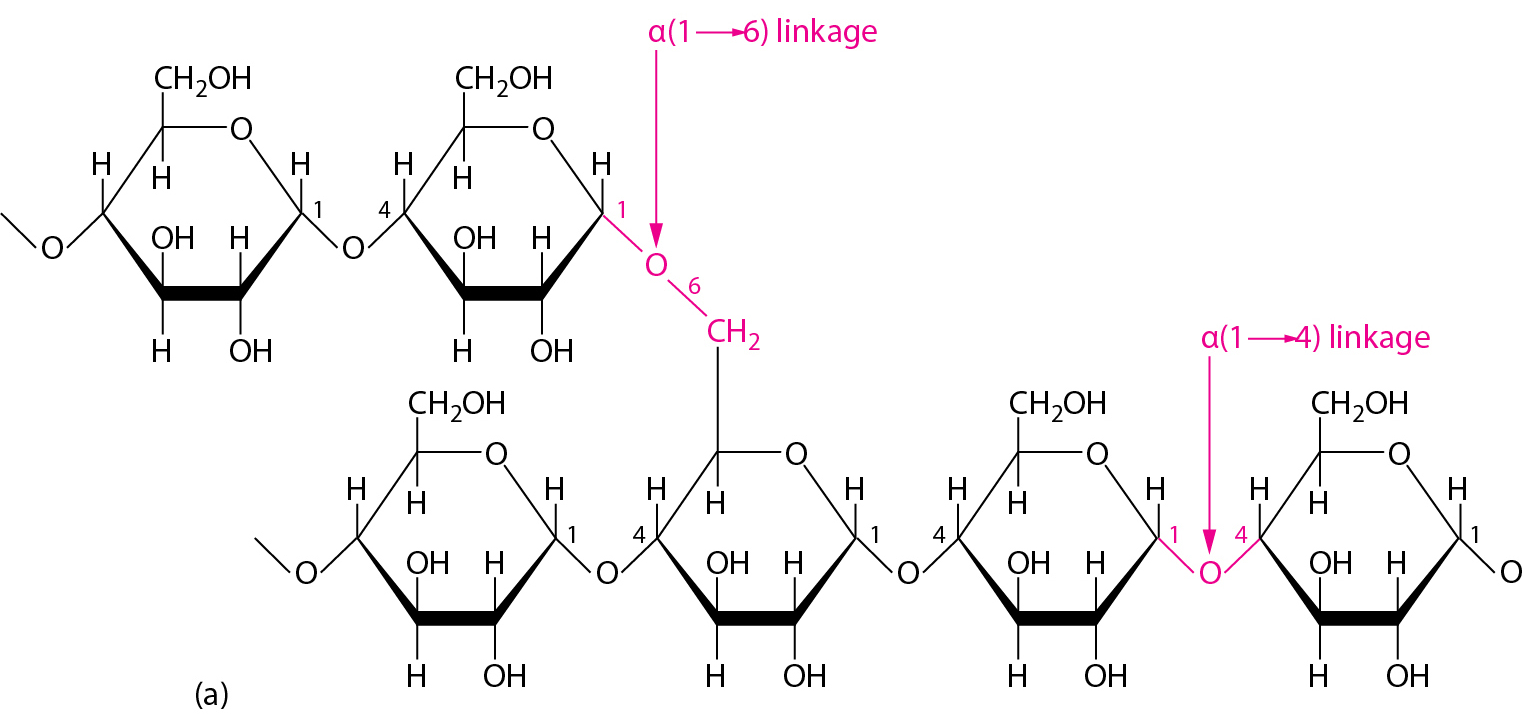
\includegraphics[width=0.7\linewidth]{Vertakking}
	\caption[Vertakking]{Verschillende bindingen zorgen voor vertakkingen}
	\label{fig:vertakking}
\end{figure}

\begin{figure}[h]
	\centering
	\begin{subfigure}{.5\textwidth}
		\centering
		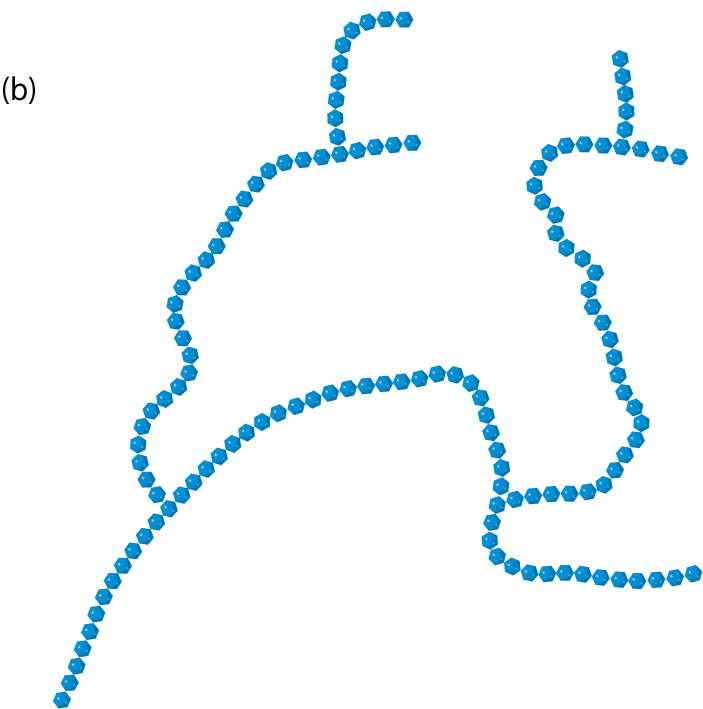
\includegraphics[width=.4\linewidth]{amylopectine_in_zetmeel.png}
		\caption{Amylopectine in zetmeel}
		\label{fig:sub1}
	\end{subfigure}%
	\begin{subfigure}{.5\textwidth}
		\centering
		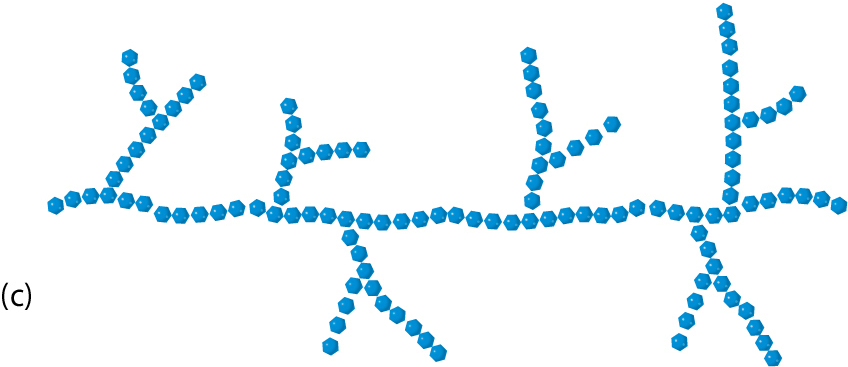
\includegraphics[width=.7\linewidth]{Glycogeen.png}
		\caption{Glycogeen}
		\label{fig:sub2}
	\end{subfigure}
	\caption{Het verschil tussen veel en weinig vertakkingen}
	\label{fig:vertakkingen}
\end{figure}
\newpage
\subsubsection{Belangrijke polysachariden}
\textbf{Zetmeel en glycogeen}\\
Zetmeel en glycogeen lijken sterk op elkaar, ze zijn beiden namelijk opgebouwd volgens figuur \ref{fig:vertakking}. Zetmeel vinden we voornamelijk terug in planten, het is een belangrijke nutriënt voor de mens. We gebruiken het namelijk vaak voor het maken van brood en pasta. Een bijkomend voordeel, is dat het gemakkelijk afbreekbaar is tijdens de vertering. Glycogeen komt hoofdzakelijk voor bij dieren. Het is in grote concentraties aanwezig in spierweefsel en de lever. Dit is ook de meer vertakte variant van amylopectine (zie figuur \ref{fig:vertakkingen}).\\
\textbf{Cellulose}\\
Cellulose is vaak aanwezig bij planten. Het is niet verteerbaar door de mens, dit wil zeggen dat er eigenlijk geen calorische inhoud is. Het kan vaak gebruikt worden als een structureel component om een cel op te bouwen omdat het een soort vezel vormt. Dit is ook de reden waarom we cellulose gebruiken om papier te maken. De structuur van cellulose is te zien in figuur \ref{fig:cellulose}.
\begin{figure}[h]
	\centering
	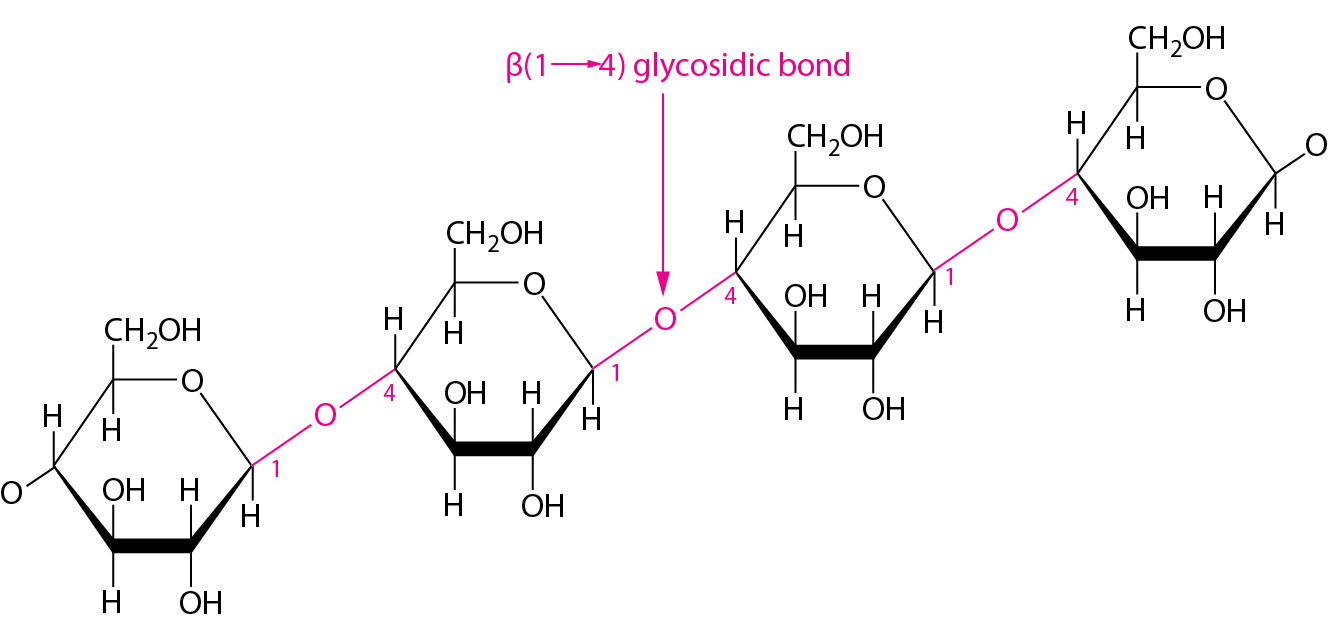
\includegraphics[width=0.7\linewidth]{Cellulose}
	\caption[Cellulose]{Cellulose}
	\label{fig:cellulose}
\end{figure}

\section{Lipiden}
\begin{figure}[htbp]
	\centering
	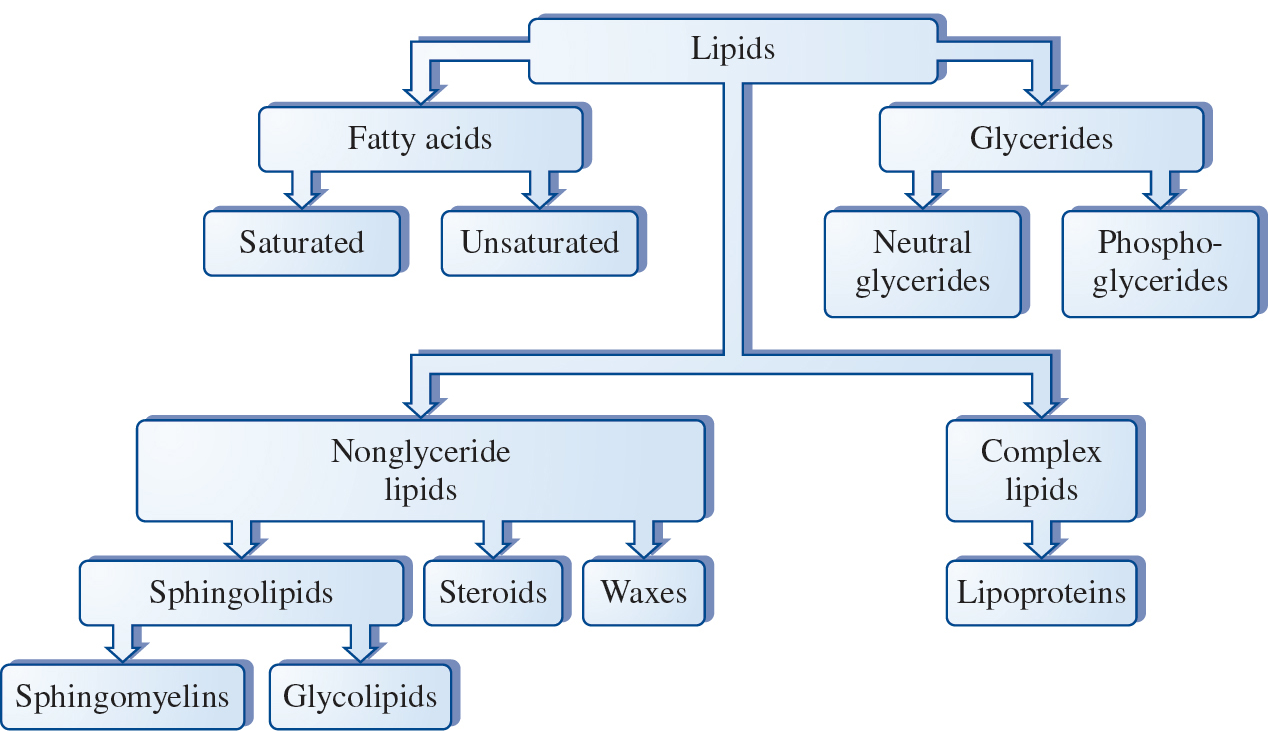
\includegraphics[width=0.7\linewidth]{Schema_lipiden}
	\caption[Lipiden]{Schema van lipiden}
	\label{fig:schemalipiden}
\end{figure}

%Overzicht Schema slide 28
\subsection{Biologische functies van lipiden}
Biologisch gezien zijn vetten extreem belangrijk. De mens gebruikt ze namelijk voor verschillende doeleinden:
\begin{itemize}
	\item Energiebron en -opslag
	\item Structurele componenten van het celmembraan
	\item Hormonen
	\item Vitaminen en vitamine-adsorptie
	\item Bescherming
	\item Isolatie
\end{itemize}
\subsection{Vetzuren}
\subsubsection{Structuur}
Vetzuren hebben lange ketens van monocarboxylzuren (-COOH) met een even aantal koolstofatomen (zie figuur \ref{fig:structuurvetzuur}).
\begin{figure}[h]
	\centering
	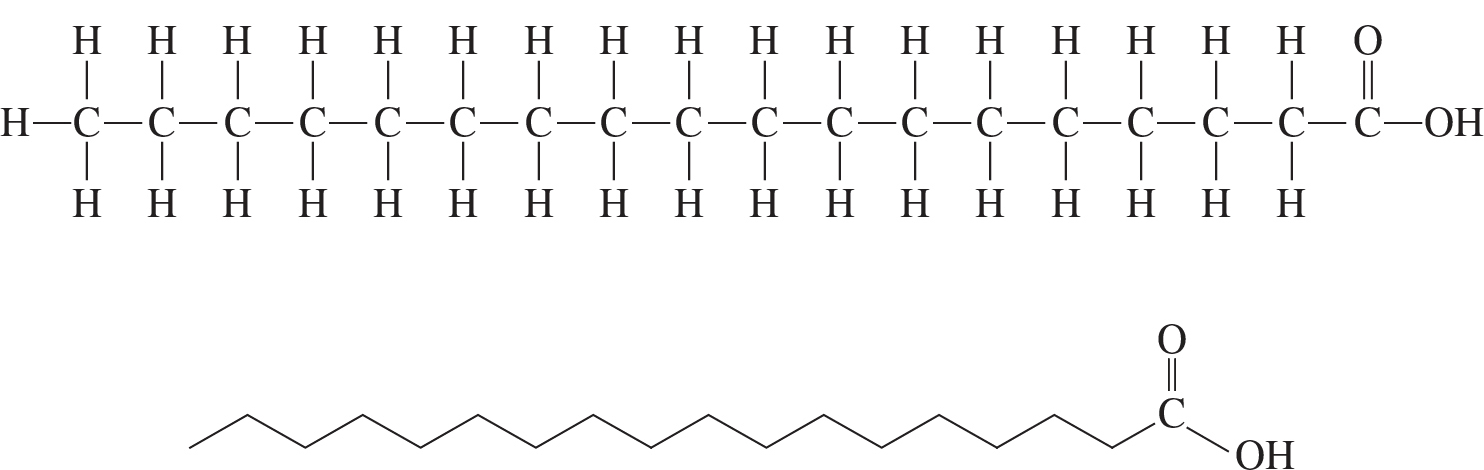
\includegraphics[width=0.7\linewidth]{StructuurVetZuur}
	\caption[Vetzuur]{Structuur van een vetzuur}
	\label{fig:structuurvetzuur}
\end{figure}
\subsubsection{(On)Verzadigde vetzuren}
Verzadigde vetzuren bestaan uitsluitend uit enkelvoudig gebonden koolstof atomen zoals in figuur \ref{fig:structuurvetzuur}. We spreken van een onverzadigd vetzuur als er een dubbele binding voorkomt tussen de koolstoffen zoals in figuur \ref{fig:onverzadigdevetzuren}.
\begin{figure}[h]
	\centering
	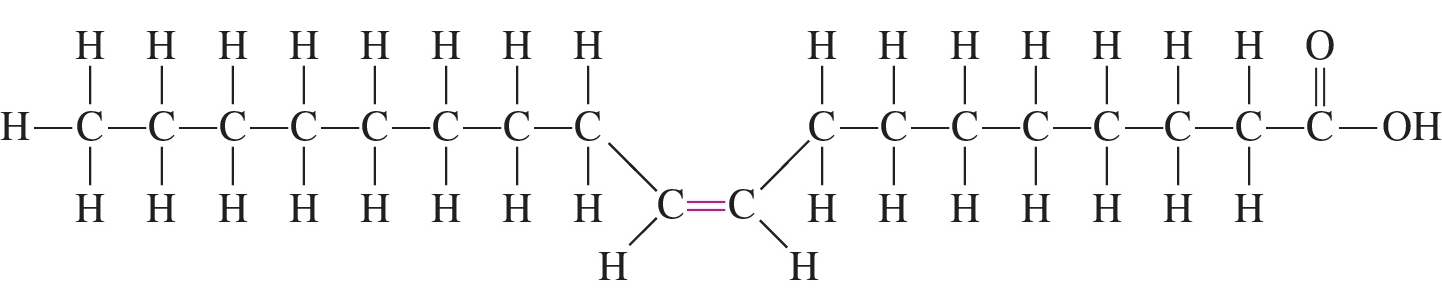
\includegraphics[width=0.7\linewidth]{OnVerzadigdeVetzuren}
	\caption[Onverzadigde VZ]{Onverzadigde vetzuren}
	\label{fig:onverzadigdevetzuren}
\end{figure}\\
We vinden verzadigde vetzuren vaak bij dieren en onverzadigde vetzuren bij planten. Ook het smeltpunt kent grote verschillen tussen beide soorten (zie figuur \ref{fig:smeltpuntvetzuren}). Grosso modo kunnen we zeggen dat het smeltpunt van verzadigde vetzuren afhangt van de lengte van de koolstofketen (London krachten). Bij onverzadigde vetzuren is het smeltpunt invers proportioneel aan het aantal onverzadigde bindingen. 
\begin{figure}[h]
	\centering
	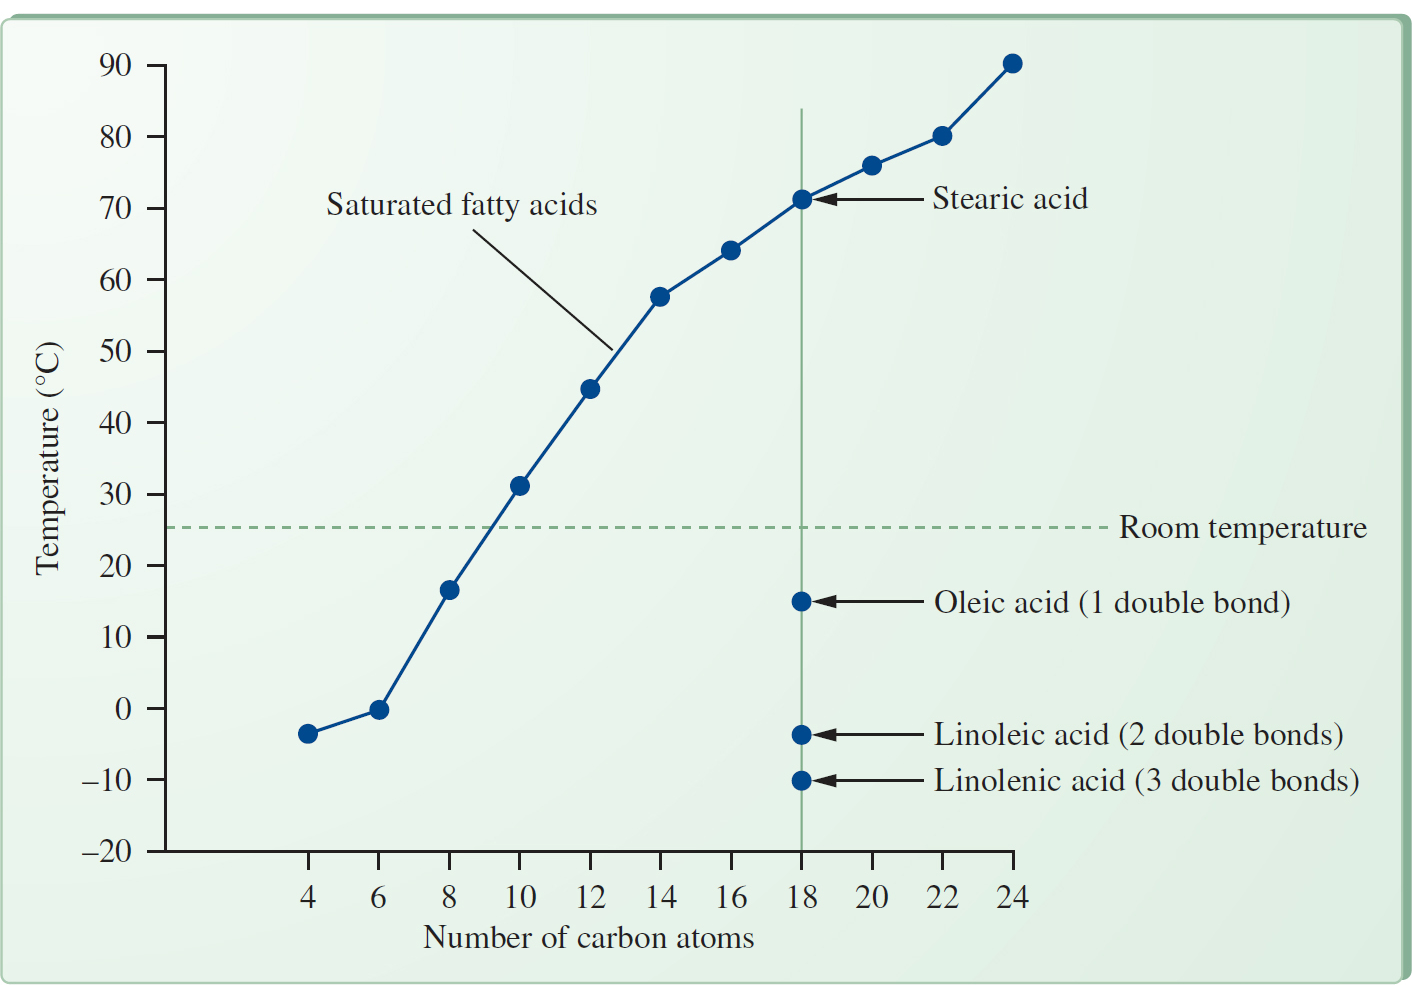
\includegraphics[width=0.7\linewidth]{smeltpuntVetzuren}
	\caption[Smeltpunt]{Smeltpunt van verzadigde en onverzadigde vetzuren}
	\label{fig:smeltpuntvetzuren}
\end{figure}
\subsubsection{Cis- en Transvetzuren}
Het verschil tussen cis- en transvetzuren zit in de manier waarop de koolstof atomen onderling georiënteerd zijn (zie figuur \ref{fig:cistransvz}). Over het algemeen kunnen we zeggen dat transvetzuren slecht zijn voor de mens, ze hebben een negatief effect op zaken zoals cholesterol en hart- en vaatziekten. We vinden ze vaak bij producten gemaakt van herkauwers, en na verhitting van vetzuren. Cisvetzuren daarentegen hebben een positieve invloed op cholesterol.
\begin{figure}[h]
	\centering
	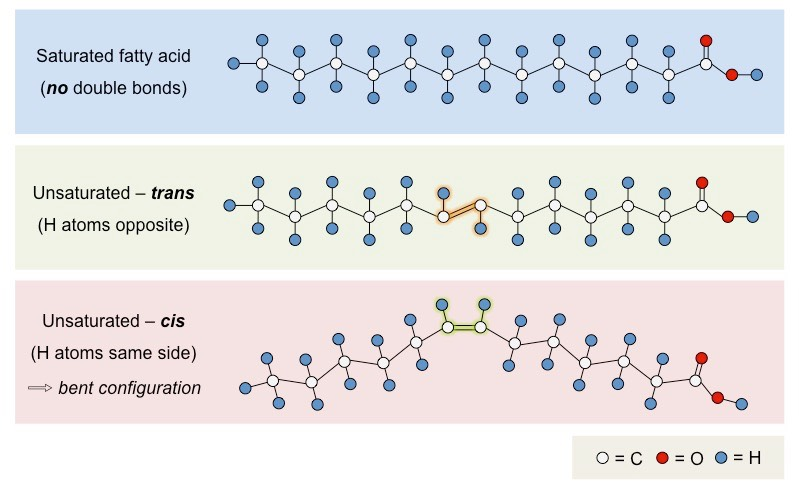
\includegraphics[width=0.7\linewidth]{CisTransVZ}
	\caption[Cis en Trans]{Cis- en Transvetzuren}
	\label{fig:cistransvz}
\end{figure}
\newpage
\subsubsection{Omega vetzuren}
We spreken hoofdzakelijk over omega 3 en omega 6 vetzuren. Het zijn onverzadigde vetzuren die hun naam krijgen op basis van het aantal verzadigde bindingen voor de eerste dubbele binding, zie figuur \ref{fig:omegaVZ}. 
\begin{figure}[h]
	\centering
	\begin{subfigure}{.5\textwidth}
		\centering
		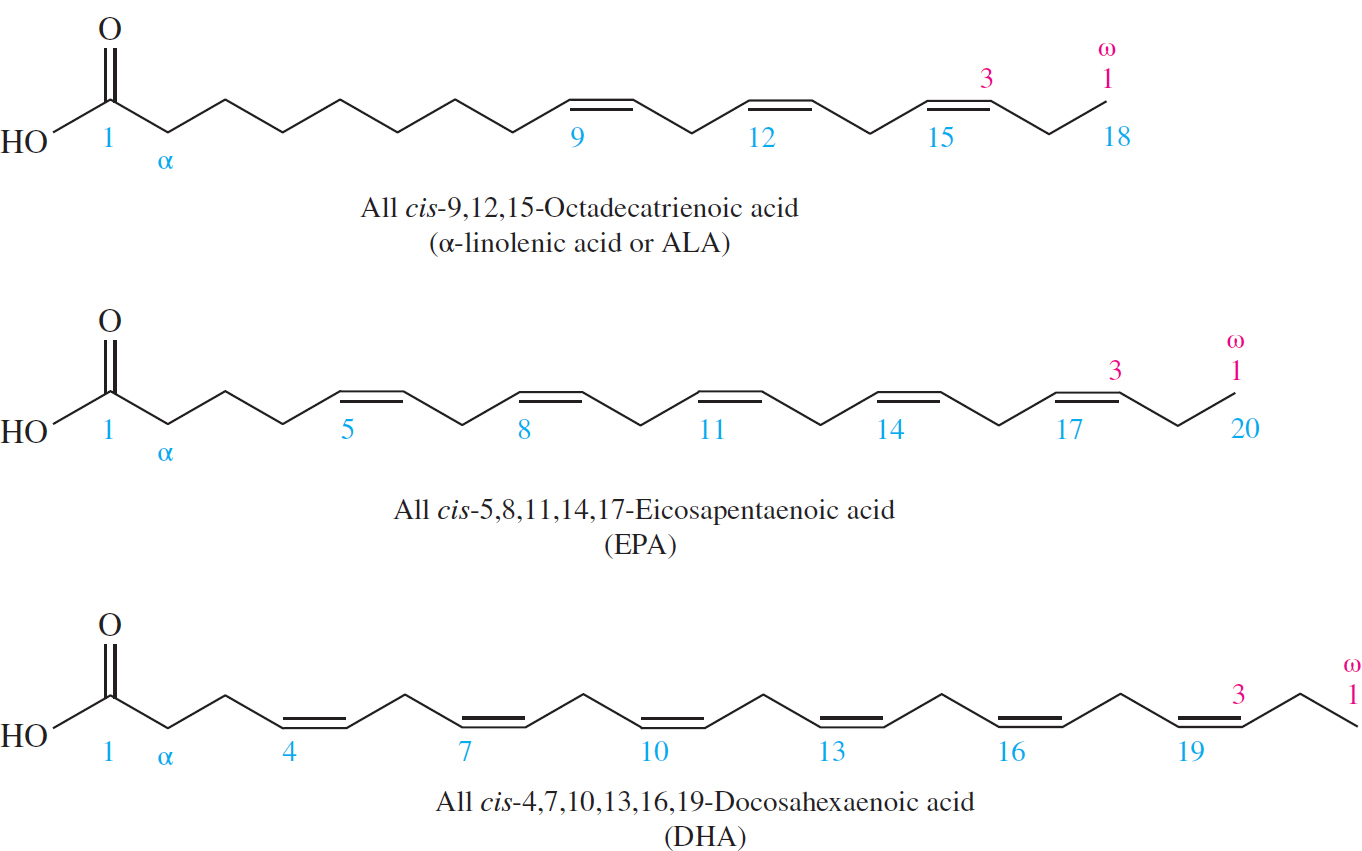
\includegraphics[width=1\linewidth]{Omega3VZ}
		\caption{Omega 3 vetzuur}
		\label{fig:Omega3}
	\end{subfigure}%
	\begin{subfigure}{.5\textwidth}
		\centering
		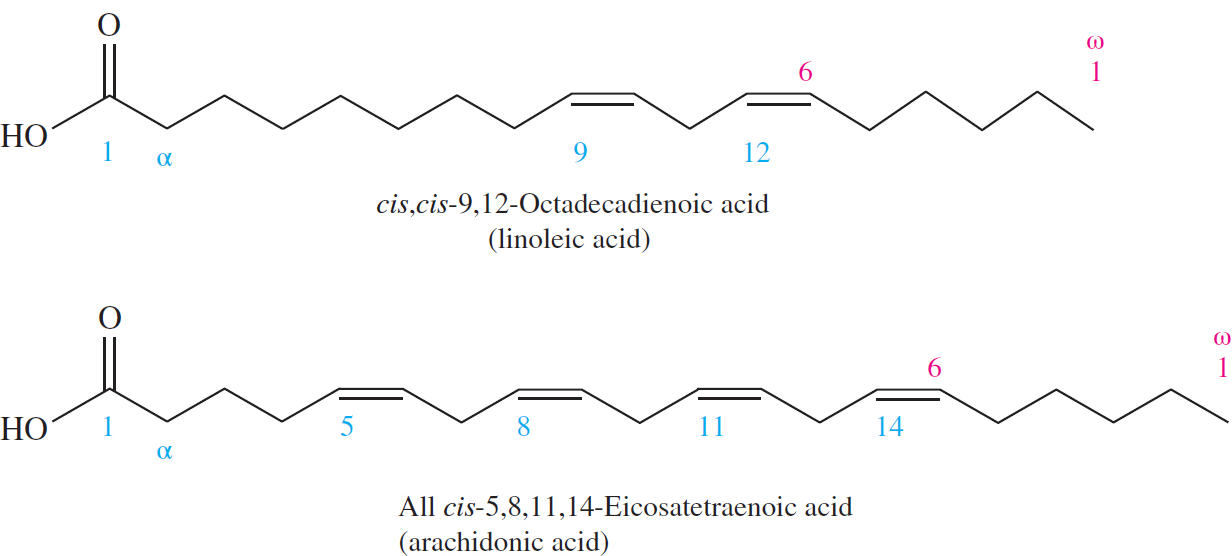
\includegraphics[width=1\linewidth]{Omega6VZ}
		\caption{Omega 6 vetzuur}
		\label{fig:Omega6}
	\end{subfigure}
	\caption{Het verschil tussen veel en weinig vertakkingen}
	\label{fig:omegaVZ}
\end{figure}\\
We associëren omega 3 vetzuren vaak met positieve gezondheidseffecten, onderzoek wijst namelijk uit dat het hart- en vaatziekten tegenhoud en een ontstekingsremmend effect heeft. Omega 6 vetzuren komen met ongewenste gezondheidseffecten.
\subsubsection{Reacties met vetzuren}
De belangrijkste reactie van deze cursus is de hydrogenering (zie figuur \ref{fig:hydrogenering}). Het is een additie reactie waarbij onverzadigde vetzuren omgezet worden in verzadigde vetzuren. Deze reactie wordt sterk gebruikt in de voedingsindustrie.
\begin{figure}[h]
	\centering
	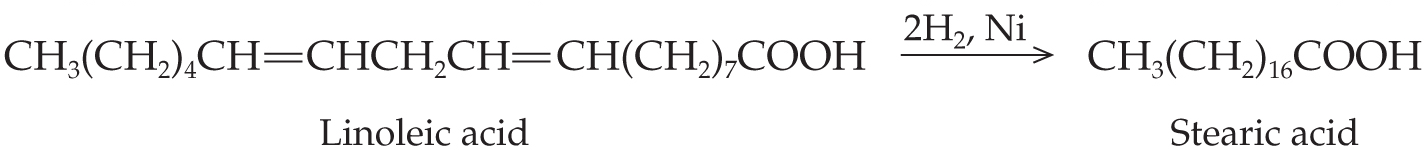
\includegraphics[width=0.7\linewidth]{hydrogenering}
	\caption[Hydrogenering]{Hydrogenering}
	\label{fig:hydrogenering}
\end{figure}
%Mooie samenvatting op slide 16
\subsection{Glyceriden}
\subsubsection{Structuur}
Glyceriden zijn lipide-esters, dit wil zeggen dat de alcoholgroep van glycerol een ester vormt met een vetzuur (zie figuur \ref{fig:structuurglyceriden}). Deze estervorming kan zich op één, twee of alle 3 de alcoholgroepen van de glycerol voordoen. We spreken van mono-, di-, triglyceriden.
\begin{figure}[h]
	\centering
	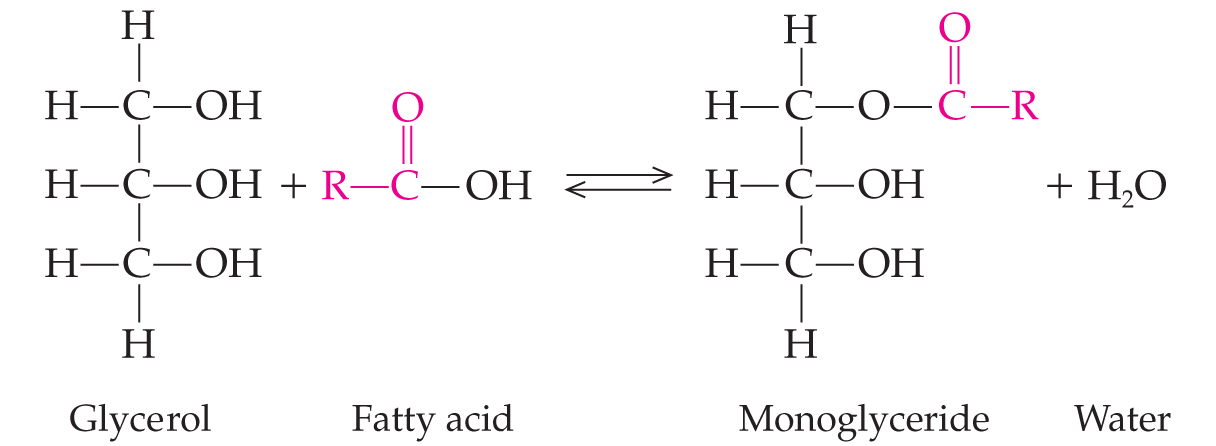
\includegraphics[width=0.6\linewidth]{structuur_glyceriden}
	\caption[Structuur glyceriden]{Structuur glyceriden}
	\label{fig:structuurglyceriden}
\end{figure}

\subsubsection{Triglyceriden}
Triglyceriden zijn non-ionische en niet polaire moleculen (zie figuur \ref{fig:triglyceride}) die dienen als energieopslag in vetcellen. Het zijn de meest voorkomende neutrale glyceriden in de natuur. Ze zijn bij vissen en planten vloeibaar bij kamertemperatuur dankzij de grote hoeveelheid onverzadigde vetzuren die aanwezig zijn. Bij mens en dier zijn de vetzuren hoofdzakelijk verzadigd, en dus zijn de triglyceriden ook vast bij kamertemperatuur.
\begin{figure}[h]
	\centering
	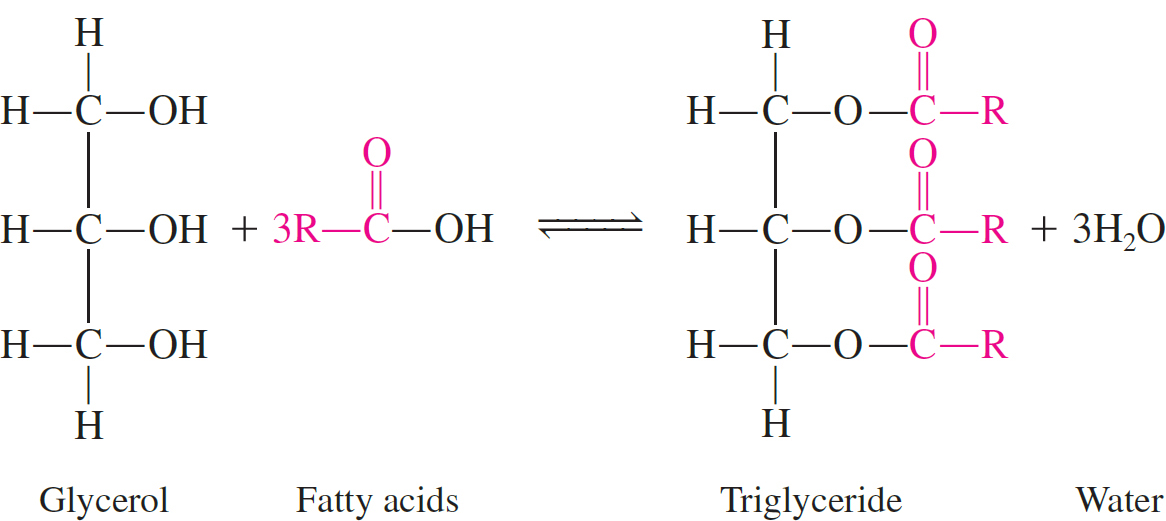
\includegraphics[width=0.6\linewidth]{Triglyceride}
	\caption[Triglyceride]{Triglyceride}
	\label{fig:triglyceride}
\end{figure}
\subsubsection{Reacties}
\textbf{Hydrolyse}\\
Produceert de vetzuren en glycerol. Het breekt dus eigenlijk een mono-, di-, triglyceride af tot zijn basiscomponenten (zie figuur \ref{fig:hydrolyseglyceriden}).
\begin{figure}[h]
	\centering
	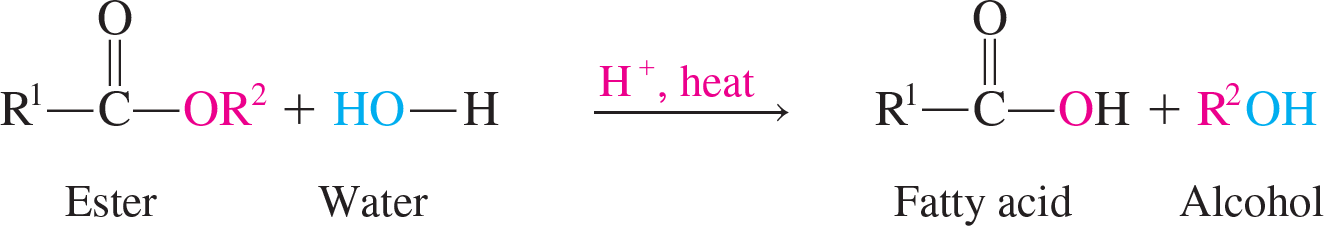
\includegraphics[width=0.7\linewidth]{HydrolyseGlyceriden}
	\caption[Hydrolyse]{Hydrolyse}
	\label{fig:hydrolyseglyceriden}
\end{figure}\\
\textbf{Verzeping}\\
Produceert vetzuurzouten en glycerol (zie figuur \ref{fig:verzepingglyceriden}).
\begin{figure}[h]
	\centering
	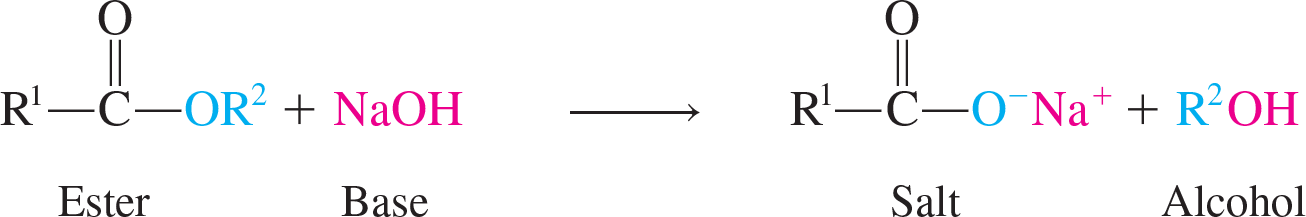
\includegraphics[width=0.7\linewidth]{VerzepingGlyceriden}
	\caption[Verzeping]{Verzeping}
	\label{fig:verzepingglyceriden}
\end{figure}
 \newpage
\subsubsection{Fosfoglyceriden}
Fosfoglyceriden zijn niet-neutrale glyceriden die opgemaakt zijn uit glycerol, vetzuur en een fosfaat-groep waarop eventueel nog andere groepen gebonden zijn zoals in figuur \ref{fig:fosfoglyeride}. De functie ervan zal later aan bod komen in het hoofdstuk over cellen. 
\begin{figure}[h]
	\centering
	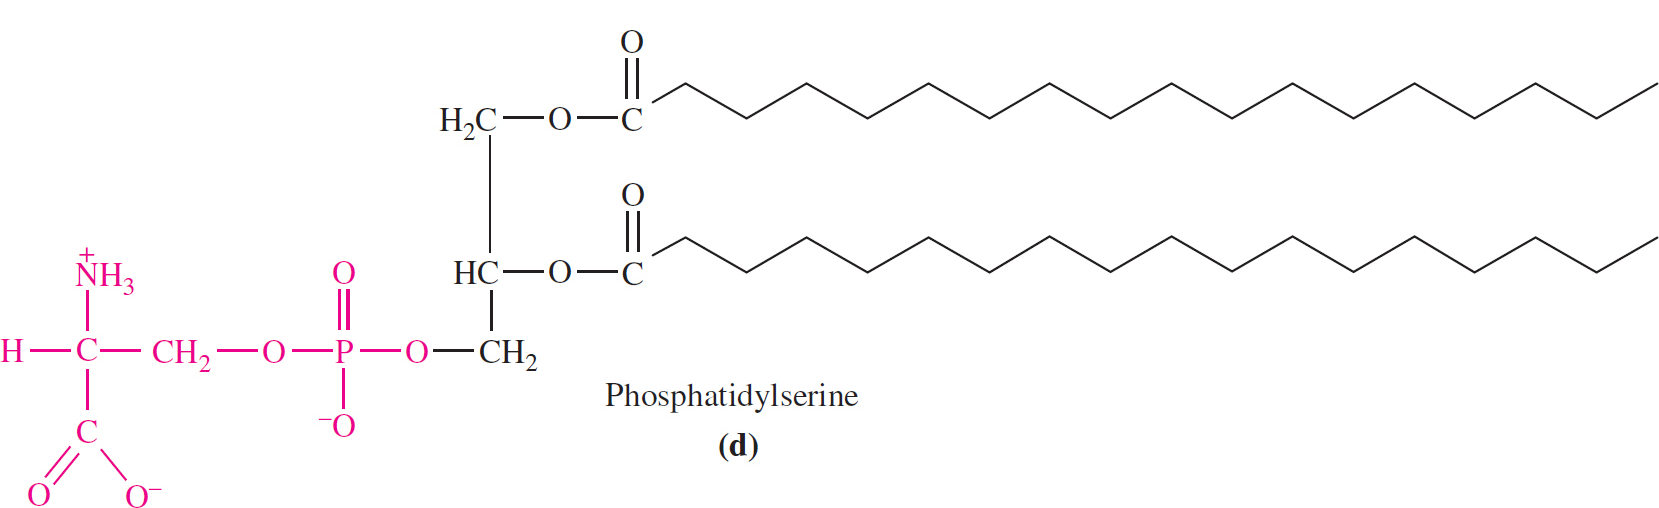
\includegraphics[width=0.7\linewidth]{fosfoglyeride}
	\caption[Fosfoglyceride]{Fosfoglyceride}
	\label{fig:fosfoglyeride}
\end{figure}

\subsection{Niet-glyceride lipiden}
\subsubsection{Sfingolipide}
Sfingolipiden worden getypeerd door hun sfingosine ruggengraat (zie figuur \ref{fig:sfingolipide}). Hieraan kunnen verschillende groepen binden, zoals vetzuren, fosfaat of koolhydraten. Men vind deze moleculen vooral terug in het celmembraan. 
\begin{figure}[h]
	\centering
	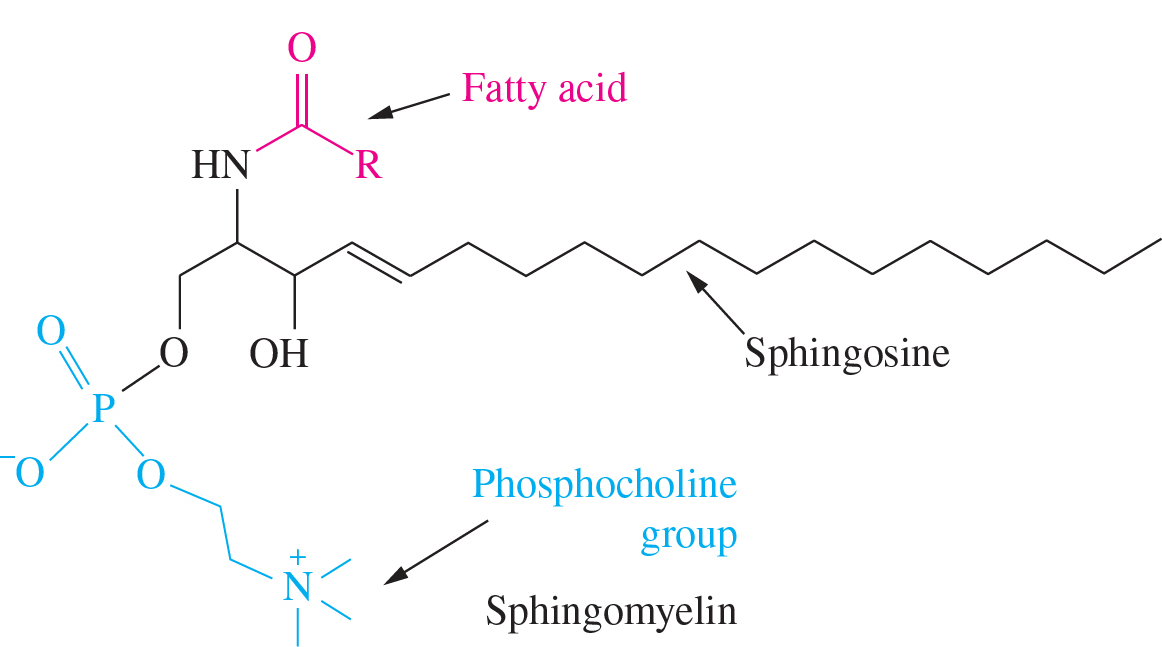
\includegraphics[width=0.5\linewidth]{sfingolipide}
	\caption[Sfingolipide]{Sfingolipide}
	\label{fig:sfingolipide}
\end{figure}
\subsubsection{Steroïden}
Steroïden volgen de algemene structuur die te zien is in figuur \ref{fig:steroidenstructuur}. 
\begin{figure}[h]
	\centering
	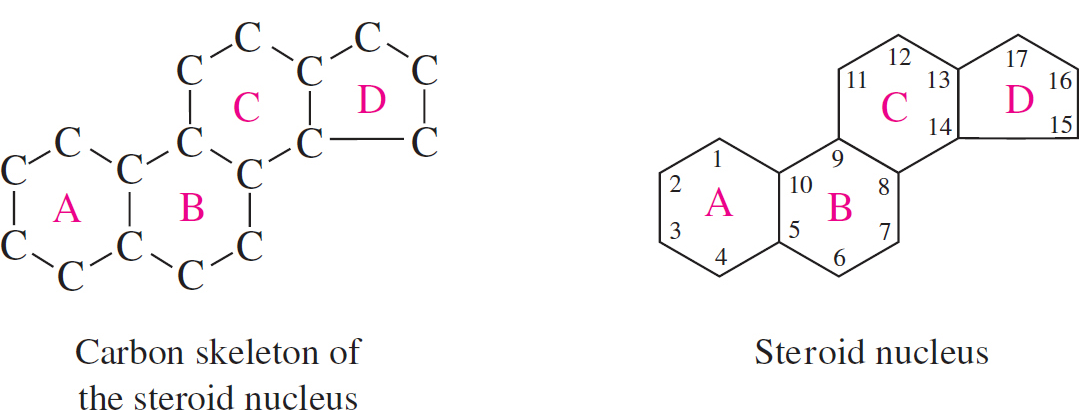
\includegraphics[width=0.5\linewidth]{steroidenstructuur}
	\caption[steroïden]{Steroïden}
	\label{fig:steroidenstructuur}
\end{figure}\\
Cholesterol is een belangrijke steroïde die we nodig hebben om galzouten, hormonen en vitaminen aan te maken. Zoals altijd is een balans wel belangrijk, te veel cholesterol kan leiden tot het dichtslippen van aders. 

\section{Celstructuren}
\subsection{Microscopische observatie van cellen}
Cellen zijn bijna altijd te klein om met het blote oog te zien. Om deze levensvormen toch te zien maken we gebruik van microscopen. Hiervoor bestaan 2 varianten: de licht microscoop en de elektronen microscoop. 

De licht microscoop is een (relatief) goedkope optie. We maken ook nog onderscheid tussen de klassieke en digitale microscoop. Door de eigenschappen van licht, is er een limiet aan de resolutie waarmee we kunnen observeren. De elektronen microscoop lost dit probleem op door een bundel elektronen te gebruiken. We kunnen opnieuw 2 verschillende soorten onderscheiden, de TEM en de SEM. 
\subsection{Celtheorie}
We stellen dat alle organismen zijn samengesteld uit cellen. Deze cellen zijn ook altijd afkomstig van reeds bestaande cellen en zijn erg klein. De reden dat ze microscopisch klein zijn, is de oppervlakte-volume verhouding. Dit wil zeggen dat kleine cellen een relatief grote oppervlakte hebben in vergelijking met hun volume. Aangezien cellen hun wand gebruiken voor het uitwisselen van stoffen, is het dus voordelig om een relatief groot wand oppervlak te hebben. Er zijn nog andere mogelijkheden om de oppervlakte te vergroten, zo maken enkele cellen microvilli aan zoals te zien in figuur \ref{fig:microvilli}.
\begin{figure}[h]
	\centering
	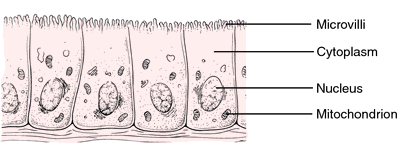
\includegraphics[width=0.7\linewidth]{Microvilli}
	\caption[Microvilli]{Microvilli}
	\label{fig:microvilli}
\end{figure}
\newpage
\subsection{Plasmamembraan}
Het plasmamembraan markeert de grens tussen buiten- en binnenkant een cel. Het is essentieel voor transport van stoffen in en uit de cel. Een plasmamembraan is opgebouwd uit een fosfolipide dubbellaag met ingebouwde eiwitten. Hierbij is de polaire (en dus hydrofiele) zijde van de fosfolipiden gericht naar het waterig medium. De niet-polaire staarten (hydrofoob) staan tegenover elkaar (zie figuur \ref{fig:plasmamembraan}). Als geheel vormen ze ook een vloeistofmozaïekmodel. Dit model zorgt ervoor dat het membraan extreem flexibel is. 
\begin{figure}[h]
	\centering
	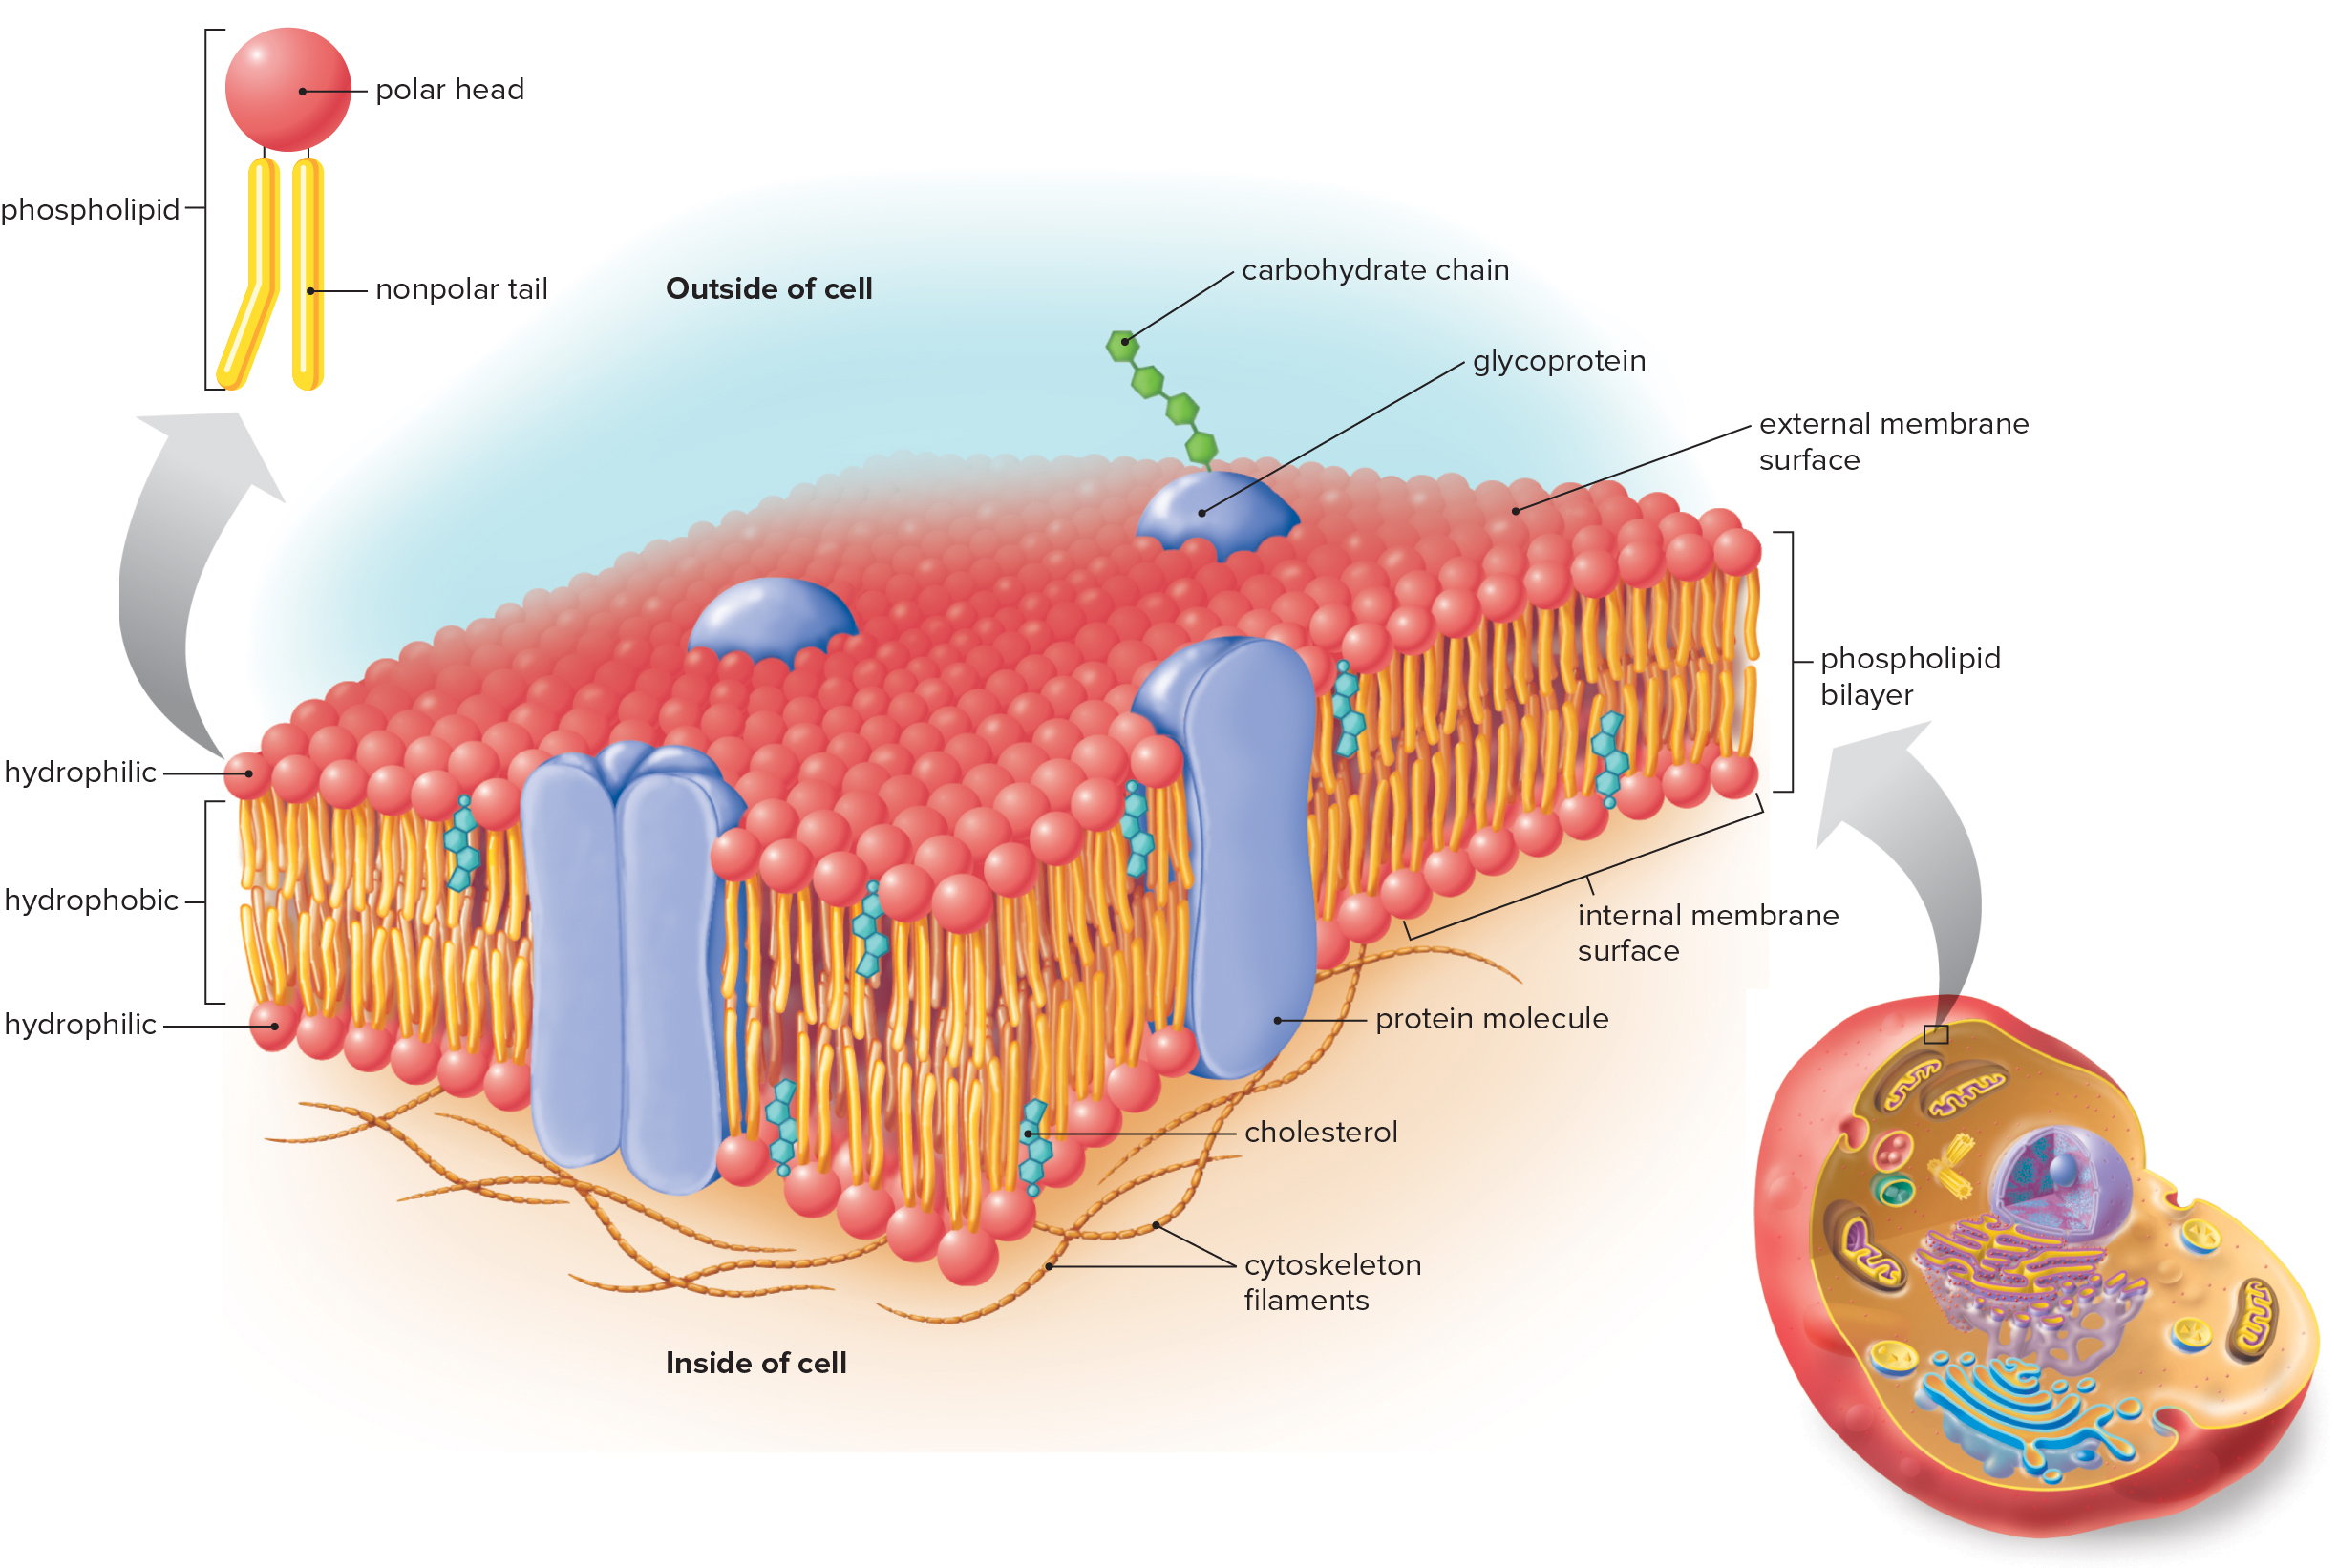
\includegraphics[width=0.8\linewidth]{Plasmamembraan}
	\caption[Plasmamembraan]{Plasmamembraan}
	\label{fig:plasmamembraan}
\end{figure}

Afhankelijk van de omstandigheden waarin de cel zich bevindt, kan de structuur van de vetzuren veranderen. In koude klimaten zullen er meer onverzadigde vetzuren aanwezig zijn, hierdoor dal de vloeibaarheid van het membraan stijgen. Het omgekeerde geldt voor cellen in warme omstandigheden. 

Membraan proteïnen zijn niet alleen belangrijk voor de communicatie van de cel, maar ook voor nutriëntenopname en afvalverwijdering. We onderscheiden 6 verschillende soorten proteïnen. Kanaalproteïnen (figuur \ref{fig:kanaal}) worden hoofdzakelijk gebruikt om specifieke moleculen door de celmembraan te loodsen; transportproteïnen (figuur \ref{fig:transport})zijn dan weer betrokken bij de doorgang van moleculen door het membraan, waarbij soms input van energie nodig is. Celherkenningsproteïnen worden gebruikt om een onderscheid te maken tussen cellen van ons eigen lichaam, en die van andere organismen (figuur \ref{fig:Celherkenningsproteïnen}). Receptorproteïnen laten signaalmoleculen toe om te binden, hierdoor ontstaat een cellulaire respons (figuur \ref{fig:Receptorproteïnen}). Enzymatische proteïnen katalyseren metabole reacties (figuur \ref{fig:Enzymproteïnen}). Tot slot worden junctie-proteïnen gebruikt om verbindingen te vormen tussen cellen, hierbij is cel-tot-cel hechting en communicatie mogelijk (figuur \ref{fig:Junctieproteïnen}).
\begin{figure}[!htbp]
	\centering
	\begin{subfigure}{.5\textwidth}
		\centering
		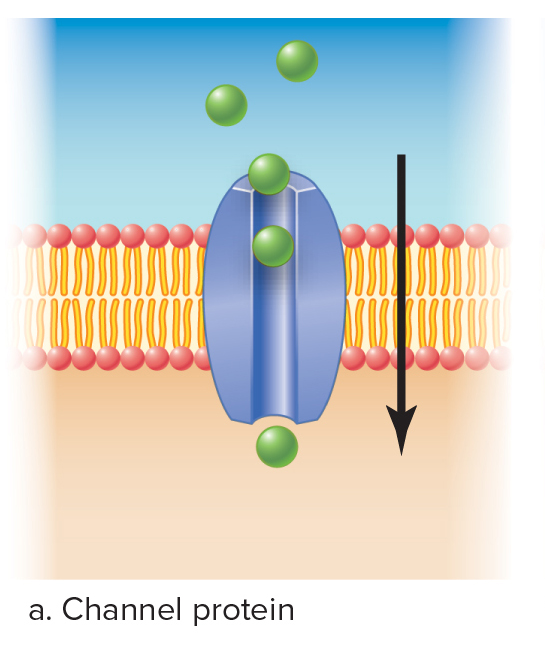
\includegraphics[width=0.7\linewidth]{Kanaalprot}
		\caption{Kanaalproteïnen}
		\label{fig:kanaal}
	\end{subfigure}%
	\begin{subfigure}{.5\textwidth}
		\centering
		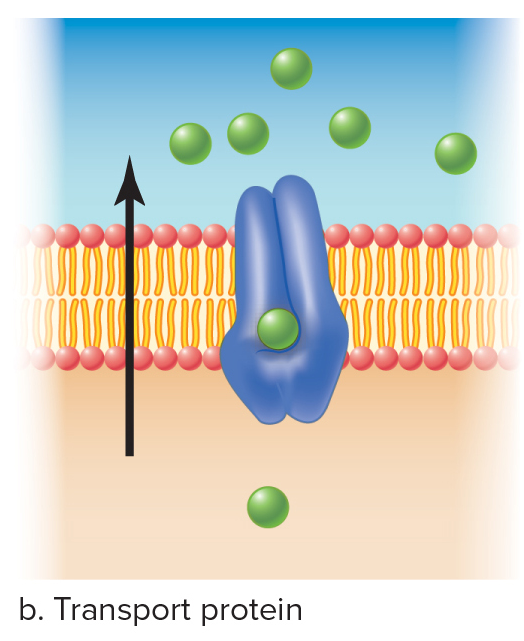
\includegraphics[width=0.7\linewidth]{transportprot}
		\caption{Transportproteïnen}
		\label{fig:transport}
	\end{subfigure}
\medskip
	\begin{subfigure}{.5\textwidth}
		\centering
		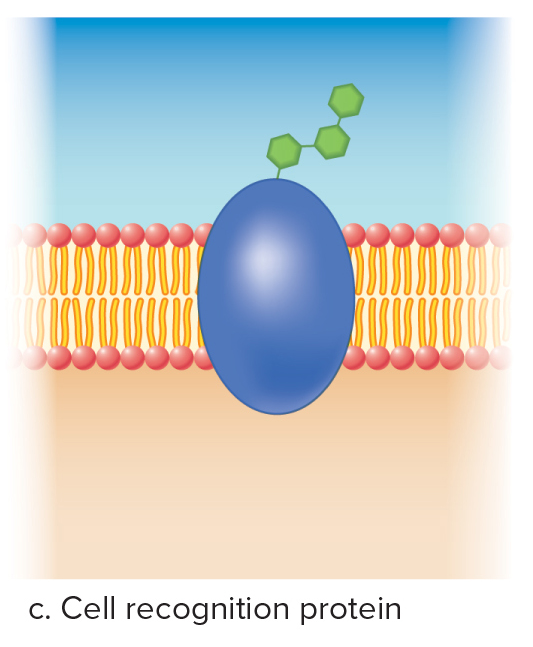
\includegraphics[width=0.7\linewidth]{Celherkenningsprot}
		\caption{Celherkenningsproteïnen}
		\label{fig:Celherkenningsproteïnen}
	\end{subfigure}%
	\begin{subfigure}{.5\textwidth}
		\centering
		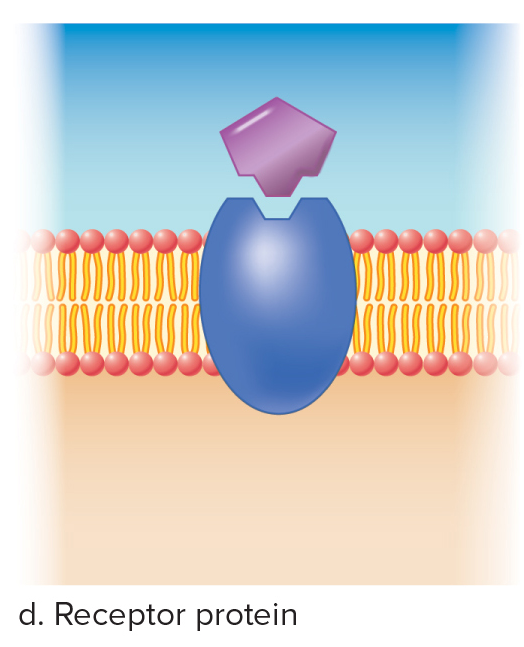
\includegraphics[width=0.7\linewidth]{Receptorprot}
		\caption{Receptorproteïnen}
		\label{fig:Receptorproteïnen}
	\end{subfigure}
\medskip
	\begin{subfigure}{.5\textwidth}
		\centering
		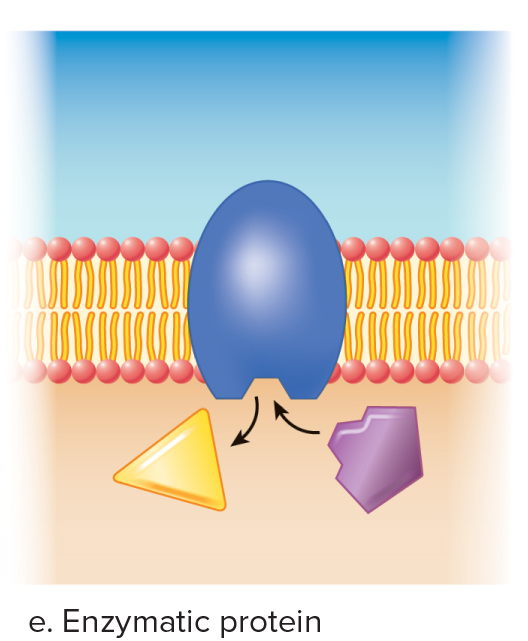
\includegraphics[width=0.7\linewidth]{Enzymatischeprot}
		\caption{Enzymatische proteïnen}
		\label{fig:Enzymproteïnen}
	\end{subfigure}%
	\begin{subfigure}{.5\textwidth}
		\centering
		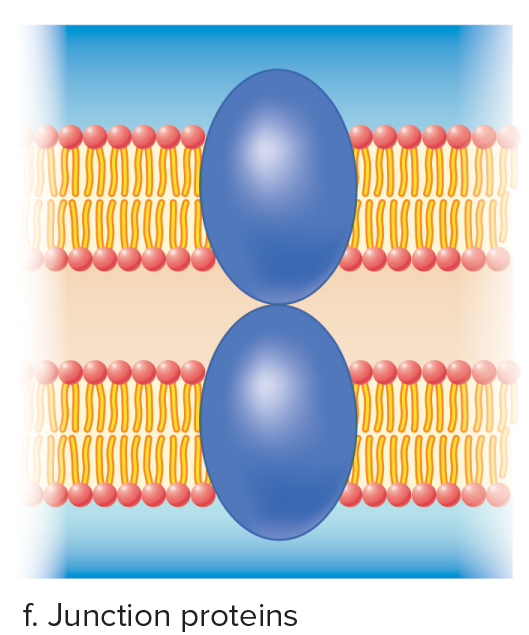
\includegraphics[width=0.7\linewidth]{Junctieprot}
		\caption{Junctie-proteïnen}
		\label{fig:Junctieproteïnen}
	\end{subfigure}
	\caption{Membraanproteïnen}
	\label{fig:membraanprot}
\end{figure}\\
\newpage
\subsection{2 types cellen}
We definiëren twee types cellen op basis van de organisatie van genetisch materiaal. Eukaryote cellen hebben membraanomringd DNA, de celkern. Bij de prokaryote cellen ontbreekt deze structuur.  
\subsubsection{Prokaryote cellen}
Het zijn eencellige organismen die uit de bacteria en archaea domeinen komen. Over het algemeen zijn het kleine en vrij eenvoudige organismen. Hierdoor zijn ze wel in staat om snel en effectief te reproduceren. Ze zijn hierdoor ook een zeer diverse groep organismen. 

Bacteriën zijn bekende prokaryote cellen. Ze kunnen bij de mens verschillende ziektes veroorzaken, maar ze hebben ook voordelen. We gebruiken ze om chemicaliën, voedsel en geneesmiddelen te produceren. 

De structuur van prokaryote cellen kan sterk verschillen, hier nemen we het voorbeeld van een bacterie. zoals te zien is in figuur \ref{fig:prokaryotecellen}, hebben we cytoplasma dat omringd is door een plasmamembraan en celwand. Bij sommige bacteriën kan deze celwand echter niet aanwezig zijn. Er is ook een mogelijkheid op een beschermende capsule. De celwand is verantwoordelijk voor het behoud van de vorm van de cel. Het cirkelvormig dubbelstrengig DNA bevindt zich in het nucleoid zonder omringend membraan. Er zijn ook andere celstructuren aanwezig die later besproken worden.
 

\begin{figure}[h]
	\centering
	\includegraphics[width=0.7\linewidth]{Prokaryote_cellen}
	\caption[Prokaryote cel]{Prokaryote cel}
	\label{fig:prokaryotecellen}
\end{figure}
\newpage
\subsubsection{Eukaryote cellen}
Dit zijn vaak dierlijke cellen, ze maken dus een deel uit van een multicellulair organisme. Soms komen ze ook vaak als micro-organismen, deze kunnen multicellulair zijn, maar kunnen ook unicellulair zijn zoals bijvoorbeeld gist. Ook algen bestaan uit eukaryote cellen. In het algemeen zijn dit complexere levensvormen (zie figuur \ref{fig:eukaryotecel}). De aanwezige celstructuren worden besproken in subsectie \ref{sec:IntracellulaireStructuren}. 
\begin{figure}[h]
	\centering
	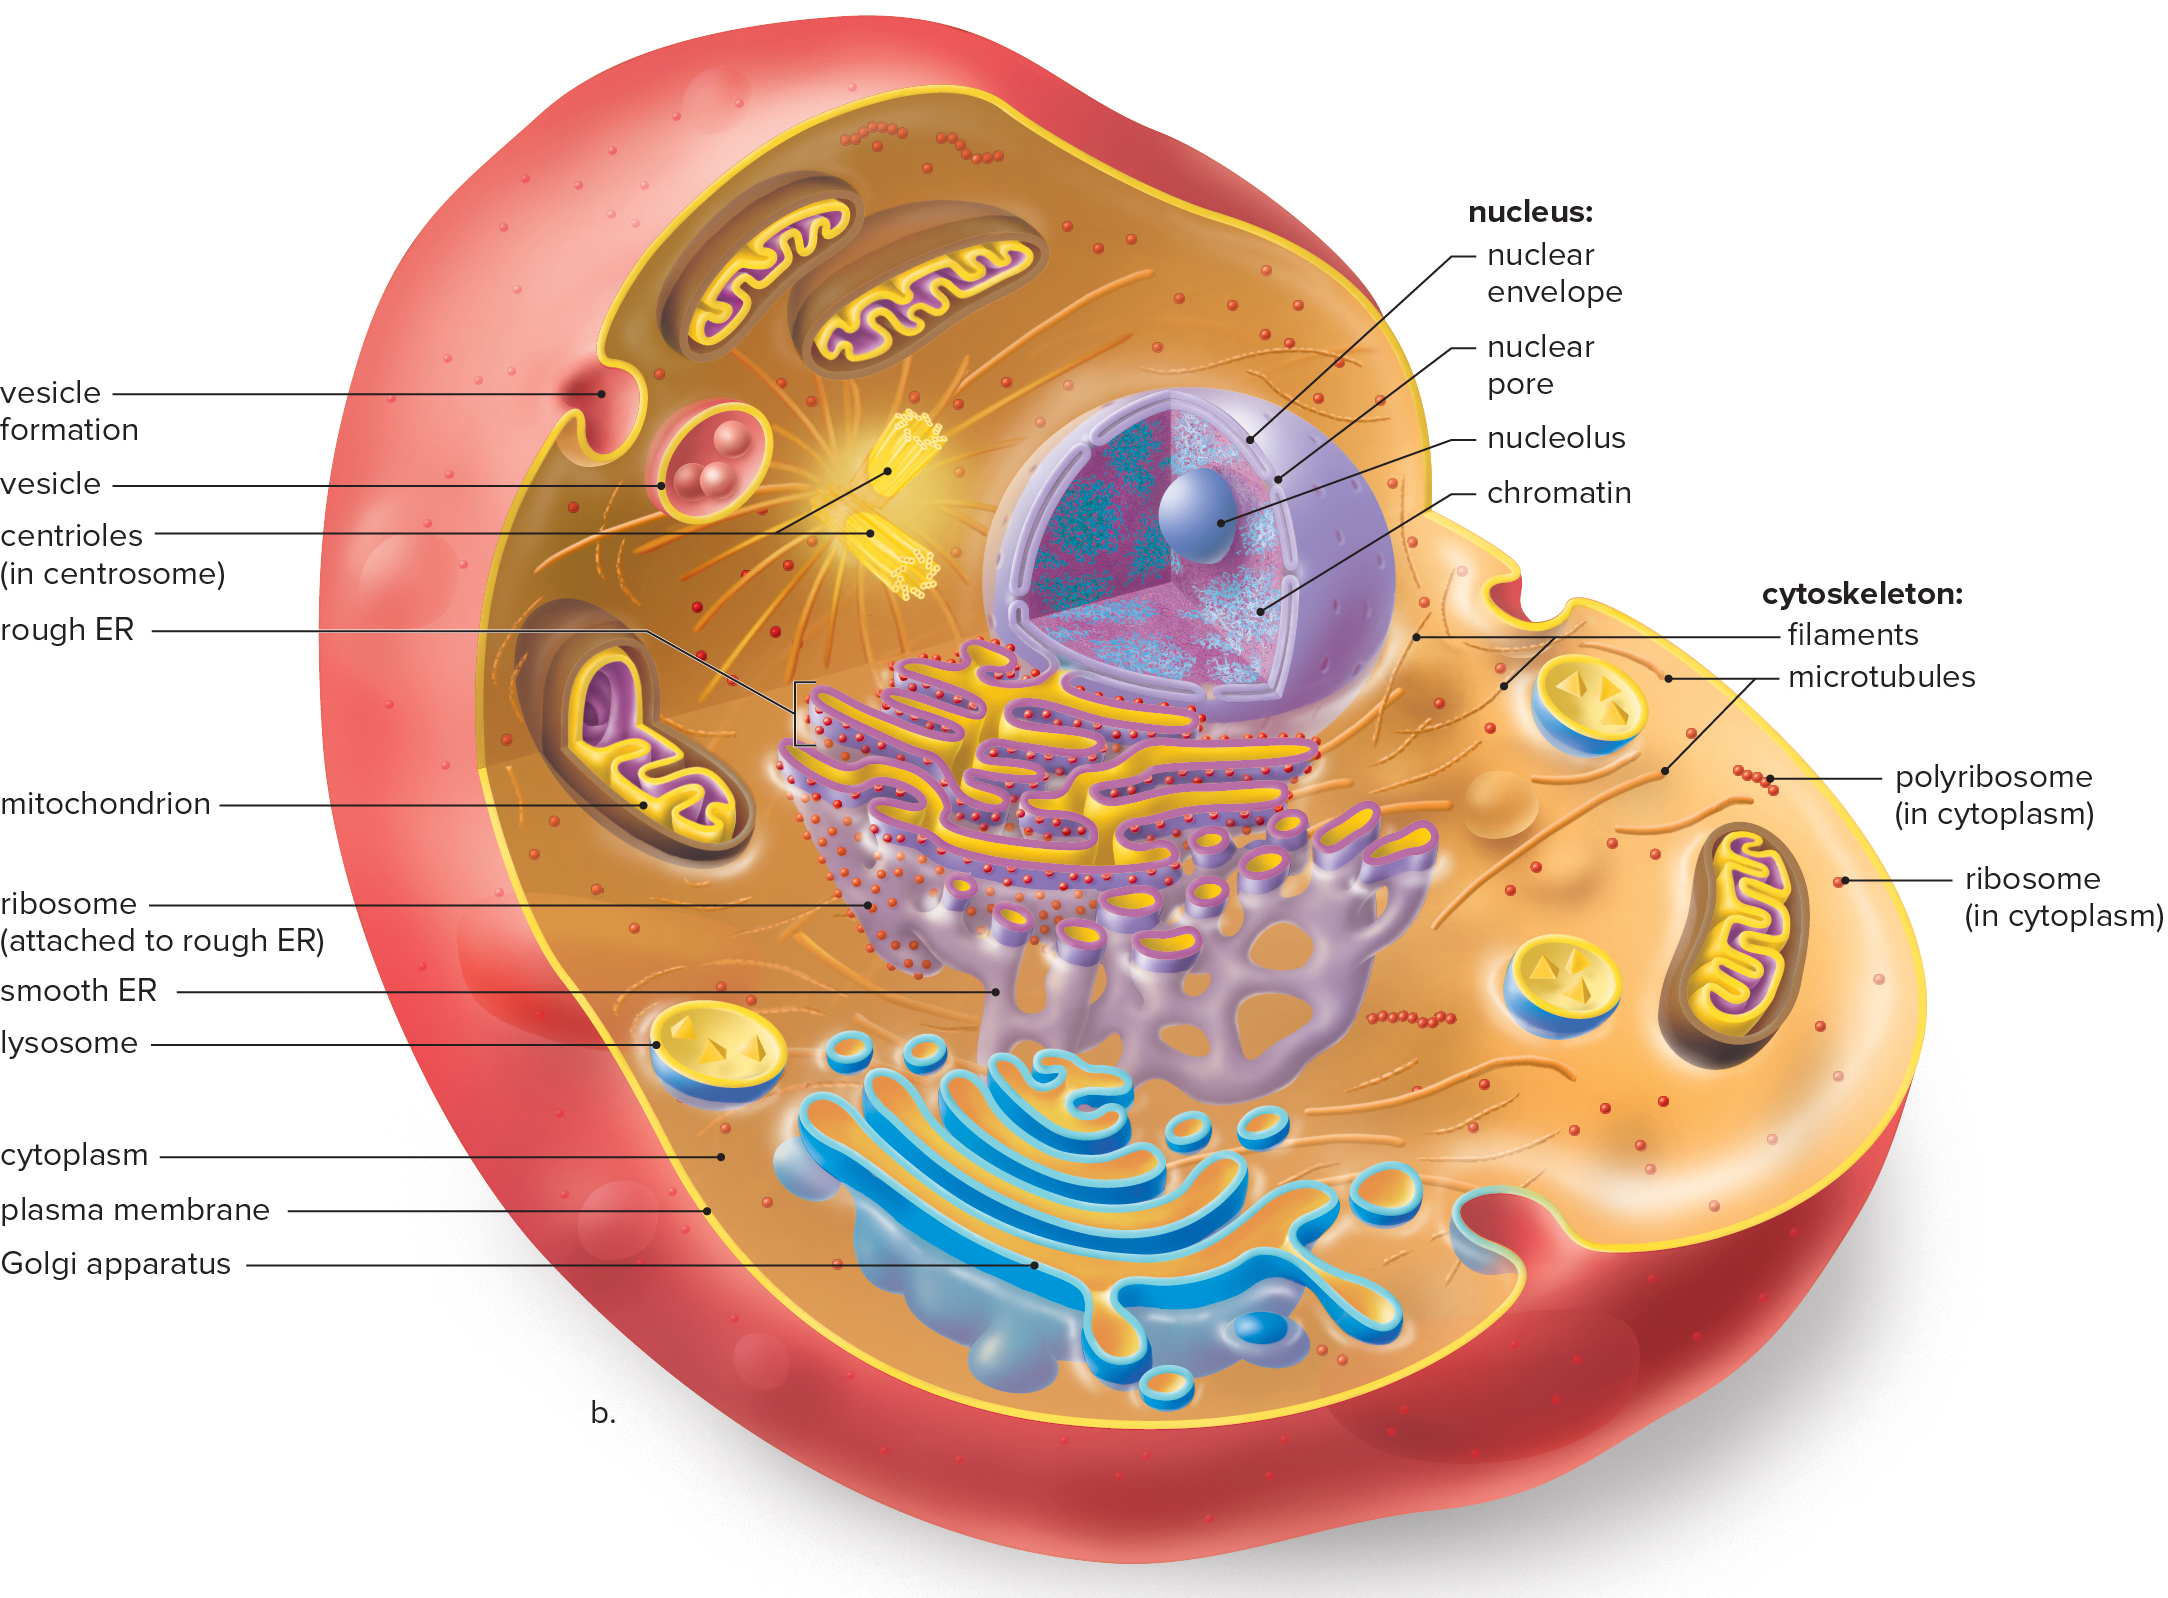
\includegraphics[width=0.5\linewidth]{Eukaryote_cel}
	\caption[Eukaryote cel]{Eukaryote cel}
	\label{fig:eukaryotecel}
\end{figure}

\subsection{Intracellulaire structuren}
\label{sec:IntracellulaireStructuren}
\subsubsection{Nucleus}
De nucleus (zie figuur \ref{fig:nucleus}) oftewel de celkern is een nucleaire envelop gemaakt uit een dubbel membraan. Nucleaire poriën zorgen voor transport van stoffen in en uit de kern. De belangrijkste taak van de celkern is om genetische informatie op te slaan. Dit gebeurt met chromatine, een soort geheel van DNA, proteïne en RNA (Voor celdeling zal het DNA zich condenseren in lineaire chromosomen). DNA met informatie in genen zal een transcriptie krijgen naar messengerRNA oftewel mRNA. Dit proces gebeurt buiten de celkern in het cytoplasma, met behulp van ribosomen wordt mRNA dan vertaald in polypeptiden. De nucleolus is de regio waar ribosomaalRNA oftewel rRNA wordt aangemaakt.
\begin{figure}[h]
	\centering
	\includegraphics[width=0.5\linewidth]{Nucleus}
	\caption[Nucleus]{Nucleus}
	\label{fig:nucleus}
\end{figure}

\subsubsection{Ribosomen}
Ribosomen (figuur \ref{fig:ribosoom}) zijn verantwoordelijk voor de eiwitsynthese, dit gebeurt in het cytoplasma. We vinden deze structuur in zowel prokaryote als eukaryote levensvormen. Een ribosoom is samengesteld uit twee subeenheden (verdere verduidelijking in sectie \ref{sec:dnabiologie}). Het ribosoom ontvangt mRNA en leest dit als instructiereeks van aminozuren in een polypeptide. In eukaryoten bewegen sommige ribosomen vrij rond in het cytoplasma maar de meeste zijn gehecht aan het endoplasmatisch reticulum. 
\begin{figure}[h]
	\centering
	\includegraphics[width=0.5\linewidth]{ribosoom}
	\caption[Ribosoom]{Ribosoom}
	\label{fig:ribosoom}
\end{figure}

\subsubsection{Endomembraansysteem}
Het endomembraansysteem bestaat uit de nucleaire envelop, endoplasmatisch reticulum, het Golgi apparaat en talrijke vesikels. Het zorgt voor compartmentalisering binnen een cel (beperkt tot bepaalde regio's). Vesikels zorgen voor transport van moleculen binnen in de cel.
\paragraph{Endoplasmisch reticulum}
Het endoplasmatisch reticulum (figuur \ref{fig:endoplasmatisch-reticulum}) is een complex systeem van membraan-kanalen en `zakjes'. Het is fysiek verbonden met de buitenste membraan van het nucleair-membraan. We kunnen 2 soorten reticulum onderscheiden, we beginnen met de ruwe variant. Het is bezaaid met ribosomen, en dient vooral voor de modificatie van eiwitten in lumen en vormt transportvesikels die naar het Golgi apparaat gaat. De gladde variant, is continu met het ruw endoplasmatisch reticulum, het bevat wel geen ribosomen.  Het dient vooral om stoffen zoals fosfolipiden en steroïden te synthetiseren. De exacte molecule die geproduceerd wordt is wel afhankelijk van het type cel.  
\begin{figure}[h]
	\centering
	\includegraphics[width=0.4\linewidth]{"Endoplasmatisch reticulum"}
	\caption[Endoplasmatisch reticulum]{Endoplasmatisch reticulum}
	\label{fig:endoplasmatisch-reticulum}
\end{figure}

\paragraph{Golgi apparaat}
Het Golgi apparaat kan het best vergeleken worden met een transfer station: het is verantwoordelijk voor de transfer van moleculen tussen het endoplasmatisch reticulum en andere vesikels (blaasjes). \\
Vesikels worden ontvangen uit het ruwe én gladde endoplasmatisch reticulum, ze worden binnenin gemodificeerd en verplaatst todat ze uiteindelijk gesorteerd en weggestuurd worden. De moleculen die het apparaat terug verlaten worden wederom in vesikels verpakt. Ze eindigen terug in het endoplasmatisch reticulum of het plasmamembraan. In dierlijke cellen zijn sommige van de vesikels lysosomen.  \\
Qua bouw is het Golgi apparaat een stapel afgeplatte zakjes. Net zoals glad endoplasmatisch reticulum bevat het apparaat geen ribosomen, maar het Golgi apparaat is wel compacter.
\paragraph{Lysosomen}
Lysosomen zijn vesikels die moleculen of delen van de cel verteren. Het zijn dus intracellulaire verteringsenzymen.
\subsubsection{Vacuole}
Een vacuole (figuur \ref{fig:vacuole})is een membraanzakje dat een stuk groter is dan vesikels. Het kan meerdere meerdere functies aan nemen binnen de cel: afvoer van overtollig water, vertering en opslag van plantpigmenten of vet.
\begin{figure}[!h]
	\centering
	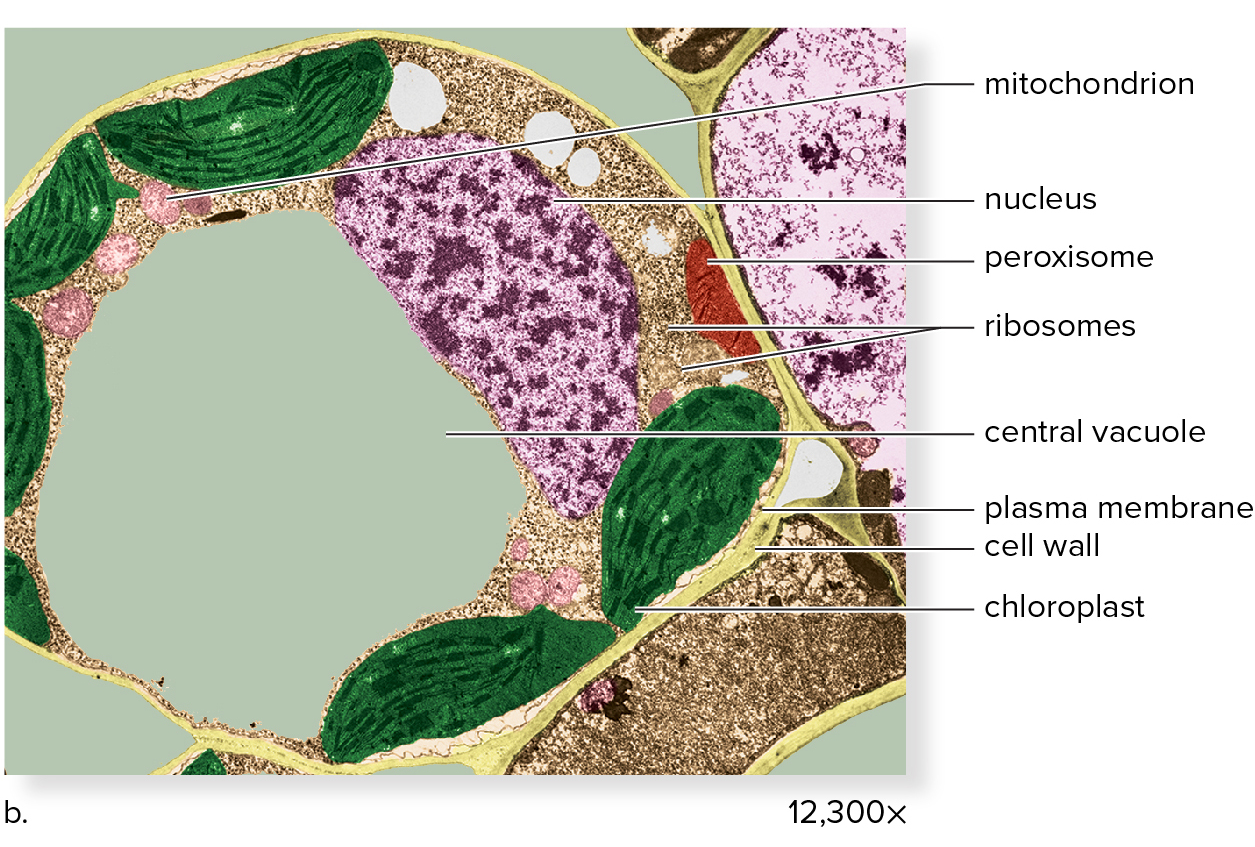
\includegraphics[width=0.5\linewidth]{Vacuole}
	\caption[Vacuole]{Vacuole}
	\label{fig:vacuole}
\end{figure}
\newpage
\subsubsection{Energie-organellen}
\paragraph{Mitochondriën}
Mitochondriën vinden we zowel in planten als dieren, ze zijn erg klein waardoor ze enkel te zien zijn met een elektronenmicroscoop. Ze hebben een dubbelmembraan waarbij de binnenste membraan een groter oppervlak heeft dan de buitenste. Dit betekend dat er plooien moeten komen in het binnenste membraan, deze plooien noemen we cristae. Binnenin zit de matrix, dit bevat enzymen die koolhydraatafbraak ondersteunen, om dan ATP te synthetiseren. Verdere functies van Mitochondriën worden verduidelijkt in sectie \ref{sec:energie}.
\begin{figure}[h!]
	\centering
	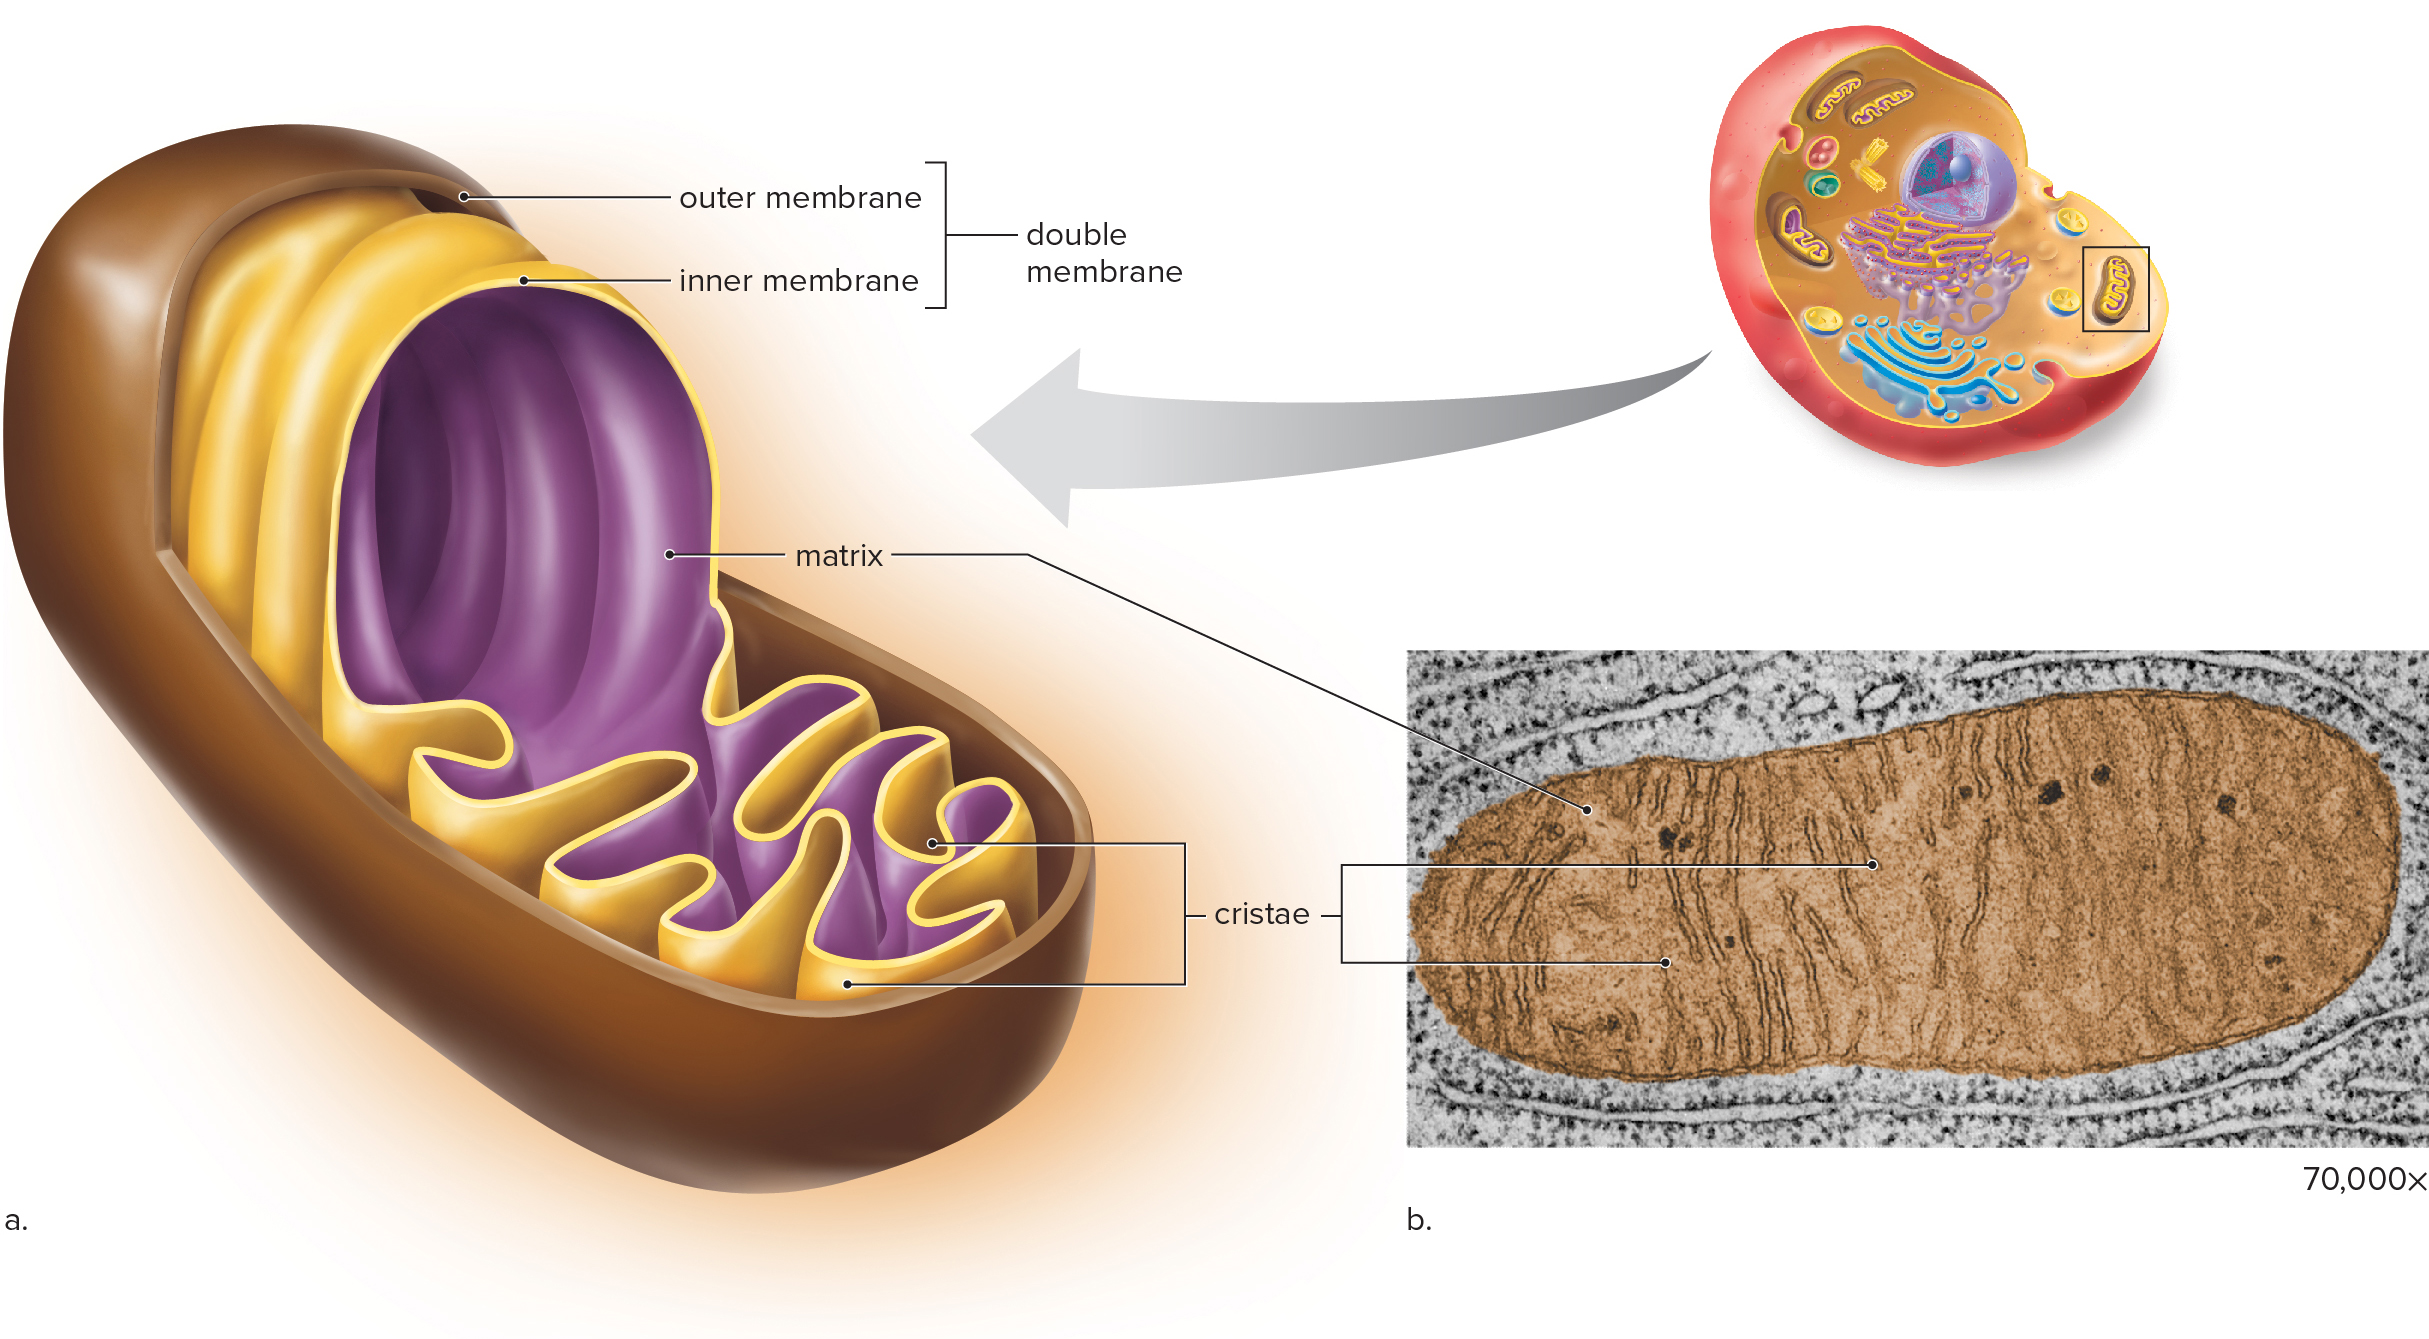
\includegraphics[width=0.7\linewidth]{PowerhouseOfTheCell}
	\caption[Mitochondria]{Mitochondriën: The Powerhouse of The Cel!}
	\label{fig:powerhouseofthecell}
\end{figure}
\paragraph{Chloroplasten}
Dit celorganel gebruikt zonne-energie om koolhydraten aan te maken via het fotosynthese-proces. We vinden de chloroplast terug in planten en algen. Het bestaat uit 3 membraansystemen, eerst en vooral hebben we een dubbelmembraan die het stroma omhult. Het derde membraan vormt de thylakoiden. Deze bevatten het pigment om zonlicht op te vangen. Chloroplasten hebben hun eigen DNA en ribosomen.  
\begin{figure}[h]
	\centering
	\includegraphics[width=0.7\linewidth]{Chloroplast}
	\caption[Chloroplast]{Chloroplast}
	\label{fig:chloroplast}
\end{figure}
\newpage
\subsubsection{Cytoskelet}
Het cytoskelet is opgebouwd uit proteïnen en vormt een netwerk van onderling verbonden proteïnenfilamenten. Het strekt zich uit van de kern tot aan het plasmamembraan, en wordt meestal enkel gevonden in eukaryote cellen. Een cytoskelet zorgt voor behoud van vorm in de cel.
\begin{figure}[h]
	\centering
	\includegraphics[width=0.5\linewidth]{Cytoskelet}
	\caption[Cytoskelet]{Cytoskelet}
	\label{fig:cytoskelet}
\end{figure}\\
Als we verder inzoomen op het cytoskelet, zien we dat het opgebouwd is uit microtubuli. Het zijn kleine, holle cilinders die de vorm van de cel grotendeels bepalen. De synthese hiervan wordt gecontroleerd door het centrosoom. De microtubuli zorgen voor behoud van de cel-vorm en fungeren als transportbaan voor organellen en andere materialen. Het geheel is dynamisch: de lengte wordt eenvoudig aangepast afhankelijk van waar in de cel stoffen afgeleverd moeten worden. 
Naast de microtubuli zijn er de intermediaire filamenten en actine filamenten. De intermediaire filament bieden net zoals de microtubuli stevigheid via een netwerk tussen de celkern en de plasmamembraan. Het grootste verschil met microtubuli is dat de intermediaire filamenten veel minder dynamisch zijn.
Tot slot zijn er de actine filamenten. Ze vormen en dens netwerk net onder het plasmamembraan. Door het afbreken aan één kant en terug opbouwen aan de andere kant, zorgen zij voor de bewegelijkheid van een cel.

\subsubsection{Centriolen}
Een centriool is gemaakt van negen sets microtubuli tripletten. In de cel liggen twee centriolen loodrecht op elkaar, zij vormen het centrosoom. We vinden deze structuren enkel in dierlijke cellen, niet in plantencellen. Ze zijn verantwoordelijk voor het organiseren van microtubuli tijdens de celdeling. 
\begin{figure}[h]
	\centering
	\includegraphics[width=0.5\linewidth]{Centriolen}
	\caption[Centriolen]{Centriolen}
	\label{fig:centriolen}
\end{figure}
\newpage
\subsubsection{Cilia en flagellen}
We vinden cilia en flagellen (figuur \ref{fig:ciliaenflagellen}) in eukaryote levensvormen. Ze zijn essentieel voor beweging van de cel of de vloeistoffen rond de cel. Beiden zijn vergelijkbaar in opbouw, namelijk een 9+2 patroon van microtubuli. De cilia zijn wel korter (maar talrijker) dan flagellen.
\begin{figure}[h]
	\centering
	\includegraphics[width=0.7\linewidth]{Cilia_en_Flagellen}
	\caption[Cilia en flagellen]{Cilia en flagellen}
	\label{fig:ciliaenflagellen}
\end{figure}

\subsection{Extracellulaire structuren}
\subsubsection{Celwand}
De celwand biedt ondersteuning aan veel niet-dierlijke cellen zoals planten, schimmels en protisten. Er zijn ook bacteriën die een celwand hebben, maar dit is een andere structuur. De planten-celwand kent  altijd een primaire celwand. Deze bestaat uit cellulose fibrillen en andere polymeren. Deze wand rekt als de cel groeit. Sommige cellen hebben ook nog een secundaire wand die vormt binnen de primaire celwand. We vinden deze structuur bij houtige planten. De tweede wand voegt lignine toe aan de mix, dit component geeft extra kracht en bescherming. Cellen kunnen verbonden worden door plasmodesmata. Dit zijn kanalen die door de celwand gaan om zo de uitwisseling van water en kleine moleculen mogelijk te maken.
\subsubsection{Extracellulaire matrix}
De extracellulaire matrix (ECM) vinden we in dierlijke cellen, dit te vervanging van de celwand. Het is opgebouwd uit een complex netwerk van proteïnen en polysachariden, voorbeelden hiervan zijn collageen en elastine. Er bestaan meerdere types van deze matrix, zo kunnen we flexibel kraakbeen maken en relatief hard bot. 
\subsubsection{Juncties tussen cellen}
Adhesie juncties (figuur \ref{fig:Adhesie}) hebben interne cytoplasmatische structuren verbonden door intercellulaire filamenten. Het zijn stevige maar flexibele verbindingen tussen cellen. `Tight' juncties (figuur \ref{fig:Tight}) zijn lekdichte verbindingen tussen cellen. Tot slot zijn gap juncties (figuur \ref{fig:Gap}) de juncties die zorgen voor communicatie tussen twee aanliggende cellen. Het zijn kanalen doorheen de plasmamembranen.   

\begin{figure}[h]
	\centering
	\begin{subfigure}{.33\textwidth}
		\centering
		\includegraphics[width=1\linewidth]{Adhesie_Junctie}
		\caption{Adhesion Junction}
		\label{fig:Adhesie}
	\end{subfigure}%
	\begin{subfigure}{.33\textwidth}
		\centering
		\includegraphics[width=0.7\linewidth]{Tight_Junctie}
		\caption{Tight Junction}
		\label{fig:Tight}
	\end{subfigure}%
	\begin{subfigure}{.33\textwidth}
	\centering
	\includegraphics[width=0.7\linewidth]{Gap_Junctie}
	\caption{Gap Junction}
	\label{fig:Gap}
	\end{subfigure}
	\caption{Verschillende soorten juncties}
	\label{fig:Juncites}
\end{figure}
\subsection{Cellulaire reproductie}
Bij prokaryote cellen kennen we binaire splitsing (figuur \ref{fig:binairesplitsing}). Eukaryote cellen kennen 2 manieren van reproductie, het meiose proces wat meestal bij seksuele reproductie voorkomt. Het mitose proces is veel vaker gebruikt om een kloon te maken van de cel. We zien dat dit in een soort cyclus gebeurt (figuur \ref{fig:celcyclus}). Dit proces wordt sterk gecontroleerd in ons lichaam, als er te weinig mitose is worden cellen niet meer vervangen. Te veel mitose zorgt daarentegen voor cellen die ongecontroleerd reproduceren, wat de voorbode is voor tumors en kankers.  

\begin{figure}[h]
	\centering
	\begin{subfigure}{.5\textwidth}
		\centering
		\includegraphics[width=0.7\linewidth]{Celcyclus}
		\caption{Mitose celcyclus}
		\label{fig:celcyclus}
	\end{subfigure}%
	\begin{subfigure}{.5\textwidth}
		\centering
		\includegraphics[width=0.7\linewidth]{Binaire_Splitsing}
		\caption[Splitsing]{Binaire splitsing}
		\label{fig:binairesplitsing}
	\end{subfigure}
	\caption{Celreproductie}
	\label{fig:reproductie}
\end{figure}

\subsection{Wat met virussen?}
We zien virussen eigenlijk niet als levende organismen. Dit komt omdat ze niet opgebouwd zijn volgens normale cellen. Het kan zichzelf niet voortbewegen of zelfs voortplanten (een virus heeft een gastheercel nodig om zich voort te planten). Er is zelfs geen metabolisme aanwezig in een virus, we zien ze dus als dood materiaal. Er zijn enkele onderdelen die we herkennen bij alle virussen: we zien altijd een buitenste capside die samengesteld is uit proteïnen. Binnenin is er DNA of RNA aanwezig, het viraal genoom is zeer klein en kan verschillende vormen aan nemen. We kunnen over het algemeen ook stellen dat ze kleiner zijn dan andere cellen (we hebben een elektronen microscoop nodig om ze te zien). Sommige virussen hebben ook nog spikes voor de aanhechting met de gastheercel, er kan ook een enveloppe aanwezig zijn. 
\newpage
\section{Cases in rode biotechnologie}
\subsection{Wat is rode biotechnologie}
Rode biotechnologie gaat over de medische toepassingen die mogelijk gemaakt worden door onderzoek naar biotechnologie. Enkele voorbeelden zijn tests, ontwikkeling van geneesmiddelen en ontwikkeling van vaccins. 
\subsubsection{Diagnostische tests}
Door ontwikkelingen in diagnostische tests, is het mogelijk om sneller en goedkoper ziektes en aandoeningen op te sporen. Een voorbeeld hiervan is biomarker detectie. Biomarkers zijn moleculen die makkelijk detecteerbaar zijn, en een sterke indicator zijn van een aanwezige ziekte of de gezondheidstoestand van het lichaam. PSA is een voorbeeld van een biomarker die gebruikt wordt bij het opsporen van prostaatkanker. Ook de NIPT test wordt vaak gebruikt bij het detecteren van genetische afwijkingen bij ongeboren baby's, via een simpele bloedafname bij de moeder (risicoloos) kunnen we een schatting maken van de gezondheid van de baby.
\subsubsection{Geneesmiddelenontwikkeling en gentherapie}
Door het toepassen van de `High throughput screening' (HTS) methode (figuur \ref{fig:hts}), is het mogelijk om geneesmiddelen te ontwikkelen. In dit proces beginnen we met onderzoek naar moleculen die potentieel gebruikt kunnen worden om bacteriën te doden. Er wordt een keuze gemaakt om enkele duizenden moleculen te testen. In deze tests worden de bacteriën samengebracht met 1 molecule om te zien of ze zullen sterven, dit is volledig geautomatiseerd. Alle stoffen die erin slagen om de bacterie te doden gaan naar de volgende stap. Hier testen we op toxiciteit bij mensen, dit gebeurd op vrijwel dezelfde manier maar dan met menselijke cellen in plaats van bacteriën. Alle stoffen die niet toxisch zijn voor menselijk weefsel, kunnen door gaan naar de tests op organismen. Hierbij wordt de stof eerst toe gediend aan gezonde dieren, om te zien wat de effecten zijn. We gaan dan stapsgewijs over naar dieren die besmet zijn met de bacterie. Als deze testen positief zijn, kunnen we over gaan naar menselijke testen. Indien ook deze een gunstig resultaat opleveren, hebben we een werkend medicijn gevonden. 
\begin{figure}[h]
	\centering
	\includegraphics[width=0.7\linewidth]{HTS}
	\caption[HTS]{Hight Throughput screening}
	\label{fig:hts}
\end{figure}

Door biotechnologie kunnen we ook bacteriën gebruiken om medicijnen mee te maken. Een voorbeeld hiervan is dat we insuline voor diabeten niet meer halen bij varkens, maar laten produceren door een bacterie. Meer hierover in sectie \ref{sec:dnaandgenomics}.
\subsubsection{Vaccin ontwikkeling}
Bij de ontwikkeling van een klassiek vaccin, is het doel om een verzwakte variant van het virus in kwestie te vinden. Dit verzwakte virus zal dan in contact komen met B-cellen, die op hun beurt antilichamen zullen aanmaken om het virus te herkennen. Dit antilichaam zal dan ook onthouden worden door ons immuunsysteem om dan efficiënter te kunnen reageren als het volwaardige virus ons lichaam binnen komt. 

Een RNA vaccin geeft de genetische informatie om het antilichaam te produceren direct aan ons immuunsysteem. Dit kan door het feit dat we de RNA instructies via met een lipidejas tot in de cellen krijgen, hierna zal het ribosoom  de instructies herkennen om dan te beginnen met de productie van de nodige proteïnen om de antilichamen aan te maken. Opnieuw krijgen wee een soort geheugen van dit antilichaam, waardoor  ons lichaam efficiënter reageert als het volwaardige virus ons lichaam binnen komt.
\subsection[Case study]{Case study: cellen gebruiken als therapeutisch agens}
We gebruiken nu al cellen om mensen te genezen, zo doen we al jaren aan bloed transfusies en orgaan transplantaties. Deze klassieke methoden hebben wel enkele nadelen. Vooral bij orgaan donaties zien we vaak de afstoting van de nieuwe cellen, ook tekorten zijn een groot probleem bij deze technieken. 
\subsubsection{Welke celtypes}
De rode biotechnologie probeert dit op te lossen met behulp van verschillende technieken. In deze case study zullen we dieper ingaan op het gebruik van embryonale-, kiem- en stam-cellen. Dit zijn cellen die over het algemeen nog niet volledig gedifferentieerd zijn, en dus nog hun functie kunnen `kiezen'.
\paragraph{Volwassen somatische cellen}
Het grootste deel van een volwassen menselijk lichaam bestaat uit somatische cellen. Dit zijn de cellen die al gedifferentieerd zijn, omdat ze slechts een beperkte hoeveelheid mitose cycli kunnen ondergaan, gaan deze cellen na een tijdje `kapot'. Dit zijn dan ook de cellen die we proberen te vervangen door nieuwe cellen, die nog een langer leven voor zich hebben. 
\paragraph{Embryonale cellen}
Embryonale cellen zijn cellen die aanwezig zijn bij in de blastula fase van de ontwikkeling van een embryo. Deze cellen zien we in drie verschillende soorten: totipotent, pluripotent en multipotent. Deze cellen kunnen respectievelijk differentiëren tot alle, veel of slechts bepaalde celtypes. In een ideaal geval gebruikt men dus het best totipotente cellen. In de praktijk zien we echter dat het vlotter is om met pluri- en multi-potente cellen te werken. Deze celtypes hebben nog altijd een groot potentieel, maar zijn makkelijker om mee te werken dan totipotente cellen.   
\paragraph{Kiemcellen}
Kiemcellen zijn cellen die meiose kunnen ondergaan. Bij de mens gaat dit dus om sperma en eicellen. In een volwassen lichaam zijn er relatief weinig cellen van dit soort aanwezig. We kunnen ze wel gebruiken om embryonale cellen te maken. 
\paragraph{Stamcellen}
Stamcellen zijn in kleine mate aanwezig in een volwassen menselijk lichaam. We definiëren ze als cellen die zichzelf vernieuwen, niet gespecialiseerd zijn en hebben nog de mogelijkheid om te differentiëren naar een groot aantal verschillende celtypes. We maken ook een onderscheid tussen volwassen en embryonale stamcellen. Stamcellen zijn tevens de meest interessante cellen om mee te experimenteren.

Omdat stamcellen zo'n groot potentieel kennen, is er een grote vraag. Dit vormt een probleem omdat volwassen stamcellen vrij beperkt voorkomen in ons lichaam. Het gebruik van embryonale stamcellen komt dan weer met ethische problemen. Deze problemen kunnen echter opgelost worden door het modificeren van normale somatische cellen. Door vier specifieke genen te modificeren verkrijgen we een geïnduceerde pluripotente stamcel (iPSC). Deze stamcellen kunnen we dan zonder problemen gebruiken als substitutie voor een normale stamcel.

Over het algemeen verloopt het proces om iPSC's te maken als volgt: We nemen eerst enkele cellen van de patiënt. Deze cellen zullen we dan in vitro modificeren tot een iPSC. Deze laten we dan met specifieke moleculen differentiëren tot het gewenste celtype. Hiernaa kunnen we de cellen terug bij de patiënt inbrengen. Dit proces biedt enkele voordelen, het is patiënt specifiek dus de risico's op afstoting dalen sterk. Het type cel waarmee men het proces start maakt niet uit, waardoor we gezonde cellen uit een willekeurig deel van het lichaam kunnen gebruiken om een beschadigt of ziek deel te genezen. 
\subsubsection{Cellen als therapeutica}
Cellen gebruiken als behandeling voor een ziekte is een vrij nieuwe ontwikkeling. Als voorbeeld kunnen we kijken naar de chemo behandeling voor kanker-patiënten. Traditioneel wordt chemo toegediend door de stof rechtstreeks in de bloedstroom te brengen. Hierdoor kan de chemo niet enkel de kankercellen aanvallen, maar ook gezonde cellen. We kunnen chemo op een specifieke plaats in het lichaam laten inwerken door gebruik te maken van cellen. Dit doet men door de chemo in te brengen bij een cel, die op zijn beurt enkel zijn inhoud vrijlaat bij een specifieke plaats in het lichaam zoals kankercellen. Deze methode heet targeted drug delivery.

Een tweede voorbeeld vinden we bij diabetisch patiënten. Door nieuwe $\beta$-cellen te maken uit de vooraf beschreven procedure, geven we een patiënt opnieuw de kans om op zichzelf insuline te produceren. Hier komt wel een belangrijk probleem naar boven, er zijn cellen die we makkelijk kunnen maken zoals huidcellen. Maar er zijn ook enkele celtypes die vrij lastig zijn om efficiënt te produceren zoals de cellen die nodig zijn om diabetisch te behandelen. 
\subsubsection{Van cellen naar weefsels}
Het is ook mogelijk om weefsels te maken met stamcellen. Deze weefsels zijn eigenlijk een groep cellen met een gelijkaardige functie die aan het samenwerken zijn. Voorbeelden hiervan zijn zenuwweefsel of spierweefsel. Opnieuw zijn er enkele weefsels die makkelijker te produceren zijn dan andere. Op dit moment is het nog onmogelijk om organen (wat een groep weefsels is) te maken met deze methoden. 
\subsection[Ingenieurs in rode biotechnologie]{Verschillende rollen van ingenieurs in rode biotechnologie}
We hebben ingenieurs nodig om deze doorbraken mogelijk te maken. Om vooruitgang te maken op deze vlakken, moet er een enorme hoeveelheid data verwerkt worden. Dit noemt datamining. Hiervoor hebben we niet alleen ingenieurs nodig met verstand van biologie, maar ook van elektronica en software om alles zo efficiënt mogelijk te laten verlopen.  
\section{De dynamische cel}
\subsection{Wat is energie?}
We kennen 2 vormen van energie: potentiële en kinetische energie. We kunnen altijd vormen van energie omzetten in elkaar, er komt wel een verlies kijken bij deze omzetting onder de vorm van warmte. Onze biosfeer haalt zijn energie uit de zon.

In de biologie zullen energie vaak uitdrukken in calorieën. Een calorie wordt gedefinieerd als de energie die nodig is om 1 gram zuiver water met 1 kelvin te laten toenemen. De energie waarden van onze voeding is vaak uitgedrukt in kilocalorieën oftewel 1000 calorieën. 
\newpage
\subsection{ATP: energie voor cellen}
Adenosinetrifosfaat oftewel ATP (zie figuur \ref{fig:atp}) is een molecule dat als universele `energiemunt' dient in cellen. ATP wordt dan ook bij enorm veel reacties gebruikt.
\begin{figure}[h]
	\centering
	\includegraphics[width=0.7\linewidth]{ATP}
	\caption[APT]{Adenosinetrifosfaat}
	\label{fig:atp}
\end{figure}\\
ATP kan makkelijk als energie bron dienen omdat het instabiel is, het is namelijk gemaakt uit één nucleotide samen met drie fosfaatgroepen. Door deze onstabiliteit, verliest ATP graag een fosfaatgeroep om ADP oftewel adenosinedifosfaat te vormen. Bij dit proces komt heel wat energie vrij. Om terug te gaan naar ATP wordt er energie van de cellulaire ademhaling gebruikt om ADP en de overgebleven fosfaatgroep terug samen te zetten. Deze cyclus van afbraak en regeneratie blijft zich constant herhalen (zie figuur \ref{fig:atpcycle}).
\begin{figure}[h]
	\centering
	\includegraphics[width=0.65\linewidth]{ATPcycle}
	\caption[ATP cylcus]{ATP cyclus}
	\label{fig:atpcycle}
\end{figure}\\
Reacties die ATP gebruiken als energiebron, gebruiken vaak het gekoppeld reactie mechanisme. Dit houd in dat de energie die nodig is om de reactie uit te voeren geleverd word door een parallel lopende afbraak van ATP tot ADP (Zie figuur \ref{fig:atpcoupeling}). 
\begin{figure}[h]
	\centering
	\includegraphics[width=0.7\linewidth]{ATPCoupeling}
	\caption[ATP Koppeling]{ATP koppeling}
	\label{fig:atpcoupeling}
\end{figure}
ATP wordt op zijn beurt gemaakt door de activiteiten van chloroplasten en mitochondriën. Deze zetten respectievelijk via fotosynthese en cellulaire ademhaling, zonnelicht om in ATP. 
\subsection{Metabolische pathways en enzymen}
\label{sec:enzymen}
De meeste biologische processen verlopen traag en met veel tussenstappen, dit is natuurlijk niet wenselijk voor de dagelijkse werking van ons lichaam. Om elk van deze deelprocessen te versnellen maakt de natuur gebruik van enzymen (zie figuur \ref{fig:enzymenstappen}), dit zijn een soort biologische katalysatoren. 
\begin{figure}[h]
	\centering
	\includegraphics[width=0.7\linewidth]{EnzymenStappen}
	\caption[Enzymen]{Reactiestappen ondersteund door enzymen}
	\label{fig:enzymenstappen}
\end{figure}\\
Een enzym heeft een actieve site waarop de echte reactie kan gebeuren. Deze site heeft een specifieke vorm zodat enkel het gewenste substraat gebruik kan maken van het enzym (zie figuur \ref{fig:sleutelslot}). Een belangrijke eigenschap is dat enzymen hergebruikt kunnen worden, dit wil zeggen dat we niet telkens onze energie moeten gebruiken om katalysatoren te produceren. 
\begin{figure}[h]
	\centering
	\includegraphics[width=0.7\linewidth]{SleutelSlot}
	\caption[Sleutel Slot]{Sleutel Slot model}
	\label{fig:sleutelslot}
\end{figure} \\
Er is echter wel een probleem met de recyclage van enzymen. Het is mogelijk dat de reactie te veel door gaat, zodat er te veel eindproduct gevormd wordt. Een oplossing is feedbackinhibitie, dit wil zeggen dat het eindproduct ervoor zal zorgen dat één van de eerste enzymen in het reactiemechanisme zijn werk niet meer kan doen, waardoor dat de reactie ook niet meer wordt verdergezet. \\

Enzymen verlagen de activeringsenergie $E_a$ van de reactie. Deze lagere activatie-energie zorgt ervoor dat het proces exponentieel sneller zal verlopen (zie figuur \ref{fig:activatieenergie}). 
\begin{figure}[h]
	\centering
	\includegraphics[width=0.7\linewidth]{ActivatieEnergie}
	\caption[Activatie energie]{Activatie energie}
	\label{fig:activatieenergie}
\end{figure}



\subsection{Cellulaire transportsystemen}
Cellulaire transportsystemen zijn systemen die het transport door de plasmamembraan regelen. Het membraan is selectief doorlaatbaar: sommige stoffen passeren vrij, andere worden tegengehouden. We kunnen grosso modo drie verschillende manieren onderscheiden: passief, actief en bulk transport. 
\subsubsection{Passief transport}
Passief transport is gewone eenvoudige diffusie, er is geen energie nodig voor dit proces. De moleculen bewegen namelijk volgens hun concentratiegradiënt (van hoge concentratie naar lage concentratie), het proces stopt pas als er evenwicht bereikt wordt. De energie die nodig is voor deze beweging komt niet van de cel, maar is een gevolg van het feit dat moleculen op zichzelf al in beweging zijn. Sommige moleculen zijn zelfs in staat om tussen de fosfolipiden van de celmembraan te geleiden.
\begin{figure}[h]
	\centering
	\includegraphics[width=0.7\linewidth]{Diffusie}
	\caption[Diffusie]{Diffusie}
	\label{fig:diffusie}
\end{figure}

\paragraph{Facilitated diffusion}
Opnieuw gaat het hier om diffusie, waarbij dat stoffen van een hoge concentratie naar een lage concentratie vloeien. Maar bij facilitated diffusion krijgen de moleculen hulp van een membraanproteïne om op een efficiëntere manier door het celmembraan te gaan.  
\begin{figure}[h]
	\centering
	\includegraphics[width=0.7\linewidth]{FacilitatedDiffusion}
	\caption[Facilitated diffusion]{Facillitated diffusion}
	\label{fig:facilitateddiffusion}
\end{figure}

\subsubsection{Osmose}
Osmose is diffusie van water door een semipermeabel membraan. Hierbij bewegen watermoleculen van een lage concentratie opgeloste stof naar een hoge concentratie opgeloste stof. Bij cellen zal dit transport vaak gaan via aquaporines, dit zijn proteïnen in de kernmembraan die de passage van water mogelijk maken. 
\begin{figure}[h]
	\centering
	\includegraphics[width=0.7\linewidth]{Osmose}
	\caption[Osmose]{Osmose}
	\label{fig:osmose}
\end{figure}
\paragraph{Isotone omstandigheden}
We spreken over isotone omstandigheden als de concentratie van opgeloste stoffen binnen en buiten de cel gelijk zijn. Dit zorgt ervoor dat er netto geen watertransport plaats vindt. Rode bloedcellen bevinden zich in een isotone situatie als ze zich in een 0.9\% zoutoplossing (saline) bevinden.
\paragraph{Hypotone omstandigheden}
We spreken over hypotone omstandigheden als de concentratie van de opgeloste stoffen binnen de cel groter is dan de concentratie opgeloste stoffen buiten de cel. Deze omstandigheden zorgen ervoor dat water zich zal begeven naar de cel, en die zal als gevolg ook opzwellen. In extreme gevallen kan een cel hierdoor zelfs barsten. Planten gebruiken hypotone omstandigheden om hun vacuole te vullen met water, hierdoor is er wat extra stevigheid.
\paragraph{Hypertone omstandigheden}
We spreken over hypertone omstandigheden als de concentratie van de opgeloste stoffen binnen de cel kleiner is dan de concentratie opgeloste stoffen buiten de cel. Deze omstandigheden zorgen ervoor dat water zich zal begeven naar de buitenkant van de cel. Dit zal zorgen voor het inkrimpen van de cel in kwestie. In extreme gevallen verliest de cel hierdoor de mogelijkheid om te functioneren. 
\subsubsection{Actief transport}
Bij actief transport gebruikt de cel energie om moleculen te bewegen tegen de concentratiegradiënt. Dit proces verloopt opnieuw via transportproteïnen in de celmembraan. 
\begin{figure}[h]
	\centering
	\includegraphics[width=0.7\linewidth]{"Actief transport"}
	\caption[Actief transport]{Actief transport}
	\label{fig:actief-transport}
\end{figure}

\subsubsection{Bulktransport}
Bulktransport wordt meestal gebruikt om macromoleculen te transporteren. Deze zijn namelijk vaak te groot om via normale transportmoleculen vervoerd te worden. Dit proces werkt door de vorming van vesikels waardoor het transport door het celmembraan mogelijk wordt. We spreken van endocytose (figuur \ref{fig:endocytose}) waarbij we een molecule of partikels naar binnen bewegen, of van exocytose (figuur \ref{fig:exocytose}) waarbij moleculen of partikels naar buiten bewegen. 
\begin{figure}[h]
	\centering
	\begin{subfigure}{.5\textwidth}
		\centering
		\includegraphics[width=0.7\linewidth]{endocytose}
		\caption{Endocytose}
		\label{fig:endocytose}
	\end{subfigure}%
	\begin{subfigure}{.5\textwidth}
		\centering
		\includegraphics[width=0.8\linewidth]{exocytose}
		\caption[Splitsing]{Exocytose}
		\label{fig:exocytose}
	\end{subfigure}
	\caption{Bulktransport}
	\label{fig:bulktransport}
\end{figure}
\newpage
\section{Energie voor cellen}
\label{sec:energie}
\subsection{Cellulaire respiratie}
Cellulaire respiratie is het proces om ATP moleculen te produceren. Dit gebeurt in de mitochondriën door glucose te oxideren tot $CO_2$ en $H_2O$. De zuurstof die nodig is om dit alles tot een goed einde te brengen, wordt geleverd door onze ademhaling. Vanuit een zuiver biochemisch standpunt is dit het omgekeerde van fotosynthese. 

De afbraak van glucose gebeurt stapsgewijs zoals beschreven in sectie \ref{sec:enzymen} (zie figuur \ref{fig:oxidatiesuiker}). De energie die vrij komt wordt gebruikt om ATP mee te produceren. De aanwezige co-enzymes (niet-proteïne moleculen die enzymwerking ondersteunen) worden gereduceerd ($+H^+$) zoals bijvoorbeeld $NAD^+ \rightarrow NADH$.
\begin{figure}[h]
	\centering
	\includegraphics[width=0.7\linewidth]{OxidatieSuiker}
	\caption[Oxidatie suiker]{Oxidatie suiker}
	\label{fig:oxidatiesuiker}
\end{figure}
\begin{figure}[h]
	\centering
	\includegraphics[width=0.7\linewidth]{ATPProductie}
	\caption[ATP productie]{ATP productie}
	\label{fig:atpproductie}
\end{figure}\\
\newpage
\subsection{Buiten de mitochondriën: glycolyse}
\begin{figure}[h]
	\centering
	\includegraphics[width=0.5\linewidth]{MitochondriaGlycolyse}
	\caption[Glycolyse]{Glycolyse}
	\label{fig:mitochondriaglycolyse}
\end{figure}
Glycolyse gebeurt vooral in eukaryote cellen. Het proces vindt plaats in het cytoplasma van de cel. Hierbij wordt glucose afgebroken tot twee moleculen pyruvaat. Hiebij komt ATP en NADH vrij. zie figuur \ref{fig:mitochondriaglycolyse}.
\subsection{Buiten de mitochondriën: fermentatie}
Fermentatie is een anaeroob proces, dit wil zeggen dat er geen zuurstof wordt gebruikt bij het de productie van energie moleculen (zie figuur \ref{fig:fermentatie}). Afhankelijk van de cel waarin fermentatie plaats vindt, zullen de reactie producten verschillen. In de mens zullen we vooral pyruvaat omzetten naar lactaat/melkzuur, maar gisten kunnen pyruvaat omzetten naar ethanol en $CO_2$. 
\begin{figure}[h]
	\centering
	\includegraphics[width=0.7\linewidth]{Fermentatie}
	\caption[Fermentatie]{Fermentatie}
	\label{fig:fermentatie}
\end{figure}
\begin{figure}[!h]
	\centering
	\includegraphics[width=0.7\linewidth]{BuitenEnergieProces}
	\caption[Buiten mitochondria]{Het volledige energie productie proces buiten de mitochondriën}
	\label{fig:buitenenergieproces}
\end{figure}
\newpage
\subsection{In de mitochondriën}
Binnen de mitochondriën vindt de pyruvaatoxidatie en citroenzuurcyclus plaats. De productie van ATP loopt aan de hand van het schema in figuur \ref{fig:energieproductiemito}.
\begin{figure}[h]
	\centering
	\includegraphics[width=0.7\linewidth]{EnergieProductieMito}
	\caption[Mitochondriën energieproductie]{Mitochondriën energieproductie}
	\label{fig:energieproductiemito}
\end{figure}\\
De elektronentransportketen ETC binnen de mitochondriën volgt het schema uit figuur \ref{fig:elektrontransport}. Hierbij stelt de oranje pijl de `flow' van elektronen aan via `carriers' in de ETC. $H^+$ ionen accumuleren in de intermembraanruimte van het mitochondrium, deze gradiënt wordt gebruikt in het ATP-synthasecomplex om ATP aan te maken.
\begin{figure}[h]
	\centering
	\includegraphics[width=0.7\linewidth]{ElektronTransport}
	\caption[ETC]{Elektronentransportketen}
	\label{fig:elektrontransport}
\end{figure}
\newpage
\subsection{Metabolisme van voeding}
Cellen gebruiken ook andere energiebronnen zoals proteïnen en vetten. Dit proces loopt volgens het schema in figuur \ref{fig:energieinvoeding}.
\begin{figure}[h]
	\centering
	\includegraphics[width=0.7\linewidth]{EnergieInVoeding}
	\caption[Energie in voeding]{Energie in voeding}
	\label{fig:energieinvoeding}
\end{figure}
\newpage
\section{Constructie-biotechnologie}
\subsection{Wat is constructie-biotechnologie}
Bouw-biotechnologie is een interdisciplinair gebied met toepassingen van milieu- en industriële microbiologie en biotechnologie in de geo-technische en civiele techniek. In dit hoofdstuk zullen we ons focussen op beton.
\subsection{Beton}
De samenstelling van beton is als volgt:
\begin{itemize}
	\item Cement
	\subitem tricalciumsilicaat ($3CaO\cdot SiO_2$)
	\subitem dicalciumsilicaat ($2CaO\cdot SiO_2$)
	\subitem tricalciumaluminaat ($3CaO\cdot AL_2O_3$)
	\subitem tetra-calciumaluminoferriet ($4CaO\cdot AL_2O_3Fe_2O_3$)
	\item Water
	\item Aggregaat: Zand / grind - vermalen steen
\end{itemize}
Als men dit initieel mengt, vormt er een soort amorfe gel. Als deze substantie uit hard, krijgen we beton. Afhankelijk van de onderlinge percentuele aanwezigheid van de verschillende ingrediënten, krijgen we beton voor specifieke toepassingen. 

Omdat beton zo frequent gebruikt wordt als bouw materiaal, is het essentieel dat we de faal-karakteristieken goed in kaart brengen. In dit hoofdstuk focussen we vooral op het kraak-gedrag van beton. We kiezen hier bewust om kraken omdat het de belangrijkste reden voor het falen van beton is, daarnaast bestaan er al enkele technieken om dit gedrag te vermeiden dankzij biotechnologie. 
\subsubsection{Scheuren herstellen in beton}
Als men een scheur opmerkt in een constructie gemaakt uit beton, is het aangeraden om deze onmiddellijk op te vullen. Idealiter is er geen tussenkomst nodig van een persoon om dit op te merken, maar wordt de scheur zonder meer op zichzelf hersteld. Voor we het kunnen hebben over biologische oplossingen bespreken we kort even de niet-biologische methoden.

Het autogeen proces gebruikt enkel de originele componenten van het materiaal om aan zelf-herstelling te doen. Dit wordt mede mogelijk gemaakt door de specifieke chemische samenstelling van het beton. Onder gunstige toestanden (temperatuur, $\ldots$) kan dit proces zelfs versneld worden. Een autonoom proces werkt met (niet-biologische) additieven om het herstel mogelijk te maken. Er worden twee verschillende componenten gebruikt: een omhulsel (ureum-formaldehyde, glas, silica) en een opvulmiddel (calciumnitraat, epoxyresin $\ldots$).
\subsubsection{Biologisch zelf-herstellend beton}
Een biologisch proces om het zelf-herstel van beton mogelijk te maken is het `autonoom' proces. Het lijkt sterk op de autonome aanpak uit de niet-biologische technieken, met als verschil dat de additieven dit maal van biologische aard zijn. \\

De organismen die verantwoordelijk zijn voor het opvullen van de scheuren moeten voldoen aan bepaalde vereisten om zo de stabiliteit van het beton op lange termijn te garanderen. De organismen moeten namelijk levend kunnen blijven in extreem uitdagende omstandigheden. Daarbij mogen ze enkel actief worden als er een scheur aanwezig is. Tot slot moeten ze moleculen produceren die het herstel bevorderen. 
\newpage
De eerste vooropgestelde voorwaarde is om levend te blijven in de extreme omgeving waarin het organisme terecht zal komen. Beton is namelijk een basische omgeving ($\pm pH 13$), heeft een relatief lage temperatuur en kent weinig tot geen aanwezigheid van nutriënten. Hierdoor kiezen we een spore uit als micro-organisme (zie figuur \ref{fig:spore}). Een spore is namelijk een staat waarin een bacterie zich kan bevinden, we kunnen deze staat vergelijken met een soort `winterslaap'. Er is geen detecteerbaar metabolisme, de cel is extreem resistent en kan jaren overleven in deze staat. 
\begin{figure}[h]
	\centering
	\includegraphics[width=0.7\linewidth]{Spore}
	\caption[Spore]{Spore}
	\label{fig:spore}
\end{figure}\\
Deze spore kan dan terugkeren naar een vegetatieve (normale) staat als er een scheur optreed. Dit kan door het contact met zuurstof of water geïnitieerd  worden.

We eisen ook dat de bacterie stoffen aan maakt die het herstel van de scheur bevorderd. Hierbij maakt het niet uit of de metabolieten van de cel direct gebruikt worden om de scheur te vullen, of dat geproduceerde enzymen het vullen van de scheur vooruit helpt (Zie figuur \ref{fig:herstelscheur}).
\begin{figure}[h]
	\centering
	\includegraphics[width=0.7\linewidth]{HerstelScheur}
	\caption[Biologisch herstellen scheur]{Biologisch herstellen van een scheur}
	\label{fig:herstelscheur}
\end{figure}
\newpage
\section{Witte biotechnologie: case biobrandstoffen}
\subsection{Wat is witte biotechnologie}
Witte biotechnologie is industriële biotechnologie. Het is de aanwending van hernieuwbare grondstoffen of biomassa voor duurzame productie van chemicaliën, biomaterialen en biobrandstoffen met behulp van micro-organismen en/of enzymen. We combineren dit vaak ook met duurzame processen, waarbij we het energieverbruik en de afvalproductie tot een minimum beperken. 
\subsubsection{Fermentatie en bioconversie}
Witte biotechnologie is gebaseerd op twee technieken: fermentatie en biokatalyse/bioconversie. Bij fermentatietechnologie gebruiken we micro-organismen zoals gisten of schimmels om producten te produceren onder gecontroleerde omstandigheden. Biokatalyse betekend dat we processen zullen katalyseren met enzymen. Opnieuw zorgen we ervoor dat de omstandigheden onder controle zijn. 
\subsubsection{Biomassa}
Er bestaan veel verschillende definities van biomassa. In deze case gebruiken we de volgende: `De biologisch afbreekbare fractie van producten, afvalstoffen en residuen van de landbouw (met inbegrip van plantaardige en dierlijke stoffen), de bosbouw en aanverwante bedrijfstakken, alsmede de biologisch afbreekbare fractie van industrieel en huishoudelijk afval'. We gebruiken deze biomassa om verschillende producten mee te maken. In deze case zullen we het hebben over biobrandstoffen. 
\subsection{Biobrandstoffen}
In 2006 werd de huidige versie van biobrandstof op de markt gebracht. Deze brandstof is bio-ethanol afgeleid van cellulosehoudende biomassa. Dit is een enorme stap vooruit tegenover de voorganger die gemaakt werd uit suiker- en zetmeelhoudende biomassa. Dit had een potentieel voedingstekort als gevolg. 
\subsubsection{Bio-ethanol van lignocellulose}
Bio-ethanol kent enkele voordelen tegenover aardolie. Het heeft een hoger octaangetal wat zorgt voor een betere verbranding in de motor. Het is ook een koolstofneutrale hernieuwbare brandstof, het heeft dus een gunstige invloed op het klimaat. We kunnen bio-ethanol ook toe voegen aan benzine, dit zorgt voor een schonere verbranding met minder uitstoot van broeikasgassen.
\paragraph{Lignocellulose}
Lingocellulose is biomassa die hoofdzakelijk bestaat uit cellulose, hemicellulose en lignine. Afhankelijk van de originele grondstof kunnen deze drie componenten in verschillende verhoudingen aanwezig zijn. Het is dus belangrijk om rekening te houden met de origine van de gebruikte biomassa. 
\\

Cellulose is een onvertakt lineair polymeer opgebouwd uit D-glucose eenheden met $\beta$-1,4 verbindingen. We vinden deze moleculen vooral in de planten-celwand samengepakt in microfibrillen die onderling gestabiliseerd worden door waterstofbruggen. Het heeft een kristalijne structuur die oplosbaarheid in water onmogelijk maakt. We associëren dit molecuul ook vaak met hemicellulose en lignine.
\\

Hemicellulose is een vertakt heterogeen polysacharide bestaande uit $C_5$ en $C_6$ suikers. De hoofdketen is gemaakt uit $\beta$-1,4 gebonden D-xylose eenheden, de zij-ketens daarentegen worden uit verschillende types suiker opgebouwd (D-xylose, L-arabinose, D-galactose, D-mannose + uronzuren). De vertakkings-mate van deze amorfe structuur is sterk afhankelijk van de originele grondstof. 
\\
\newpage
Lignine is een aromatisch en een sterk bio-polymeer, dat covalent gebonden is aan hemicellulose. Het is een belangrijk molecuul om de rigiditeit van een planten-celwand te garanderen. Lignine is opgebouwd uit p-hydroxyfenylpropaan-eenheden. Het is resistent tegen chemische en enzymatische afbraak; biologische afbraak gebeurt vaak door schimmels. Door deze resistentie is het aangeraden om geen hoge concentratie Lignine te hebben in biomassa die men wil gebruiken voor de productie van biobrandstof.
\paragraph{Productie}
De productie van bio-ethanol verloopt in vijf stappen:
\begin{enumerate}
	\item Vermalen van plantenmateriaal (Reductie deeltjesgrootte)
	\item Voorbehandeling (Waarbij cellulose en eventueel hemicellulose worden vrijgesteld)
	\item Hydrolyse (Afbraak van carbohydraatpolymeren tot monomere suikers)
	\item Fermentatie (Suikers worden door micro-organismen omgezet in ethanol)
	\item Opzuivering (Destilleren van de bekomen ethanol)
\end{enumerate}
We kunnen dit als volgt schematisch voorstellen:
\begin{figure}[h]
	\centering
	\includegraphics[width=0.7\linewidth]{EthanolProductie}
	\caption[Ethanol productie]{Productie van bio-ethanol}
	\label{fig:ethanolproductie}
\end{figure}
\paragraph{Voorbehandeling}
De doelstelling van de voorbehandeling is om de cellulose beter toegankelijk te maken voor de daaropvolgende hydrolysestap. De materialen die men hiervoor gebruikt zijn van groot belang voor de hoeveelheid afval alsook de kosten van deze stap.
\paragraph{Hydrolyse}
De doelstelling van de hydrolyse is de conversie van hemicellulose en cellulose in monomere suikers. Dit kan doorgaan door middel van zuur of enzymen. Vaak zal men kiezen voor een enzymatische hydrolyse omdat het bij lagere temperaturen en druk kan, er bijna geen afbraak producten gevormd worden, er geen extra chemicaliën nodig zijn, er geen nood is aan recuperatie en neutralisatie, en er meestal een hogere glucose opbrengst is door de lagere vorming van toxische producten. 
\paragraph{Fermentatie}
De doelstelling van de fermentatie is om voor de conversie van hexose en pentose naar ethanol te zorgen. Dit gebeurt door middel van bacteriën, gisten of schimmels onder anaerobe omstandigheden. De theoretische opbrengst hierbij is ongeveer een halve kilogram ethanol per kilogram suiker.

De micro-organismen die men gebruikt voor deze stap moeten voldoen aan volgende voorwaarden om een degelijke efficiëntie te bereiken:
\begin{itemize}
	\item Breed substraatgebruik
	\item Hoge ethanolopbrengst en productiviteit
	\item Tolerant voor hoge glucose- en ethanolconcentraties
	\item Tolerant voor inhibitoren
	\item Tolerant voor lage pH
\end{itemize}
Er zijn twee voornaamste technieken om de fermentatie toe te passen:
\begin{figure}[h]
	\centering
	\includegraphics[width=0.7\linewidth]{FermentatieTechniek}
	\caption[Fermentatie technieken]{Fermentatie technieken}
	\label{fig:fermentatietechniek}
\end{figure}

\paragraph{Opzuiveren}
Het doel van de opzuivering is om de bio-ethanol af te zonderen van alle andere aanwezige componenten. Dit gebeurt via destillatie. 
\subsubsection{Productie van biodiesel}
We richten ons hier op het omzetten van plantaardige oliën in een mengsel van methylesters door verestering van de triglyceriden met laag-moleculaire alcoholen (veelal methanol). De trans-verestering genereert een product met vergelijkbare fysicochemische eigenschappen als conventionele diesel. 

Het proces kan beschreven worden als een base-gekatalyseerde reactie met natrium- of kalium-hydroxide. Dit heeft als voordelen dat er geen hoge temperatuur of druk nodig is, en dat de vrijstelling van glyceron in de reactie een potentieel verkoopbaar bijproduct genereert. Om deze reactie te optimaliseren kunnen we kijken naar de temperatuur, reactietijd, molaire verhouding olie/alcohol en het type katalysator.
\newpage
\section{Proteïnen}
\subsection{Inleiding}
Eiwitten worden overal gebruikt in ons lichaam. De toepassingen kunnen variëren van structurele doeleinden tot biologische katalyse met enzymen. Deze grote variatie is te danken aan de grote diversiteit in (3D-)structuur bij proteïnen. 
\subsection{Aminozuren}
\subsubsection{Structuur en eigenschappen}
In deze sectie hebben we het voornamelijk over de structuur van $\alpha$-aminozuren. Ze bestaan uit een carboxylgroep (organisch zuur) en een aminogroep (organische base) gekoppeld aan een $C_{\alpha}$ atoom. Dit is een chirale koolstof dat voor twee enantiomeren zorgt (behalve bij glycine) (zie sectie \ref{sec:enantiomeren}). We spreken pas van proteïnogene aminozuren als ze in een L-configuratie voorkomen. 
\begin{figure}[h]
	\centering
	\includegraphics[width=0.7\linewidth]{AminoZuur}
	\caption[Aminozuur]{Structuur aminozuur}
	\label{fig:aminozuur}
\end{figure}\\
De eigenschappen van een aminozuur hangen deels af van de pH van de omgeving. Bij een lage pH zal het aminozuur een kation vormen, bij een hoge pH daarentegen zal het een anion vormen. Tot slot zal er bij een neutrale pH een zwitterion gevormd worden. De grootste impact op de eigenschappen van het aminozuur komt echter van de R-groep die onderaan gebonden is in figuur \ref{fig:aminozuur}. We onderscheiden hier vier verschillende subgroepen in: 
\begin{itemize}
	\item hydrofoob
	\item hydrofiel (met polaire R-groepen)
	\item hydrofiel (met positief geladen R-groepen)
	\item hydrofiel (met negatief geladen R-groepen)
\end{itemize} 
Het is vooral belangrijk dat men deze subgroepen kan herkennen. Het is niet de bedoeling dat alle namen en structuren uit het hoofd geleerd worden. 
\subsubsection{Aminozuren in voeding}
Aminozuren zijn een uitstekende bron van koolstof, stikstof en zwavel. Eiwitrijke voeding zoals vis, vlees of een goeie mix aan groenten zijn dus ideaal om deze stoffen op te nemen. Bovendien bevat de vermelde voeding essentiële aminozuren. Essentiële aminozuren zijn aminozuren die ons lichaam niet zelf kan aanmaken maar wel nodig heeft om correct te functioneren. 
\subsubsection{Niet-proteïnogene aminozuren}
Niet-proteïnogene aminozuren zijn aminozuren die geen deel uitmaken van een proteïne. Voorbeelden hiervan zijn:
\begin{itemize}
	\item Thyroxine: schildklierhormoon
	\item $\gamma$-aminoboterzuur (GABA): neurotransmitter
	\item $\beta$-Alanine: celwand
\end{itemize}

\subsection{Peptidebinding}
\subsubsection{Peptiden en Polypeptiden}
Peptiden bestaan uit verschillende aminozuren die aan elkaar gekoppeld zijn. Het gaat hierbij om een reactie tussen de carboxylgroep van één aminozuur en de aminogroep van een ander aminozuur, zoals in figuur \ref{fig:reactiepeptiden} te zien is. Hierbij verdwijnen de ladingen van de carboxyl- en aminogroep.
\begin{figure}[h]
	\centering
	\includegraphics[width=0.7\linewidth]{ReactiePeptiden}
	\caption[Reactie peptiden]{Koppeling van aminozuren}
	\label{fig:reactiepeptiden}
\end{figure}\\
De algemene naamgeving van peptiden is gebaseerd op het aantal gebonden aminozuren: 
\begin{itemize}
	\item Minder dan 20: oligopeptiden
	\item Tussen 20 en 50: polypeptiden
	\item Meer dan 50: proteïnen
\end{itemize} 
Tot slot zijn er nog enkel aparte gevallen zoals dipeptiden, bijvoorbeeld glycylalanine. Het is belangrijk wanneer we de chemische structuur willen tekenen, dat we de moleculen oriënteren van het N-uiteinde naar het C-uiteinde.

\subsubsection{Chemische en biologische synthese van peptiden}
Om peptiden te synthetiseren kunnen we gebruik maken van 2 processen: chemische synthese en biosynthese. Bij chemische synthese laten we twee aminozuren met elkaar reageren op een gecontroleerde manier. De controle op dit proces is echter gelimiteerd, het is namelijk moeilijk om de juiste oriëntatie en volgorde te garanderen. Hierdoor ontstaan veel ongewenste bijproducten. Om dit te vermijden, maken we gebruik van `blokkeren'. Hierbij blokken we bepaalde reactieve groepen door een tijdelijke groep aan te brengen. Na het aanbrengen, kunnen we de aminozuren met elkaar laten reageren om dan tot slot de tijdelijke blokker-groepen te verwijderen. Het hele proces duurt lang, zorgt voor veel afval en is over het algemeen duur. Daarom gebruikt men liever biosynthese.

Bij biosynthese maakt men gebruik van verschillende cellen om de peptiden te produceren. Concreet werken we met een specifieke nucleotide-sequentie (mRNA) die door het ribosoom vertaald wordt in een aminozuur-sequentie. Deze synthese kent zijn oorsprong bij het stikstof uiteinde van een peptide, om zo verder te bouwen tot het eind. Meer informatie over het ribosoom kan men vinden in sectie \ref{sec:dnabiologie}.
\newpage
\subsection{Structuur van proteïnen}
\subsubsection{Primaire, secundaire tertiaire en quaternaire structuur}
\paragraph{Primaire structuur}
Op een moleculair niveau zijn peptiden een lineaire opvolging van aminozuren. Per conventie tekenen we deze keten van stikstof- naar koolstof-uiteinde. Elk van deze aminozuren is verbonden met de volgende door middel van een peptide-binding. We krijgen hierdoor ook een vlakke ruimtelijke structuur. Meer specifiek door de resonantiestructuur en het gedeeltelijk dubbel bindingskarakter van de $sp^2$-hybridisatie. 
\paragraph{Secundaire structuur}
De secundaire structuur houdt rekening met de interacties tussen verschillende moleculen. Zo zien we dat door middel van een waterstofbrug tussen amide- en carbongroepen (zie figuur \ref{fig:secundairestructuur}) een soort lokale vouw voorkomt in specifieke structuren. 
\begin{figure}[h]
	\centering
	\includegraphics[width=0.5\linewidth]{SecundaireStructuur}
	\caption[Secundaire structuur proteïne]{Secundaire structuur proteïne}
	\label{fig:secundairestructuur}
\end{figure}\\
We zien deze vouwen voornamelijk terugkomen onder de vorm van een $\alpha$-helix of een $\beta$-sheet. De $\alpha$-helix vorm zal uitsluitend met zichzelf een waterstofbrug vormen, wat zal leiden tot een vorm zoals te zien is in het linker deel van figuur \ref{fig:secundairestructuurtype}. Een $\beta$-sheet daarentegen kan interacties vormen met andere peptiden, maar dit is niet altijd noodzakelijk. Het kan ook voorkomen dat een peptide met zichzelf een $\beta$-sheet vormt zoals te zien is op het rechter deel van figuur \ref{fig:secundairestructuurtype}. We spreken hierbij over antiparallel en parallel.
\begin{figure}[h]
	\centering
	\includegraphics[width=0.7\linewidth]{SecundaireStructuurType}
	\caption[Secundaire structuur type]{$\alpha$-helix (links), $\beta$-sheet (midden) en configuratie $\beta$-sheet (rechts)}
	\label{fig:secundairestructuurtype}
\end{figure}
\newpage
\paragraph{Tertiaire structuur}
De tertiaire structuur van een proteïne bepaalt over de globale vouwing van de structuur. Dit gedrag kan is afkomstig van de interacties tussen de zij-ketens van aminozuren:
\begin{itemize}
	\item Van der Waals krachten tussen hydrofobe R-groepen
	\item H-bruggen tussen polaire R-groepen
	\item Ionbindingen (lading-lading interacties)
	\item Covalente bindingen (disulfidebindingen)
\end{itemize}
Een disulfidebinding ter illustratie:
\begin{figure}[h]
	\centering
	\includegraphics[width=0.7\linewidth]{DisulfideBinding}
	\caption[Disulfidebinding]{Disulfidebinding}
	\label{fig:disulfidebinding}
\end{figure}
\paragraph{Quaternaire structuur}
De quaternaire structuur van een proteïne is niet altijd aanwezig, omdat het gaat over de interactie tussen verschillende volwaardige polypeptiden (subeenheden) om samen een groter geheel te vormen. Deze associatie kan ontstaan door interactie tussen de R-groepen van de aanwezige aminozuren. Hemoglobine is een voorbeeld van een eiwit waar de quaternaire structuur wel aanwezig is.
\subsubsection{Cofactoren} 
Cofactoren zijn de niet-proteïne gedeelten die associëren met het proteïne. Dit kan gaan over anorganische cofactoren zoals metaalionen of Fe-S clusters, maar ook om organische cofactoren zoals vitaminen of afgeleiden. Deze onderdelen van het proteïne zijn essentieel voor de biologische werking in ons lichaam. Zo heeft hemoglobine een heemgroep ($Fe^{II+}$) nodig om een binding aan te gaan met $O_2$ en vervolgens de $O_2$ doorheen het lichaam te transporteren. 
\newpage
\subsubsection{Denaturatie} 
Denaturatie is het breken van zwakke interacties binnen een proteïne structuur. De secundaire, tertiaire en quaternaire structuur zullen breken, maar de primaire structuur niet. Aangezien de 3D-structuur volledig veranderd, verliest het proteïne zijn mogelijkheid om zijn functie uit te voeren. Vaak zal dit leiden tot de coagulatie (klontervorming) en percipitatie (neerslagvorming) van de eiwitten.
\begin{figure}[h]
	\centering
	\includegraphics[width=0.7\linewidth]{Denaturatie}
	\caption[Denaturatie]{Denaturatie van proteïnen}
	\label{fig:denaturatie}
\end{figure}\\
We kunnen vaak het denaturatie proces op gang brengen door de temperatuur te verhogen, de pH te wijzigen, interacties met detergenten of solventen, interactie met zware metalen of zelfs mechanische spanning aan te brengen. 
\newpage
\subsection{Voorbeelden en toepassingen}
\subsubsection{Collageen: voorbeeld van structuurproteïne}
Collageen heeft een belangrijke structuurfunctie in binnen onze huid, bindweefsel, kraakbeen, $\ldots$ . Het bestaat uit een trippel helix van drie eiwitten. Enkele belangrijke aminozuren in collageen zijn:
\begin{description}
	\item[Glycine:] klein genoeg om in triple helix te
	passen; H-bruggen tussen ketens
	\item[Hydroxyproline en hydroxylysine:] covalente bindingen die aangrenzende
	collageenmoleculen met elkaar verbinden
\end{description}
Verder kent collageen toepassingen in de geneeskunde zoals kunsthuid en toepassingen in de keuken zoals gelatine. 
\subsubsection{Antistoffen}
Antistoffen zijn complexe moleculen die enkel biologisch gesynthetiseerd kan worden. Het zijn stoffen die gebruikt worden binnen ons lichaam om bepaalde cellen te herkennen. In het dagelijkse leven gebruiken we ook technologieën die gebaseerd zijn hierop: een zwangerschapstest, bloedgroeptest of zelfs een corona sneltest. 
\subsubsection{Enzymen}
Enzymen zijn biologische katalysatoren die specifieke chemische reacties kunnen versnellen. In de industrie kennen we volgende toepassingen:
\begin{itemize}
	\item Brouw- en fermentatieprocessen
	\item Afbraakenzymen (bijv. proteases, amylases,
	lipases,...) in reinigingsproducten en contactlensvloeistoffen
	\item Afbraak van cellulose door cellulase-
	enzymen $\Rightarrow$ productie van bio-ethanol
	\item Verbetering van de voedselkwaliteit (bijv.
	kaasproductie)
\end{itemize}
\subsubsection{Bio-batterijen}
We kennen twee soorten bio-batterijen:
\begin{itemize}
	\item Enzymatische biobatterij (vb. Glucose bio-batterij)
	\item Biobrandstofcel (“Microbial Fuel Cell”): oxidatie van organische
	componenten door microorganismen genereert electronen
\end{itemize}
\newpage
\section{DNA biologie}
\label{sec:dnabiologie}
\subsection{Functie van DNA en RNA}
DNA en RNA zijn allebei opgebouwd uit lineaire ketens van nucleotiden. Concreet betekend dit dat er een ruggengraat aanwezig is van suiker en fosfaat om de structuur te ondersteunen. Het specifieke suikermolecuul verschilt wel voor DNA en RNA, respectievelijk worden ze gemaakt met desoxyribose en ribose. Verder hangt er aan elk suikermolecuul een stikstofhoudende base die kan variëren: \\Adenine (A), Guanine (G), Cytosine (C), Thymine (T) bij DNA / Uracil (U) bij RNA.
\begin{figure}[h]
	\centering
	\includegraphics[width=0.7\linewidth]{DNAStructuur}
	\caption[DNA Structuur]{De structuur van DNA en RNA}
	\label{fig:dnastructuur}
\end{figure}\\
Iedere groep van minimaal één fosfaat groep, suikermolecule en stikstofbase heet een nucleotide. Dit zijn de bouwblokken waaruit een DNA of RNA streng wordt opgebouwd. 
\subsubsection{Structuur nucleotiden}
\paragraph{Structuur van stikstofbasen}
We maken een onderscheid tussen Pyrimidines (Y) en Purines (R). Het duidelijkste verschil tussen beide is dat pyrimidines slechts één koolstofring hebben terwijl purines er twee hebben, zoals te zien is op figuur \ref{fig:structuurstikstofbase}.
\begin{figure}[h]
	\centering
	\includegraphics[width=0.5\linewidth]{StructuurStikstofBase}
	\caption[StructuurStikstofBase]{Verschil tussen Pyrimidines en Purines}
	\label{fig:structuurstikstofbase}
\end{figure}\\
\paragraph{Phosphodiëster binding}
Op figuur \ref{fig:esterbinding} is de structuur van een phosphodiëster binding te zien. Dit is de binding die alle nucleotiden met elkaar verbindt. 
\begin{figure}[h]
	\centering
	\includegraphics[width=0.7\linewidth]{EsterBinding}
	\caption[Ester binding]{Phosphodiëster binding}
	\label{fig:esterbinding}
\end{figure}
\newpage
\subsubsection{Primaire, secundaire en tertiaire/quaternaire structuur}
\paragraph{primaire structuur nucleïnezuren}
\begin{figure}[h]
	\centering
	\includegraphics[width=0.6\linewidth]{PrimaireStructuurDNA}
	\caption[Primaire structuur DNA]{Primaire structuur nucleïnezuren}
	\label{fig:primairestructuurdna}
\end{figure}
We zien in figuur \ref{fig:primairestructuurdna} dat een nucleïnezuur gewoon een opvolging is van verschillende nucleotiden. De verbinding tussen deze nucleotiden bestaat uit een phosphodiëster binding. We merken ook op dat dit specifiek streng georiënteerd is volgens 5'P-3'OH. 
\newpage
\paragraph{Secundaire structuur DNA}
\begin{figure}[h]
	\centering
	\includegraphics[width=0.5\linewidth]{SecundaireStructuurDNA}
	\caption[Secundaire structuur DNA]{Secundaire structuur DNA}
	\label{fig:secundairestructuurdna}
\end{figure}
Bij DNA zullen we altijd twee anti-parallelle strengen vinden met complementaire nucleotiden (A\&T en G\&C). Deze voorwaarden zijn noodzakelijk om de waterstof bruggen te kunnen vormen tussen beide strengen. Uiteindelijk leidt dit tot de typische dubbele helix structuur van DNA. 

\paragraph{Secundaire structuur RNA}
\begin{figure}[h]
	\centering
	\includegraphics[width=0.5\linewidth]{SecundaireStructuurRNA}
	\caption[Secundaire structuur RNA]{Secundaire structuur RNA}
	\label{fig:secundairestructuurrna}
\end{figure}
Bij RNA zien we vaak slechts één streng. We kennen verschillende types van RNA, bijvoorbeeld tRNA (figuur \ref{fig:secundairestructuurrna}). We zien hier net zoals bij DNA ook de anti-parallelle oriëntatie op plaatsen waar waterstofbruggen gevormd worden. Deze basen-paring is meestal intramoleculair bij RNA. 
\newpage
\paragraph{Tertiaire/quaternaire structuur DNA}
\begin{figure}[h]
	\centering
	\includegraphics[width=0.7\linewidth]{TertiaireStructuurDNA}
	\caption[Tertiaire structuur DNA]{Tertiaire structuur DNA}
	\label{fig:tertiairestructuurdna}
\end{figure}
Een volledig streng DNA kan tot twee meter lang zijn. Op zichzelf past het dus niet in een cel of celkern. Door de streng sterk op te vouwen, kunnen we de omvang van het DNA sterk verminderen. Het volledige proces is visueel weergegeven op figuur \ref{fig:tertiairestructuurdna}. De individuele stappen zijn:
\begin{enumerate}[a)] 
	\item Het DNA wordt twee maal rond histonen gewonden 
	\item De histonen worden op een ordentelijke manier gestapeld
	\item De keten gestapelde histonen wordt opgevouwen tot `looped domains'
	\item Deze looped domains worden verder samen gedrukt tot chromosomen
\end{enumerate}
Het chromosoom is de finale vorm van de vouwing. Deze structuur is groot genoeg om met een microscoop waar te nemen. 
\newpage
\subsubsection{Functie van DNA en RNA}
\paragraph{Functie van DNA}
\begin{itemize}
	\item Genetische informatie dragen
	\item Genetische informatie overdragen naar toekomstige generaties
	\item Wijzigingen in DNA maken evolutie mogelijk
\end{itemize}
\paragraph{Functie van RNA}
\begin{itemize}
	\item Overschrijven van genetische informatie in celkern en transport
	naar cytoplasma voor synthese van proteïnes door ribosomen
	(messenger RNA of mRNA)
	\item Transport van AAs naar ribosomen (Transfer RNA of tRNA)
	\item Structurele functie (vb. ribosomaal RNA of rRNA)
	\item Katalytische functie (ribozymes)
	\item Regulatorische functie (vb. siRNA, microRNA)
	\item Drager van genetische informatie (RNA viruses)
\end{itemize}
\subsection{Genexpressie}
\subsubsection{Centraal dogma}
In deze cursus zullen we ons beperken tot de basis van het centraal dogma. Het stelt dat informatie overgedragen kan worden van DNA naar een eiwit, maar niet andersom. Bij deze overdracht gaat informatie van DNA via RNA naar een eiwit (zie figuur \ref{fig:centraaldogma}). Het is ook mogelijk dat informatie van DNA naar DNA wordt overgegeven, dit heet replicatie. 
\begin{figure}[h]
	\centering
	\includegraphics[width=0.7\linewidth]{CentraalDogma}
	\caption[Centraal Dogma]{Centraal dogma}
	\label{fig:centraaldogma}
\end{figure}

\subsubsection{DNA replicatie}
DNA replicatie komt vooral voor tijdens de celdeling om genetische informatie te kopiëren. Het proces loopt op een semi-conservatieve basis, dit wil zeggen dat de aanmaak van een nieuwe DNA keten gebeurd op basis van complementariteit met de helft van de originele keten zoals geïllustreerd is op figuur \ref{fig:dnareplicatie}.\\ 
\begin{figure}[h]
	\centering
	\includegraphics[width=0.7\linewidth]{DNAReplicatie}
	\caption[DNA replicatie]{DNA replicatie}
	\label{fig:dnareplicatie}
\end{figure}\\
Concreet wordt een DNA streng eerst in zijn twee originele strengen opgesplitst (denaturatie). Zo zijn er twee ketens om als template/mal te gebruiken voor de nieuwe strengen. Na de splitsing zal het enzym DNA Polymerase nieuwe nucleotiden toevoegen zodat er opnieuw een dubbele helix gevormd kan worden uit één keten. Hierbij merken we nog op dat DNA Polymerase enkel zorgt voor de verlenging van een keten. We hebben dus ook een startpositie (primer) nodig om het proces op een correcte manier te beginnen.

\subsubsection{Transcriptie en mRNA processing}
\begin{figure}[h]
	\centering
	\includegraphics[width=0.7\linewidth]{Transcriptie}
	\caption[Transcriptie]{Transcriptie}
	\label{fig:transcriptie}
\end{figure}

Transcriptie is het proces waarbij genetische informatie van DNA wordt omgezet naar mRNA. Dit bevat dan alle informatie die noodzakelijk is voor de volgorde van de aminozuren bij de proteïnesynthese. Om transcriptie te verwezenlijken, wordt een lokaal deel van het DNA ontwonden zodat het enzym RNA Polymerase een kopie kan maken door een complementair streng RNA op te bouwen. Zoals op figuur \ref{fig:transcriptie} te zien is, zijn er ook promotors en terminators aanwezig.Deze geven informatie over de regio en lengte die een transcriptie moet ondergaan. 
\newpage
\paragraph{mRNA processing}
mRNA processing is een extra stap die doorgaat in de nucleus van eukaryoten voor het transport naar het cytoplasma. We zien drie belangrijke stappen:
\begin{enumerate}
	\item Aanhechting gemodificeerd G aan 5’ uiteinde (“Capping”)
	\item Aanhechting Poly-A staart aan 3’ uiteinde
	\item Uitsplitsen van niet-coderende regio’s (intronen) uit prematuur mRNA en
	koppelen van coderende regio’s (exonen) (“Splicing”) 
\end{enumerate}
\begin{figure}[h]
	\centering
	\includegraphics[width=0.7\linewidth]{mRNAProcessing}
	\caption[mRNA processing]{mRNA processing}
	\label{fig:mrnaprocessing}
\end{figure}
\newpage
\subsubsection{Translatie}
Translatie is het proces waarbij de informatie van het mRNA wordt omgezet naar een aminozuur-opeenvolging in het ribosoom. Op het mRNA staan namelijk groepen van drie nucleotiden (codon), die elks staan voor ander aminozuur of start/stop groep. Specifieke transfer RNA moleculen (tRNA) hebben een anticodon dat kan binden met het juiste codon om het correcte aminozuur af te leveren. Figuur \ref{fig:codontable} toont de correlatie tussen het codon en het vereiste aminozuur.
\begin{figure}[h]
	\centering
	\includegraphics[width=0.7\linewidth]{CodonTable}
	\caption[Codon Tabel]{Codon tabel}
	\label{fig:codontable}
\end{figure}\\
De eigelijke translatie gebeurt in het ribosoom. Deze bestaat namelijk uit twee subeenheden opgebouwd uit diverse proteïnen en rRNA moleculen (groot en klein zoals in figuur \ref{fig:werkingribosoom}). Het biedt een bindingsplaats voor het mRNA en twee holtes voor de binding van het aminozuur tRNA (P site (tRNA met groeiende peptide keten) en A site (voor tRNA dat nieuw AZ aanbrengt)). Tot slot is er ook nog een E site, hier verlaten gebruikte rRNA moleculen het ribosoom. 
\begin{figure}[h]
	\centering
	\includegraphics[width=0.7\linewidth]{WerkingRibosoom}
	\caption[Werking ribosoom]{Werking ribosoom}
	\label{fig:werkingribosoom}
\end{figure}\\
\newpage
Translatie bestaat uit drie stappen: initiatie, elongatie en terminatie. 
\paragraph{Initiatie}
\begin{itemize}
	\item Associatie van kleine ribosoom subeenheid met mRNA en “initiator tRNA” met eerste AZ van de peptideketen in de P-site
	\item Associatie met grote subeenheid
\end{itemize}
\begin{figure}[h]
	\centering
	\includegraphics[width=0.7\linewidth]{TranslatieInitiatie}
	\caption[Initiatie translatie]{Initiatie translatie}
	\label{fig:translatieinitiatie}
\end{figure}
\newpage
\paragraph{Elongatie}
\begin{itemize}
	\item Nieuw AZ-tRNA bindt in A site op basis van complementariteit tussen codon (mRNA) en anticodon (tRNA)
	\item Vorming peptidebinding en translocatie ribosoom naar volgend codon
	\item “Leeg tRNA” verlaat ribosoomcomplex via E-site
\end{itemize}
\begin{figure}[h]
	\centering
	\includegraphics[width=0.7\linewidth]{TranslatieElongatie}
	\caption[Elongatie translatie]{Elongatie translatie}
	\label{fig:translatieelongatie}
\end{figure}
\paragraph{Terminatie}
\begin{itemize}
	\item Stopcodon in A site
	\item Geen overeenkomstig tRNA voor stopcodons maar wel binding van “Release Factoren”
	\item Release Factoren binden A site en catalyseren hydrolyse van binding tussen peptide en laatste tRNA
	\item Ribosoomsubeenheden dissociëren
\end{itemize}
\begin{figure}[!h]
	\centering
	\includegraphics[width=0.4\linewidth]{TranslatieTerminatie}
	\caption[Terminatie translatie]{Terminatie translatie}
	\label{fig:translatieterminatie}
\end{figure}
\subsubsection{Verschillen tussen Prokaryote en Eukaryote cellen}
Er zijn enkele nuances als men spreekt over genexpressie bij prokaryote en eukaryote cellen. Zoals in figuur \ref{fig:verschileukarprokar} te zien is, komen de essentiële stappen grosso modo overeen in beide celtypes. Het verschil zit in de locatie waar de stappen uitgevoerd worden. Bij de eukaryote cellen zien we duidelijk dat de transcriptie en processing stappen in de celkern gebeuren, de translatie stap vindt pas plaats nadat het mRNA streng buiten de celkern getransporteerd is. Omdat er bij een prokaryote cel geen celkern aanwezig is, gebeuren alle stappen in het cytoplasma.
\begin{figure}[h]
	\centering
	\includegraphics[width=0.5\linewidth]{VerschilEukarProkar}
	\caption[Verschil prokaryote en eukaryote]{Verschil prokaryote en eukaryote cellen.}
	\label{fig:verschileukarprokar}
\end{figure}
\subsection{Regulatie van genexpressie}

\subsubsection{Enkele definities}
\paragraph{Gen}
Een gen is een eenheid van genetische informatie. Concreet is een gen een DNA regio die zorgt voor de transcriptie in een functionele RNA streng. Alle informatie die nodig is voor de individuele eigenschappen van een persoon staat op een gen gecodeerd. Dit gaat van simpele eigenschappen zoals de bloedgroep of het kleur van de ogen tot informatie die noodzakelijk is voor celdeling. Omdat een gen gemaakt is uit DNA bevindt het zich uiteraard ook op een chromosoom zoals te zien is in figuur \ref{fig:chromosomenpaar}.
\begin{figure}[h]
	\centering
	\includegraphics[width=0.4\linewidth]{ChromosomenPaar}
	\caption[Chromosomen paar]{Chromosomen paar}
	\label{fig:chromosomenpaar}
\end{figure}
\newpage
\paragraph{Allel}
Een allel is één van de (moleculaire) varianten van een gen. We hebben typisch twee gelijkaardige allelen, één van elke ouder. We onderscheiden drie types:
\begin{itemize}
	\item Homozygoot: zelfde allel aanwezig op beide chromosomen
	\item Heterozygoot: beide chromosomen bevatten verschillende allelen
	\item Dominant allel: allel dat tot uiting komt en de overhand heeft op het recessief allel
\end{itemize}
Om de definitie wat minder abstract te maken kunnen we kijken naar een kort voorbeeld: Het gen dat codeert voor de bloedgroep komt in drie varianten voor (A, B en O). Om te bepalen welke van de drie tot expressie moet komen, kijken we naar de twee allelen aanwezig op het chromosoom (zie op figuur \ref{fig:chromosomenpaar} het linker en rechter deel van een chromosoom). Als er een A en B allel gecodeerd staan, zal de bloedgroep AB tot expressie komen. Indien er twee maal O aanwezig is zal de bloedgroep O tot expressie komen. 
\paragraph{Genexpressie}
Genexpressie is het proces waarbij de informatie in een gen effectief aanleiding geeft tot de vorming van een functioneel product. 
\subsubsection{Belangrijke factoren in regulatie genexpressie}
Op het DNA zijn er twee belangrijke regio's om transcriptie te reguleren (zie ook figuur \ref{fig:belangrijkeregiodna}):
\begin{description}
	\item[Promotor:] regulatorische regio in het DNA die bepaalt hoe goed RNA Polymerase aanhecht, waar transcriptie start en hoeveel transcriptie er zal plaatsvinden
	\item[Terminator:] regulatorische regio in het DNA die bepaalt waar het RNA Polymerase stopt met transcriptie
\end{description} 
Verder zijn er ook regulatorische proteïnes nodig bij de genexpressie. Het zijn proteïnes die transcriptie van een bepaald gen induceren (activator proteïne) of inhiberen (repressor proteïne).
\begin{figure}[h]
	\centering
	\includegraphics[width=0.7\linewidth]{BelangrijkeRegioDNA}
	\caption[Belangrijke regio DNA]{Belangrijke regio's in het DNA}
	\label{fig:belangrijkeregiodna}
\end{figure}
\newpage
\paragraph{Epigenetische regulatie}
Epigenetische regulatie verwijst naar de veranderingen in genexpressie veroorzaakt door een verandering in omgevingsfactoren. Het zijn dus veranderingen die niet te wijten zijn aan het wijzigen van de DNA sequentie. `DNA methylatie' en `histon modificatie' spelen hierin een belangrijke rol, zoals te zien is in figuur \ref{fig:epigenetischeregulatie}. Deze concepten worden verder verduidelijkt in figuur \ref{fig:methylationhistone}.
\begin{figure}[h]
	\centering
	\includegraphics[width=0.7\linewidth]{EpigenetischeRegulatie}
	\caption[Epigenetische regulatie]{Epigenetische regulatie}
	\label{fig:epigenetischeregulatie}
\end{figure}
\begin{figure}[h]
	\centering
	\includegraphics[width=0.7\linewidth]{methylationhistone}
	\caption[DNA methylatie en histon modificatie]{DNA methylatie en histon modificatie}
	\label{fig:methylationhistone}
\end{figure}

\newpage
\subsection{Voorbeelden en Toepassingen}
\subsubsection{Menselijk genoom}
Het menselijk genoom bestaat uit twee kopijen van 22 verschillende chromosomen en twee geslachts-chromosomen (XX of XY). Dit geeft een totaal van 46 chromosomen oftewel $6\cdot10^9$ nucleotiden met daarin ongeveer \num{20000} proteïne-coderende genen. We hebben elk gen in tweevoud: één exemplaar van elke ouder.
\begin{figure}[h]
	\centering
	\includegraphics[width=0.7\linewidth]{MenselijkGenoom}
	\caption[Menselijk genoom]{Menselijk genoom}
	\label{fig:menselijkgenoom}
\end{figure}

\subsubsection{Bepaling van microbiële contaminatie met ATP metingen}
\begin{itemize}
	\item Aanwezigheid van ATP duidt op aanwezigheid van micro-organismen
	\item Meting mbv enzym luciferase en lichtgevend substraat (luciferin)
	\item Controle voor CIP (“Cleaning in Place”)
\end{itemize}
\subsubsection{Gebruik van DNA voor data-opslag}
\begin{itemize}
	\item Voordelen
	\subitem DNA is zeer stabiel
	\subitem Lage energiekost 
	\subitem Hoge densiteit van informatie
	\item Beperkingen
	\subitem Momenteel enkel voor data-opslag op lange termijn
\end{itemize}
Door high-throughput sequencing kan men het snel uitlezen van DNA mogelijk maken. In combinatie met chemische DNA synthese voor het schrijven van informatie, kan DNA de toekomst van data-opslag worden. 

\newpage
\section{Recombinant DNA and genomics}
\label{sec:dnaandgenomics}
\subsection{Recombinant DNA technologie}
\subsubsection{Inleiding}
Recombinante-DNA-technologie is het samenvoegen van DNA-moleculen van twee verschillende soorten. De gerecombineerde DNA-molecule wordt in een gastheerorganisme ingebracht om nieuwe genetische combinaties te produceren die van waarde zijn voor de wetenschap, de geneeskunde, de landbouw en de industrie. Recombinante DNA-technologie is voornamelijk gebaseerd op twee andere technologieën: klonen en DNA-sequencing.\\
Enkele definities die vaak terug keren:
\begin{description}
	\item[Recombinant DNA:] Bevat DNA van verschillende bronnen
	\item[Genetisch gemodificeerd organisme (GGO):] Organisme met gemodificeerd genoom, meestal door recombinante DNA-technologie (bv. mutatie of additie van een specifiek gen)
	\item[Transgeen organisme:] GGO dat één of meer genen van een ander organisme heeft verkregen 
\end{description}
\subsubsection{Belangrijke tools in recombinante DNA-technologie}
\paragraph{Restrictie-enzymen (moleculaire schaar)}
Restrictie-enzymen zijn enzymen die een specifieke DNA-sequentie herkennen om vervolgens het DNA op die plaatsen te `knippen'. Het enzym breekt hierbij de fosfodiësterbindingen tussen twee aangrenzende nucleotiden. Een voorbeeld van dit soort enzymen is EcoRI: het herkent de sequentie $5'-GAATTC-3'$ en knipt hierbij tussen de G en A. Deze knip zal leiden tot een `sticky' of `cohesive' uitende zoals in figuur \ref{fig:ecori}. 
\begin{figure}[h]
	\centering
	\includegraphics[width=0.5\linewidth]{EcoRI}
	\caption[EcoRI]{Werking EcoRI}
	\label{fig:ecori}
\end{figure}
\newpage
\paragraph{DNA ligase (moleculaire `lijm')}
DNA ligase is een enzym die de fosfodiësterbinding tussen twee opeenvolgende nucleotiden herstelt. het enzym kan zijn werk efficiënter doen als er `sticky ends' aanwezig zijn op beide DNA strengen. De werking is te zien op figuur \ref{fig:dnaligase}.
\begin{figure}[h]
	\centering
	\includegraphics[width=0.7\linewidth]{DNALigase}
	\caption[DNA ligase]{Werking DNA ligase}
	\label{fig:dnaligase}
\end{figure}

\subsubsection{DNA-vectoren}
Een DNA-vector is een DNA-molecule dat wordt gebruikt als vehikel om genetisch materiaal naar een cel te transporteren, waar het dan repliceert en/of specifieke plasmide genen tot expressie brengt. 

Plasmiden zijn kleine cirkelvormige stukjes DNA die voornamelijk in bacteriën worden aangetroffen (zie figuur \ref{fig:plasmiden}). Het DNA is extrachromosomaal (niet in een chromosoom verwerkt) van natuur en kan dus onafhankelijk van het chromosoom repliceren. 
\begin{figure}[h]
	\centering
	\includegraphics[width=0.5\linewidth]{Plasmiden}
	\caption[Plasmids]{Plasmiden}
	\label{fig:plasmiden}
\end{figure}
\newpage
\subsubsection{Moleculair klonen}
Bij moleculair klonen modificeren we plasmiden om ze een nieuwe `instructieset' te geven door gebruik te maken van restrictie-enzymen en DNA ligase. Door dit op een correcte manier in te planten bij een bacterie, kunnen we ervoor zorgen dat zijn klonen ook het gemodificeerde plasmide bevat. Zo kunnen we er bijvoorbeeld voor zorgen dat het plasmide de instructies bevat om insuline aan te maken. 
\begin{figure}[h]
	\centering
	\includegraphics[width=0.4\linewidth]{MoleculairKlonen}
	\caption[Moleculair klonen]{Moleculair Klonen}
	\label{fig:moleculairklonen}
\end{figure}
\subsection{DNA analyse}
\subsubsection{Scheiding van DNA-fragmenten met gelelektroforese}                                            
Gelelektroforese is een techniek om moleculen met een verschillende grote te scheiden. Specifiek voor DNA zal het staal geladen worden in een (agarose) gel om vervolgens in een elektrisch veld geplaatst te worden. Het DNA staal zal dan migreren naar de positieve pool. Door de toevoeging van een fluoriserende stof kunnen we de beweging van het staal visualiseren. Aan de hand van een referentie kan de grote van het DNA staal bepaald worden. 
\subsubsection{PCR}
PCR oftewel `Polymerase Chain Reaction' is een snelle, goedkope en eenvoudige methode voor exponentiële vermeerdering van identieke kopieën van een specifiek DNA-fragment die ontwikkeld werd in de jaren 80. Deze techniek heeft een hoge gevoeligheid, waardoor er slechts weinig DNA nodig is om het proces te starten. 

Het proces werkt door ongeveer 25 tot 35 cycli te vervolledigen in een thermocycler. Elk van deze cycli bestaat uit drie verschillende stappen: denaturatie, annealing en elongatie. Bij de denaturatie zal de temperatuur opgedreven worden tot ongeveer $95^\circ C$, waardoor de secundaire structuur van DNA zal verbreken waardoor we de enkelstrengige ketens overhouden. Hierna zal de temperatuur teruggebracht worden tot ongeveer $55 \text{ à } 65^\circ C$ om de annealing stap in te zetten. Het doel is om de aanhechting van de primers (staretermoleculen) aan het doelwit DNA (op basis van complementariteit) te bevorderen. De laatste stap in de cyclus trekt de temperatuur omhoog tot $70 \text{ à } 75^\circ C$. Hierbij zal de polymerisatie plaats vinden. De schematische weergave van dit proces is te zien op figuur \ref{fig:pcr}.
\newpage
\begin{figure}[h]
	\centering
	\includegraphics[width=0.7\linewidth]{PCR}
	\caption[PCR]{PCR}
	\label{fig:pcr}
\end{figure}
Om te weten of het PCR proces tot een eind is gekomen kunnen we twee methoden gebruiken:
\begin{description}
	\item[Eindpuntdetectie:] het PCR-product wordt geanalyseerd met behulp van agarose gelelektroforese op aan- of afwezigheid van een PCR-fragment en dus van doelwit DNA in staal
	\item[Real-time detectie:] kwantitatieve PCR (qPCR) op basis van	fluorescerend signaal dat toeneemt met toenemende hoeveelheden vermenigvuldigd DNA
\end{description}
\subsection{Toepassingen van PCR}
\subsubsection{Detectie en kwantificering van micro-organismen}
Gebruik maken van PCR bij micro-organismen brengt enkele voordelen met zich mee:
\begin{itemize}
	\item DNA-gebaseerde detectie is gevoeliger en sneller dan traditionele
	kweekmethoden
	\item Alleen doelwit-DNA van specifieke bacteriën wordt versterkt en
	gedetecteerd (geen doelwit DNA - geen PCR-product)
	\item Voorbeeld: detectie van E. coli O104 tijdens EHEC-crisis in 2011:
	amplificatie van DNA uniek voor deze stam
\end{itemize}
Een recent voorbeeld waarbij PCR wordt gebruikt, is om SARS-Cov-2 te detecteren. Het proces verloopt in vier stappen (zie ook figuur \ref{fig:coviddetectie}): 
\begin{enumerate}
	\item Selectie specifieke doelgen- en primerbindingsplaatsen
	\item Bemonstering en RNA-extractie
	\item Virale RNA omgezet in cDNA (reverse transcriptase)
	\item qPCR voor detectie en kwantificering
\end{enumerate}
\begin{figure}[h]
	\centering
	\includegraphics[width=0.7\linewidth]{COVIDDetectie}
	\caption[Covid detectie]{SARS-Cov-2 detectie}
	\label{fig:coviddetectie}
\end{figure}
\newpage
\subsubsection{DNA Fingerprinting}
DNA fingerprinting oftewel 'genetic fingerprinting' is de term waarmee we verwijzen naar het feit dat het DNA van ieder levend organisme uniek is. We kunnen met andere woorden onderscheid maken tussen verschillende individuen, gebaseerd op discriminerende DNA-regio's (specifieke nucleotidesequenties). Amplificatie van deze specifieke regio(‘s) gebeurd met PCR: variatie tussen organismen merken we op op basis van aan/afwezigheid of lengte van het PCR-fragment met behulp van agarose gelelektroforese. Specifiek wordt er gezocht naar `Short Tandem Repeats' STRs: herhalingen van korte motieven waarvan het aantal herhalingen verschilt van persoon tot persoon. DNA fingerprinting wordt ondermeer gebruikt bij forensisch onderzoek en het bepalen van biologische ouders. 
\subsubsection{Detectie voedselfraude}
Om allerhande problemen zoals verdunning, etiketlabel-fraude$\ldots$ tegen te gaan, kan men gebruik maken van PCR om de specifieke samenstelling van voedsel te bepalen. Hierbij wordt DNA-fingerprinting toe gepast om bepaalde targets te vinden. Deze technieken maken het ook mogelijk om de concentratie te bepalen, zodat de waarden op het etiket bevestigd kunnen worden. 
\subsection{Sequencing en genomics}
DNA sequencing wil zeggen dat we de volgorde van nucleotiden in een genoom gaan bepalen. Deze inzichten zijn belangrijk omdat ze informatie bevatten over codering, aminozuur sequenties en regulatie van genexpressie. Hiermee kunnen we traceren welke nucleotiden en genen verantwoordelijk zijn voor bijvoorbeeld genetische aandoening.
\subsubsection{Methodes voor DNA sequenering}
\paragraph{Eerste generatie sequeneringstechnologieën (Sanger-sequencing)}
\begin{itemize}
	\item Leeslengte (“read length”): $\sim$1000 baseparen (bp)
	\item Aantal fragmenten gesequeneerd per run (“number of reads”): $\sim$100
\end{itemize}
\paragraph{Tweede generatie sequeneringstechnologieën (Illumina-sequencing)}
\begin{itemize}
	\item Read length: $\sim$250 bp
	\item Zeer hoge doorvoer: $\sim$$10^9$ sequenties per uitvoering
\end{itemize}
\paragraph{Derde generatie sequeneringstechnologieën (Single molecule sequencing)}
\begin{itemize}
	\item Ultralange read length (+ 10 kbp)
	\item Doorvoer: $\sim$\num{500000} (PacBio)
	\item Lagere nauwkeurigheid
\end{itemize}
\subsubsection{Genomics}
Genomics draait om het bepalen van de nucleotide sequentie in het hele genoom van een organisme om de structuur, functie en evolutie te bestuderen. Hierbij speelt genoomassemblage (reconstructie van oorspronkelijke genoom met miljoenen korte DNA-sequenties) ook een belangrijke rol.
\paragraph{Genome annotation}
\begin{itemize}
	\item Annotatie is een proces dat een functie toewijst aan specifieke DNA
	regio’s. Coderende en regulatorische sequenties worden geïdentificeerd,
	evenals mobiele genetische elementen of repetitieve sequenties.
	\item Screening op eiwitcoderende genen obv specifieke kenmerken (vb.
	promoter regio of een open leesraam (“Open reading frame”; ORF)
	\item ORF begint met het startcodon (ATG) en eindigt met een stopcodon
	(TAA, TAG of TGA)
	\item Databases doorzoeken om gelijkenis met goed gekarakteriseerde genen
	te vinden $\Rightarrow$ BLAST
\end{itemize}
\paragraph{Comparative genomics}
Comparative genomics kijkt naar de verschillen tussen individuen op genoomniveau. Het relateert deze verschillen op genetisch niveau aan verandering in de fenotypes. Hierbij kijkt men vaak naar `single nucleotide polymorphisms' of SNPs. Het zijn wijzigingen van één nucleotide op een bepaalde locatie. Hierbij wordt gekeken naar coderende en niet-coderende regio's. Als men hetzelfde aminozuur aantreft, spreekt men van een `synonymous substitutie', bij een verandering wordt dit een `nonsynonymous substitution'.\\
\textbf{Wat is een indel?}
\begin{itemize}
	\item Insertie of deletie (verwijdering)
	\item Wild type: CTAGTA\textbf{T}CG
	\item mutant: CTA\textcolor{red}{T}GTA\textcolor{red}{\_}CG
\end{itemize}
\textbf{Copy number variation (CNV)}
\begin{itemize}
	\item Aantal kopijen van genen kan variëren tussen individuen
	\item Soms geassocieerd met ziekten (bijv. autismespectrumstoornissen en
	schizofrenie)
\end{itemize}
\subsubsection{Metagenomics}
Metagenomics gaat over het sequeneren van al het DNA in een monster om microbiële gemeenschappen te kunnen karakteriseren: welke microben zijn aanwezig in een monster, relatieve abundantie, welke functionele genen zijn aanwezig$\ldots$ Dit soort studies zijn belangrijk om bijvoorbeeld het belang van de microbiële gemeenschap in het darmstelsel van de mens te begrijpen. 
\subsection{Introductie tot bio-informatica}
\subsubsection{Omics-technologieën}
\subsubsection{Gebruik van bio-informatica in toegepast onderzoek}
\newpage
\section{Cases in agricultural biotechnology}
\subsection{Inleiding}
\subsubsection{Opwarming van de aarde en klimaat verandering}
\subsubsection{“Feeding the future”}
\subsubsection{De “European Green Deal”}
\subsubsection{Circulaire versus lineaire economie}
\subsubsection{Biotechnologie: drijvende kracht achter bio-gebaseerde economie}
\subsection{Wat is biotechnologie precies?}
\subsubsection{Traditionele biotechnologie}
\subsubsection{Moderne biotechnologie}
\subsection{Biotechnologie \& duurzame voedselproductie}
\subsubsection{Traditionele veredeling van gewassen of dieren}
\subsubsection{“Marker-assisted breeding”}
\subsubsection{In vitro cultivatie van biomassa}
\subsection{Biotech gewassen}
\subsubsection{Verbeterde kwaliteitskenmerken van planten}
\subsubsection{Methoden}
\paragraph{Agrobacterium-gemedieerde gentransfer}
\paragraph{Biolistics}
\subsubsection{Voorbeelden}
\paragraph{Bt gewassen}
\paragraph{Gouden Rijst}
\paragraph{“Biopharming”}
\subsubsection{Gezondheids- en milieurisico’s}
\subsection{Biocontrole organismen}
\subsubsection{Gebruik van micro-organismen als biomeststoffen}
\subsubsection{Gebruik van micro-organismen tegen plantenziektes}
\subsubsection{Integrated Pest Management}
\subsubsection{Onderzoeksstrategie}
\subsection{Andere biotechnologische voorbeelden die bijdragen aan duurzaamheid}
\subsubsection{Productie van biobrandstoffen}
\subsubsection{Grijze Biotechnologie}
\end{document}
